\documentclass[11pt]{article}
\providecommand{\DoNotLoadEpstopdf}{}
\usepackage[T1]{fontenc}
\usepackage[utf8]{inputenc}
\usepackage{lmodern}
\usepackage[a4paper,margin=28mm]{geometry}
\usepackage{amsmath,amssymb,amsthm,mathtools}
\usepackage{mathrsfs}
\usepackage{microtype}
\usepackage{enumitem}
\usepackage{booktabs,array,longtable}
\usepackage{tikz}
\usetikzlibrary{arrows.meta,positioning,calc,fit}
\usepackage{xcolor}
\usepackage{hyperref}
\hypersetup{colorlinks=true,linkcolor=blue!45!black,citecolor=blue!45!black,urlcolor=blue!45!black,pdftitle={Algebraicity of Weil classes on split abelian eightfolds},pdfauthor={OpenAI}}
\usepackage{bookmark}
\setcounter{tocdepth}{1}
\setlist{itemsep=3pt,topsep=5pt}
\newtheorem{theorem}{Theorem}[section]
\newtheorem{proposition}[theorem]{Proposition}
\newtheorem{lemma}[theorem]{Lemma}
\newtheorem{corollary}[theorem]{Corollary}
\theoremstyle{definition}
\newtheorem{definition}[theorem]{Definition}
\theoremstyle{remark}
\newtheorem{remark}[theorem]{Remark}
\newcommand{\Q}{\mathbb Q}
\newcommand{\R}{\mathbb R}
\newcommand{\C}{\mathbb C}
\newcommand{\Z}{\mathbb Z}
\newcommand{\N}{\mathbb N}
\newcommand{\qnov}{\mathbf q}
\newcommand{\Ainf}{A_\infty}
\DeclareMathOperator{\Hom}{Hom}
\DeclareMathOperator{\Ext}{Ext}
\DeclareMathOperator{\End}{End}
\DeclareMathOperator{\Spec}{Spec}
\DeclareMathOperator{\Proj}{Proj}
\DeclareMathOperator{\Pic}{Pic}
\DeclareMathOperator{\Perf}{Perf}
\DeclareMathOperator{\CH}{CH}
\DeclareMathOperator{\ch}{ch}
\DeclareMathOperator{\coker}{coker}
\DeclareMathOperator{\im}{im}
\DeclareMathOperator{\id}{id}
\DeclareMathOperator{\diag}{diag}
\DeclareMathOperator{\RHom}{\mathbf R Hom}
\DeclareMathOperator{\hocolim}{hocolim}
\DeclareMathOperator{\Tor}{Tor}
\DeclareMathOperator{\GL}{GL}
\DeclareMathOperator{\SL}{SL}
\DeclareMathOperator{\SU}{SU}
\DeclareMathOperator{\Sp}{Sp}
\DeclareMathOperator{\tr}{tr}
\newcommand{\cO}{\mathcal O}
\numberwithin{equation}{section}
\allowdisplaybreaks[2]
\emergencystretch=2em

\title{Algebraicity of Weil classes on split abelian eightfolds}
\author{OpenAI}
\date{September 18, 2026}
\begin{document}
\maketitle
\begin{abstract}
We prove that every rational Weil class on a split abelian eightfold of
Weil type is algebraic. The result holds for every imaginary quadratic
field, every compatible polarization type, and every member of the split
family, including those with additional endomorphisms. Thus the full
two-dimensional rational Weil space in codimension four is generated by
algebraic cycle classes.
\end{abstract}
\tableofcontents
\section{Introduction}
\label{intro:section}

The Weil classes are a particularly concrete test of the Hodge conjecture:
they form a rational two-dimensional space defined by an imaginary
quadratic action, while their algebraic representatives generally do not
come from products of divisor classes.  This paper establishes their
algebraicity in the split eight-dimensional case.

\subsection{Statement and scope}

Let $K=\Q(\sqrt{-d})$, where $d$ is a positive squarefree integer, and let
$A$ be a complex abelian variety of dimension eight.  Suppose that
\[
 \iota:K\hookrightarrow\End(A)\otimes_\Z\Q
\]
is a $\Q$-algebra embedding and that a polarization $\lambda$ has Rosati
involution restricting to complex conjugation on $\iota(K)$.  Write
$\sigma,\bar\sigma:K\hookrightarrow\C$ for its two embeddings.
The \emph{Weil-type condition} is
\[
 \dim_\C H^{1,0}(A)_\sigma=
 \dim_\C H^{1,0}(A)_{\bar\sigma}=4.
\]
On the $K$-vector space $V=H_1(A,\Q)$, of dimension eight, let $\psi$
be the rational Riemann form of $\lambda$ and let $J$ denote the action
of $\iota(\sqrt{-d})$.  The associated Hermitian form, linear in its first
variable, is
\begin{equation}
 h(x,y)=\psi(Jx,y)+\sqrt{-d}\,\psi(x,y).
 \label{intro:hermitian}
\end{equation}
We say that the tuple is \emph{split} if $V$ contains a four-dimensional
$K$-subspace on which $h$ vanishes identically.  This definition fixes the
convention without referring to a choice of sign for the discriminant.

The rational Weil space is
\[
 W_K(A)=\bigwedge\nolimits_K^8 H^1(A,\Q)\subset H^8(A,\Q).
\]
Its embedding is specified by the decomposition
\[
 W_K(A)\otimes_\Q\C=
 \bigwedge\nolimits_\C^8H^1(A,\C)_\sigma
 \oplus
 \bigwedge\nolimits_\C^8H^1(A,\C)_{\bar\sigma}.
\]
Thus $\dim_\Q W_K(A)=2$, and the Weil-type condition places it in
$H^{4,4}(A)$.

\begin{theorem}
\label{intro:main}
For every split Weil-type tuple $(K,A,\iota,\lambda)$ as above,
\[
 W_K(A)\subset
 \im\bigl(\CH^4(A)\otimes_\Z\Q
                \xrightarrow{\ \mathrm{cl}\ }H^8(A,\Q)\bigr).
\]
The assertion holds for every imaginary quadratic field, every compatible
polarization type, and every member of the split Weil-type families,
including members with additional endomorphisms.
\end{theorem}

The conclusion concerns rational linear combinations of algebraic cycles.
It resolves the Weil-class algebraicity conjecture for these split
eightfolds.  It makes no assertion about all Hodge classes on arbitrary
abelian eightfolds or about the Hodge conjecture for arbitrary smooth
projective varieties.

\subsection{Historical setting}

Weil introduced the exceptional determinant classes in 1977
\cite{weil}.  Markman's work proves their algebraicity on all abelian
fourfolds of Weil type and on split abelian sixfolds of Weil type;
it also yields the rational Hodge conjecture for abelian varieties of
dimension at most five \cite{markman-sixfold,markman-survey}.
The split eightfold case is a further instance beyond those results.
The February 2026 version of
\cite[Question~11.4 and Section~12]{markman-survey} proposes an eightfold
construction using a weaker semiregularity condition.  Both verification
of that condition for the example and its sufficiency for the required
deformation theorem remain open there.

Our proof proceeds through a symplectic construction and modules over
theta section rings.  Its main additional ingredients are a Lagrangian
with prescribed homology and cohomological detection properties, a finite
construction of weighted Floer operations and their obstruction identity,
and an alternating specialization argument for periodic module
cohomology.  The last argument transports algebraic Chern characters
without requiring a deformation theorem for a mirror object.

\subsection{Proof architecture}

The proof has four stages.  First, Section~\ref{hodge:section} identifies
all rational split Hermitian spaces with a fixed model and constructs
a middle-dimensional class $\alpha$.  Scalar graph tori pair trivially with
the exceptional summand of $\alpha$, while one further graph detects it.
Section~\ref{top:section} realizes a positive multiple
of $\alpha$ by an embedded spin Lagrangian $L$, graded modulo four.  The
maps $H_2(L)\to H_2(T)$ and $H_6(L)\to H_6(T)$ are injective, and a
specified space of ambient two-forms restricts trivially in cohomology.

Second, Sections~\ref{local:section}--\ref{cat:section} construct the
weighted Floer module.  The analytic construction works with finite
energy and arity cutoffs.  It includes boundary gluing, compatible local
thickenings, integration on overlaps, and the disk identity with one
interior marked point.  The two homology injections force the
cohomological obstructions to vanish.  A residue field of an ultraproduct
then turns the finite constructions into exact algebraic identities over
a power-series ring $R=\kappa[[t]]$.

Third, Section~\ref{theta:section} computes the directed graph algebra
as a theta section ring $\mathscr S$.  Its relative projective spectrum
$\mathscr X=\Proj\mathscr S$ is smooth and projective over $R$.
At $t=0$, Sections~\ref{mirror:section} and~\ref{per:section} apply
ordinary mirror symmetry to finite lists of graph branes and recover
the new module as a perfect object in a category with period-four
grading.  Its coherent cohomology sheaves give a finitely generated
graded module in each residue degree.  Euler pairings with the scalar
graphs and the extra graph show that its alternating Chern character
lies outside the span of the powers of the polarization.

Finally, Section~\ref{lift:section} lifts finite generation and the
alternating character across $R$.  The $t$-torsion terms cancel in the
alternating sum of derived restrictions.  The theta ring can be realized
at complex periods avoiding specified countably many analytic loci.
Section~\ref{spread:section} chooses such a period, isolates a nonzero
Weil component, and spreads its marked class to the entire family using
proper Hilbert parameter spaces.  The quadratic-field action supplies
a second independent Weil class; the initial isogeny reduction then
proves Theorem~\ref{intro:main}.

\subsection{Conventions and inputs}

The complex abelian eightfolds $A_\Pi$ and the real symplectic
sixteen-torus $T$ play different roles.  The symplectic form on $T$ is
fixed throughout.  Variation of $\Pi$ enters the Floer operations through
an additional formal relative two-class.  Only the theta multiplication
constants are prescribed under the field embeddings used to realize a
complex period; there is no assertion that the new Lagrangian's Floer
series converge at that period.

We use established immersion and embedding results, the ordinary
family Floer theorems, and standard algebraic and analytic geometry with
their hypotheses stated at the point of application.  The finite
weighted virtual construction and its comparison identities are proved
in Sections~\ref{local:section}--\ref{cat:section}.  In particular, the
ordinary mirror theorems are applied only to tautologically unobstructed
graphs.  The new brane enters through its module and the proof does not
assume a mirror equivalence for the deformed bounding-cochain category.

Homology and cohomology are rational unless another coefficient field is
displayed.  Periodic degrees are indexed by $\Z/4$; the function
$r\mapsto(-1)^r$ is well defined on this group.  Chern characters are
rational algebraic Chern characters, with their Betti or $\ell$-adic
cycle classes specified where needed.

\section{The marked family and a middle-dimensional class}
\label{hodge:section}

We first put all split Weil-type eightfolds for a fixed imaginary quadratic
field into one rational model.  The same model supplies the homology class
and the space of two-forms used in the symplectic construction.

\subsection{A model for every split Hermitian space}

Fix a positive squarefree integer $d$ and put $K=\Q(\sqrt{-d})$.
Choose an integral quaternion of norm $d$, which exists by the four-squares
theorem.  Its left-multiplication matrix $Q$ satisfies
$Q^tQ=QQ^t=d1_4$.  On $F=\Q^8$ set
\begin{equation}
 D=\begin{pmatrix}0&-Q^t\\Q&0\end{pmatrix},
 \qquad S_-=\diag(1_4,-1_4).
 \label{hodge:matrices}
\end{equation}
Thus $D^t=-D$, $D^2=-d1_8$, and $DS_-=-S_-D$.
Let
\[
 H=F_q\oplus F_p=F\otimes S,
 \qquad S=\Q e\oplus\Q f,
 \qquad \psi_0=dq^t\wedge dp.
\]
The action of $\sqrt{-d}$ is $D$ on both copies of $F$.  Our convention is
$\psi_0(x,Ix)>0$ for a positive compatible complex structure $I$.
For any matrix $M$ we write
$dq^tM\wedge dp=\sum_{a,b}M_{ab}\,dq_a\wedge dp_b$.

Consider the marked family
\begin{equation}
 \begin{split}
 \mathcal U&=\{\Pi\in\operatorname{Mat}_8(\C):
       \Pi=\Pi^t,\ \Im\Pi>0,\ [\Pi,D]=0\},\\
 A_\Pi&=\C^8/(\Z^8+\Pi\Z^8),\qquad z=q+\Pi p.
 \end{split}
 \label{hodge:period-domain}
\end{equation}
The principal polarization has class $\theta$, identified with $\psi_0$
in the fixed torus marking.  The domain $\mathcal U$ is a nonempty convex
open subset of the complex vector space of symmetric matrices commuting
with $D$: it contains $i1_8$.

\begin{proposition}[Reduction to the marked family]
\label{hodge:isogeny-reduction}
Every split Weil-type polarized abelian eightfold with $K$-action is
$K$-compatibly isogenous to a member of \eqref{hodge:period-domain}.
Consequently, algebraicity of the full rational Weil space on every
$A_\Pi$ implies the assertion for every compatible polarization type.
\end{proposition}

\begin{proof}
First, \eqref{hodge:period-domain} describes exactly the positive compatible
complex structures on $(H_\R,\psi_0)$ commuting with $D$.  Indeed the real
Lagrangian $F_q$ is transverse to $I F_q$: if $Iy\in F_q$ with
$y\in F_q$, then $\psi_0(y,Iy)=0$, so $y=0$.  A basis of $F_q$ is
therefore a complex basis.  In that basis the other lattice generators
give a symmetric period matrix with positive imaginary part, by the
Riemann bilinear relations.  The action of $D$ on the first basis is its
fixed matrix $D$, so complex linearity on the second basis says
$D\Pi=\Pi D$.  The converse follows from the same relations.

The $K$-Hermitian form
\[
 h_0(x,y)=\psi_0(Dx,y)+\sqrt{-d}\,\psi_0(x,y)
\]
is nonsingular and has the $K$-isotropic half-space $F_q$.  At $\Pi=i1_8$
the two eigenvalues of $D$ on $H^{1,0}$ have multiplicities four and four.
Those multiplicities are locally constant and $\mathcal U$ is connected,
so every member has the required Weil type.

For an arbitrary tuple in the theorem, write $(V,h)$ for its rational
$K$-Hermitian space.  The prescribed isotropic $K$-subspace has dimension
four.  Choose a basis $e_1,\ldots,e_4$ of it and vectors
$f_1,\ldots,f_4$ with $h(e_i,f_j)=\delta_{ij}$.
If $B_{ij}=h(f_i,f_j)$, replace
\[
 f_i\quad\hbox{by}\quad
 f_i-\frac12\sum_j B_{ij}e_j.
\]
Using that $h$ is linear in its first variable and
$B_{ij}=\overline{B_{ji}}$, the new $f_i$ span an isotropic complement.
Thus $(V,h)$ is hyperbolic.  Applying this construction to $h_0$ gives a
$K$-linear isometry $(H,h_0)\simeq(V,h)$.  Taking the coefficient of
$\sqrt{-d}$ shows that it also identifies the alternating forms.
The positive complex structure on $V_\R$ therefore pulls back to a
point of $\mathcal U$.

The transported integral homology lattice and $\Z^{16}$ are full lattices
in the same rational space, hence commensurable.  Multiplying the rational
identification by a suitable positive integer yields a $K$-compatible
isogeny of the corresponding complex tori.  Both are abelian varieties,
so the isogeny is algebraic.  If $f:B\to A$ is such an isogeny, then
$f^*:H^*(A,\Q)\to H^*(B,\Q)$ is an isomorphism, its inverse is
$f_*/\deg f$, and both maps preserve algebraic rational cycle classes.
They identify the two determinant lines defining the Weil spaces because
$f$ commutes with $K$.  This proves the reduction without a restriction
on integral polarization type.
\end{proof}

\subsection{Hodge classes at a general period}

We regard all rational cohomology groups as subspaces of
$\bigwedge^*H^*$ by the marking.  In particular the Weil space is the
same rational two-plane $W_K$ throughout $\mathcal U$.

\begin{proposition}
\label{hodge:generic-hodge}
There is a countable collection of proper closed analytic subsets of
$\mathcal U$ outside which
\begin{equation}
 H^{2j}(A_\Pi,\Q)\cap H^{j,j}(A_\Pi)=
 \begin{cases}
  \Q\theta^j,&j\ne4,\\
  \Q\theta^4\oplus W_K,&j=4.
 \end{cases}
 \label{hodge:generic-classes}
\end{equation}
Here $0\le j\le8$.
\end{proposition}

\begin{proof}
For each rational vector $v\in\bigwedge^{2j}H^*$, the condition
$v\in F^j_{\mathrm{Hdg}}$ is closed analytic, since the Hodge filtration
is a holomorphic subbundle of the constant cohomology bundle.
As $v$ is rational, this is equivalent to type $(j,j)$.
There are only countably many such vectors.  It remains to identify those
which have type $(j,j)$ at every period.

The centralizer of $K$ in $\Sp(H_\R,\psi_0)$ is the unitary group of
$h_0$, of signature $(4,4)$.  This follows directly from the formula for
$h_0$ and its recovery of $\psi_0$.  It acts on the compatible complex
structures in the family.  Their Hodge circles lie in $\SU(4,4)$:
on the $K$-complex representation their two circle weights each occur
four times, so their determinants are one.  A circle is noncentral,
since both weights occur.  The Lie algebra generated by all its
$\SU(4,4)$-conjugates is a nonzero ideal in the simple real Lie algebra
$\mathfrak{su}(4,4)$, hence is the whole algebra.  Thus a class fixed
by every Hodge circle is fixed by the connected group $\SU(4,4)$.

After complexification this is the $\SL_8$-representation on a standard
space $E$ and its dual.  Its exterior algebra decomposes as
\[
 \bigwedge^k(E\oplus E^*)=
 \bigoplus_{a+b=k}\bigwedge^aE\otimes\bigwedge^bE^*.
\]
An invariant in the $(a,b)$ summand is an intertwiner
$\bigwedge^bE\to\bigwedge^aE$.  The exterior powers are irreducible
and mutually inequivalent for $1\le a\le7$, whereas the zeroth and
eighth powers are both trivial.  The resulting invariant lines are the
matched summands $a=b$, together with $(a,b)=(8,0),(0,8)$.
The matched invariants are the powers of the nondegenerate pairing,
which is $\theta$ up to a nonzero scalar.  The two remaining lines are
exactly $W_K\otimes\C$.  Conversely $\theta$ and these determinant
lines have the asserted Hodge types at every period.  Descent to rational
cohomology gives the common spaces in \eqref{hodge:generic-classes}.
Exclude the proper Hodge locus of each remaining rational vector.
\end{proof}

\subsection{The symplectic model and its exceptional class}

The construction takes place on the separate symplectic torus
\begin{equation}
 \begin{split}
 T&=(\R^8_q/\Z^8)\times(\R^8_p/\Z^8),\qquad
       \omega=dq^t\wedge dp,\\
 \Omega&=\{dq^tM\wedge dp:M\in\operatorname{Mat}_8(\Q),\
                    M=M^t,\ [D,M]=0\}
       \subset\bigwedge^2H^*.
 \end{split}
 \label{hodge:omega-space}
\end{equation}
Use its symplectic orientation, the constant complex volume for $q+ip$,
and spin background zero.  Fix an integer $h_0\ge3$ and orient the graphs
\begin{equation}
 G_k=\{p=h_0kq\},\quad k\ge1,\qquad C=\{p=S_-q\}
 \label{hodge:graph-classes}
\end{equation}
by their $q$-coordinates.  Write $g_k,c\in\bigwedge^8H=H_8(T,\Q)$
for their fundamental classes.  Their slope matrices are symmetric, so
the graphs are Lagrangian.

Let $F_\C=U_+\oplus U_-$ be the eigenspace decomposition of $D$, with
eigenvalues $\pm i\sqrt d$, and set $H_\pm=U_\pm\otimes S_\C$.
Each $U_\pm$ has dimension four and each $H_\pm$ has dimension eight.

\begin{lemma}
\label{hodge:exceptional-homology}
There exists a rational class $\alpha_{\mathrm{ex}}\in\bigwedge^8H$
whose complexification belongs to
$\bigwedge^8H_+\oplus\bigwedge^8H_-$ and satisfies
\begin{equation}
 \alpha_{\mathrm{ex}}\wedge c\ne0,
 \qquad \alpha_{\mathrm{ex}}\wedge g_k=0\quad(k\ge1).
 \label{hodge:exceptional-pairings}
\end{equation}
Both of its pure eigenspace components are nonzero.
\end{lemma}

\begin{proof}
The sum of the two determinant lines descends to a rational two-plane:
the eigenspace splitting is defined over $K$, and its Galois involution
exchanges the two lines.  Projection of the graph vector space of $C$
onto $H_-$ is an isomorphism.  Indeed, writing $x=x_++x_-$, it is
\[
 x\longmapsto x_-\otimes e+(S_-x_+)\otimes f,
\]
and $S_-:U_+\to U_-$ is invertible.  Thus wedging with $c$ is nonzero
on $\bigwedge^8H_+$ and hence on the rational two-plane.  Choose a rational
vector where it is nonzero.  Its two components are conjugate, so neither
vanishes.  Finally $g_k$ has eigenspace bidegree $(4,4)$, whereas each
component of $\alpha_{\mathrm{ex}}$ is pure of degree eight; their wedge
is zero by dimension.
\end{proof}

Set
\begin{equation}
 \alpha=\alpha_{\mathrm{ex}}+g_1+g_2+g_3.
 \label{hodge:alpha}
\end{equation}
The three scalar slopes have a specific purpose: they detect the three
coefficients of a binary quadratic form.  This gives the two identities
which control the topology of the eventual Lagrangian.

\begin{lemma}
\label{hodge:linear-algebra}
The space $\Omega$ has dimension sixteen, and
\begin{equation}
 \ker\left(\bigwedge^2H^*\longrightarrow\bigwedge^6H,
                \ \eta\longmapsto\iota_\eta\alpha\right)=\Omega,
 \qquad
 H^*\otimes\Omega\xrightarrow{\ \wedge\ }\bigwedge^3H^*
 \text{ is injective}.
 \label{hodge:linear-identities}
\end{equation}
\end{lemma}

\begin{proof}
We may extend scalars to $\C$.  Skewness of $D$ makes $U_+$ and $U_-$
isotropic for the dot product and pairs them perfectly.  A symmetric
matrix commuting with $D$ therefore determines, and is determined by,
an arbitrary pairing between $U_+$ and $U_-$.  In the two $S$-coordinates
the corresponding two-form has alternating $S$-factor.  Consequently
\begin{equation}
 \Omega_\C=
 U_+^*\otimes U_-^*\otimes\bigwedge^2S_\C^*
       \subset\bigwedge^2H_\C^*,
 \label{hodge:mixed-forms}
\end{equation}
which has dimension sixteen.  These forms contract to zero against the
pure determinant lines and against every scalar graph volume, so
$\Omega_\C$ lies in the stated kernel.

Conversely, suppose $\iota_\eta\alpha=0$.  The components of its value
in eigenspace bidegrees $(6,0)$ and $(0,6)$ come only from contracting
the two nonzero pure volumes of $\alpha_{\mathrm{ex}}$ by the pure parts
of $\eta$.  Contraction into a nonzero top exterior power is an
isomorphism from two-forms to the complementary exterior power.  Hence
both pure parts of $\eta$ vanish, and $\eta$ is mixed.

Put $s_j=e+h_0jf$ for $j=1,2,3$.
Project the $(3,3)$ component of the contraction to
\[
 \bigwedge^3U_+\otimes\bigwedge^3U_-\otimes
              \operatorname{Sym}^6S_\C
\]
by alternating in each $U$-factor and multiplying the six $S$-factors
symmetrically.  Contraction of $g_j$ projects, up to one fixed nonzero
factor and the fixed volume isomorphisms, to
\[
 \eta(-\otimes s_j,-\otimes s_j)\otimes s_j^6.
\]
The vectors $s_1^6,s_2^6,s_3^6$ are independent: their coefficients of
$e^6,e^5f,e^4f^2$ give a nonzero Vandermonde determinant.
Thus all three pairing-valued evaluations vanish.  Every coefficient
of $\eta(-\otimes s,-\otimes s)$ is a binary quadratic in $s$,
and a binary quadratic vanishing on these three distinct lines is zero.
The symmetric $S$-part of $\eta$ therefore vanishes, leaving exactly
\eqref{hodge:mixed-forms}.  This proves the kernel assertion.

For wedge injectivity, use bases $u_i$ of $U_+^*$ and $v_j$ of $U_-^*$.
The subscripts $e,f$ denote their four copies in $H_\C^*$, and a basis
of $\Omega_\C$ is
\[
 z_{ij}=u_{i,e}\wedge v_{j,f}-u_{i,f}\wedge v_{j,e}.
\]
The following projections of a wedge product detect the four possible
types of first factor independently:
\[
\begin{array}{c|c}
 \text{first factor}&\text{three-letter block}\\ \hline
 U_{+,e}^*&U_{+,e}^*\wedge U_{+,f}^*\wedge U_{-,e}^*\\
 U_{+,f}^*&U_{+,e}^*\wedge U_{+,f}^*\wedge U_{-,f}^*\\
 U_{-,e}^*&U_{+,e}^*\wedge U_{-,e}^*\wedge U_{-,f}^*\\
 U_{-,f}^*&U_{+,f}^*\wedge U_{-,e}^*\wedge U_{-,f}^*
\end{array}
\]
For example, the first projection of $u_{a,e}\wedge z_{ij}$ is
$-u_{a,e}\wedge u_{i,f}\wedge v_{j,e}$, and no other first-factor
type contributes to that block.  The three indices freely recover
every coefficient.  The other rows give the same argument.  Hence all
coefficients of an element in the wedge kernel vanish.
\end{proof}

\section{A Lagrangian representative with controlled topology}
\label{top:section}

The obstruction calculation will use two properties of a Lagrangian
representative: ambient forms must detect its cohomology in degrees two
and six, and its Maslov grading must be defined modulo four.  We construct
these properties together.  All homology and cohomology in this section
have rational coefficients unless another coefficient ring is displayed.
The symplectic torus $T$, the class $\alpha$, and the space $\Omega$ are
those of Section~\ref{hodge:section}.

\begin{proposition}[The auxiliary brane]
\label{top:brane}
There are a positive integer $\nu$ and a closed connected oriented spin
Lagrangian embedding $i_L:L\hookrightarrow T$ such that
\begin{equation}\label{top:brane-class}
 (i_L)_*[L]=\nu\alpha.
\end{equation}
The embedding has a grading in the fourfold Maslov cover determined by
the standard complex volume form on $T$.  Moreover,
\begin{equation}\label{top:brane-cohomology}
 i_L^*:H^2(T)\longrightarrow H^2(L)
 \text{ is surjective},\qquad \ker i_L^*=\Omega,
\end{equation}
and
\begin{equation}\label{top:brane-injections}
 (i_L)_*:H_j(L)\longrightarrow H_j(T)
 \text{ is injective for }j=2,6.
\end{equation}
In particular, every form in $\Omega_{\C}$ restricts to an exact complex
two-form on $L$.
\end{proposition}

We first realize $\alpha$ by a stably framed manifold with the desired
cohomology, then use a local exact domain to control the signs of a
Lagrangian immersion.  The final surgeries preserve precisely the
homology groups in \eqref{top:brane-injections}.

\subsection{A nilmanifold and a framed representative}

Choose an integral basis $\eta_1,\ldots,\eta_{16}$ of a full lattice in
$\Omega$.  Let $b:H_{\R}\times H_{\R}\to\R^{16}$ be bilinear,
integral on the coordinate lattice, with
\[
 b(x,y)-b(y,x)=(\eta_1(x,y),\ldots,\eta_{16}(x,y)).
\]
For example, take the upper triangular part of each integral alternating
matrix.  The multiplication
\[
 (x,z)(y,w)=(x+y,z+w+b(x,y))
\]
makes $H_{\R}\oplus\R^{16}$ a simply connected two-step nilpotent
Lie group $N$.  Its integral points form a cocompact subgroup $\Gamma$.
Projection onto the first coordinate descends to
\[
 \pi:\mathcal N=\Gamma\backslash N\longrightarrow T.
\]
The universal cover of $\mathcal N$ is contractible; thus
$\mathcal N$ is a classifying space for $\Gamma$, and
$\Gamma\to\pi_1(T)$ is surjective.

\begin{lemma}\label{top:nilmanifold}
Pullback induces an isomorphism
\[
 H^2(\mathcal N)\cong \bigwedge^2 H^*/\Omega.
\]
There is a class $\widetilde\alpha\in H_8(\mathcal N)$ with
$\pi_*\widetilde\alpha=\alpha$.
\end{lemma}

\begin{proof}
Nomizu's Theorem~\cite[Theorem~1]{nomizu} computes real cohomology by
invariant forms.  The invariant complex is generated in degree one by
$H^*_{\R}$ and $z_1^*,\ldots,z_{16}^*$, with
$dH^*_{\R}=0$ and $dz_i^*=\eta_i$, after changing signs if necessary.
On $H^*_{\R}\otimes\langle z_i^*\rangle$, the differential is the
wedge map in Lemma~\ref{hodge:linear-algebra}, hence is injective.
It is also injective on $\bigwedge^2\langle z_i^*\rangle$: in
\[
 d(z_i^*\wedge z_j^*)=\eta_i\wedge z_j^*-\eta_j\wedge z_i^*,
\]
the independence of the $\eta_i$ detects every coefficient.  These two
images have different central degrees and cannot cancel.  The closed
two-forms are therefore the horizontal ones, modulo the boundaries
$\Omega_{\R}$.

Dually, the horizontal Lie chain $\alpha\in\bigwedge^8H$ has boundary
\[
 \partial\alpha=\pm\sum_i z_i\wedge\iota_{\eta_i}\alpha=0
\]
by Lemma~\ref{hodge:linear-algebra}.  Its image under projection is
$\alpha$.  Naturality of the invariant complex proves the lifting
statement over $\R$.  Both the cohomology pullback and the homology
pushforward are rational linear maps.  Their asserted kernel and image
statements consequently descend from $\R$ to $\Q$.
\end{proof}

\begin{lemma}\label{top:framed-source}
There are a closed connected stably framed eight-manifold $L_0$, a map
$f_0:L_0\to T$, and a positive integer $\nu$ such that
\[
 f_{0*}[L_0]=\nu\alpha,\qquad
 \chi(L_0)>(\nu\alpha)\cdot(\nu\alpha).
\]
The map is surjective on fundamental groups, has an additional free
circle generator mapping trivially to $T$, and satisfies
\eqref{top:brane-cohomology} and \eqref{top:brane-injections} with
$f_0$ in place of $i_L$.
\end{lemma}

\begin{proof}
Rational framed bordism maps isomorphically to rational homology: the
Pontryagin--Thom identification and the framed-bordism spectral sequence
give this because the positive stable stems of the sphere are torsion
\cite[proof of Proposition~3.1]{framed-rational}.  Clearing denominators
therefore represents $\nu\widetilde\alpha$, for some positive integer
$\nu$, by a closed stably framed eight-manifold mapped to $\mathcal N$.

Perform the following surgeries over $\mathcal N$.  First connect the
components by framed one-handles and add loops mapping to a finite
generating set of $\Gamma$, making the fundamental-group map
surjective.  Its kernel is normally finitely generated, since both
groups are finitely presented.  Represent normal generators by disjoint
embedded circles and perform framed surgery on them, using their null
homotopies in $\mathcal N$.  The normal rank is seven; twisting a
normal framing by $\pi_1\mathrm{SO}(7)$ makes it compatible with the
given stable framing.  The resulting fundamental group is $\Gamma$.

Next, $\pi_2$ of the source is finitely generated as a
$\Z\Gamma$-module.  Indeed, Hurewicz identifies it with the second
homology of the universal cover.  The cellular chain modules of that
cover are finite free over $\Z\Gamma$, and this ring is Noetherian
because $\Gamma$ is finitely generated nilpotent, hence polycyclic
\cite{hall}.  Represent module generators by disjoint embedded
two-spheres, possible by general position in dimension eight.  Their
normal bundles have rank six and are stably trivial, hence trivial;
the stable framing extends over surgery since $\pi_2\mathrm{SO}=0$.
The maps extend because $\pi_2(\mathcal N)=0$.  The reverse handles
have indices at least six, so these surgeries kill $\pi_2$ without
altering $\pi_1$.  All these modifications are bordisms over
$\mathcal N$ and preserve the pushed fundamental class.

The resulting source has two-connected universal cover.  Its
classifying map to $\mathcal N$ induces an isomorphism on $H^2$,
as follows, for example, from the low-degree homology sequence of the
universal-cover fibration.  Now take a framed connected sum with
$S^1\times S^7$ and with sufficiently many copies of
$S^4\times S^4$, mapping the added summands constantly.  These
products are stably parallelizable.  The first summand supplies the
extra null-image generator, while each of the latter summands raises
the Euler characteristic by two.  None changes $H^2$.  Call the
resulting map to $T$ $f_0:L_0\to T$.

Lemma~\ref{top:nilmanifold} now gives the surjectivity and kernel in
\eqref{top:brane-cohomology}.  Duality gives injectivity on $H_2$.
For $u\in H_6(L_0)$, Poincar\'e duality and that same surjectivity
write $u=f_0^*\eta\cap[L_0]$ for some $\eta\in H^2(T)$.  Then
\[
 f_{0*}u=\eta\cap(\nu\alpha)=\nu\iota_\eta\alpha.
\]
If this vanishes, Lemma~\ref{hodge:linear-algebra} puts $\eta$ in
$\Omega$, so $u=0$.  This proves the $H_6$ injection.
\end{proof}

\subsection{A graded immersion and its branch actions}

Since $\omega\in\Omega$, we have $f_0^*[\omega]=0$ over $\R$.
The stable real framing gives a stable complex trivialization of
$TL_0\otimes\C$ with trivial determinant phase on the oriented real
tangent.  Rank eight is in the unitary stable range over an
eight-dimensional manifold, so this trivialization can be
destabilized, preserving its stable homotopy class.  Its restriction
to $TL_0$ is a Lagrangian bundle monomorphism into the trivial
symplectic bundle $f_0^*TT$, of Maslov class zero.  The
Gromov--Lees immersion theorem, with its cohomological hypothesis
$f_0^*[\omega]=0$, realizes it by a Lagrangian immersion homotopic to
$f_0$ \cite[Theorem~2.3]{gromov-lees}.  Choose its integral grading
with the parity corresponding to the given orientation.

For such an immersion $f$, let $K_f$ be the kernel of
$\pi_1(L_0)\to\pi_1(T)$.  A loop representing $\gamma\in K_f$
has a filling in $T$, and its symplectic area defines
$\mathcal A_f(\gamma)\in\R$.  This is independent of the filling
because $\pi_2(T)=0$, and of the representative because $f$ is
Lagrangian.  Concatenation makes $\mathcal A_f$ additive on $K_f$;
transport and conjugation do not change it.

\begin{lemma}\label{top:zero-actions}
After Lagrangian perturbations of $f$ there is a self-transverse
immersion $f_1$ without triple points, still integrally graded and
homotopic to $f_0$, with the following property.  Its double points
can be written $f_1(a_j)=f_1(b_j)$, and there are pairwise disjoint
embedded arcs from $a_j$ to $b_j$ whose image loops are contractible
in $T$ and have area zero.
\end{lemma}

\begin{proof}
The action subgroup contains $1$.  To see this, lift based loops
mapping to lattice vectors $v,w$ with $\omega(v,w)=1$; this is
possible by fundamental-group surjectivity.  Their commutator lies
in $K_f$, and integration of $-p^t dq$ on the universal cover gives
its area as $\pm\omega(v,w)$: the translated opposite sides cancel
except for this lattice pairing.

The extra circle of Lemma~\ref{top:framed-source} admits an
independently adjustable action.  In an immersed cotangent
neighborhood of $f$, replacing the zero section by a small closed
one-form changes its action by that form's period, up to sign.
Choose this period so that the resulting action is irrational.
The action subgroup then contains $\Z+\rho\Z$ with
$\rho\notin\Q$, and is dense in $\R$.  Small exact perturbations
on source patches make the immersion self-transverse without triple
points; they do not change these loop periods.

For each double point choose a path $a_j\to b_j$.  By inserting a
loop at $a_j$, fundamental-group surjectivity first makes its image
contractible.  Inserting an element of $K_f$ then makes its filling
area arbitrarily small.  Choose mutually disjoint small source
patches at the $a_j$, avoiding the other double-point preimages.
An exact perturbation by $dF_j$, where $F_j$ is constant near $a_j$
and zero outside its patch, fixes the sheet near the double point
but changes this path action by $F_j(b_j)-F_j(a_j)$, up to the
fixed sign convention.  Thus it makes the action exactly zero.
This endpoint formula remains valid if a chosen path revisits the
patch.  For the fixed patches there is a uniform smallness bound
preserving all transverse double points and introducing no new
ones; choose the preceding residual areas within that bound.

Finally, relative homotopies of these paths preserve their actions.
General position in the eight-dimensional source makes them
embedded, pairwise disjoint, and disjoint from every other
double-point preimage.
\end{proof}

The algebraic number of double points of $f_1$ is
\begin{equation}\label{top:negative-index}
 I(f_1)=\frac{(\nu\alpha)\cdot(\nu\alpha)-\chi(L_0)}2<0.
\end{equation}
Indeed, the normal Euler number of an oriented Lagrangian
eight-manifold is $(-1)^{8\cdot7/2}\chi(L_0)=\chi(L_0)$, and
the self-intersection formula is the normal Euler number plus twice
the signed double-point count.

\subsection{An embedded exact domain containing the double points}

The next lemma makes the simply connected flexibility theorem
applicable inside a torus.  Its exactness and its embedding in $T$
are both part of the construction.

\begin{lemma}[The local exact domain]\label{top:exact-domain}
There is a compact contractible Weinstein domain
$(P,\lambda)\subset(T,\omega)$, with $d\lambda=\omega|_P$, such
that $W=f_1^{-1}(P)$ is a disk containing all double-point
preimages.  The Liouville vector field is tangent to its immersed
sheets, $f_1^*\lambda|_W=0$, and the immersion is cylindrical in
a collar of $\partial W$.  At one interior point of $W$ its image
is a single linear Lagrangian sheet in a radial Darboux ball.
\end{lemma}

\begin{proof}
Extend the arcs of Lemma~\ref{top:zero-actions} to a finite
embedded tree $\Theta\subset L_0$, using connector edges avoiding
all double-point preimages.  Set $G=f_1(\Theta)$.  The only
identifications on this tree are the paired endpoints $a_j,b_j$,
so $f_1^{-1}(G)=\Theta$.  Its graph cycles are freely generated
by the chosen arcs, with suitable connecting paths.  They are
contractible in $T$ and have filling area zero.  Subdivide an
ordinary edge to provide a vertex with just one preimage.

\paragraph{The zero- and one-handles.}
At every vertex take a small Darboux ball with radial Liouville
field.  A single sheet, or the two transverse sheets at a double
point, can be made linear simultaneously.  For the latter claim,
first make one sheet horizontal; the other is a gradient graph
over the vertical plane, and a symplectic shear straightens it
while fixing the first.  By homotoping the tree near its vertices,
make its incident edges distinct radial rays.  Join these balls by
thin Weinstein one-handles along the remaining arcs, carrying
Lagrangian strips in the corresponding sheets.

We describe the attachment and its relative neighborhood data,
also for later use with two-handles.  For index $k=1,2$, use
symplectic coordinates $(u,v,z)$ with $u,v\in\R^k$ and
$z\in\R^{2(8-k)}$.  The vector field
\begin{equation}\label{top:handle-field}
 Z_k=(-u,2v,z/2)
\end{equation}
is Liouville.  A handle box has $|u|\leq1$,
$|(v,z)|\leq\epsilon$, with negative face near $|u|=1$ and
core $v=z=0$.  It has a quadratic Lyapunov function with one
critical point of index $k$.  For $k=1$, the set $v=0$ with $z$
in a fixed Lagrangian plane is an invariant Lagrangian strip.

The contact neighborhood identifications at the attaching locus
may be made strict for the specified contact forms.  Here is the
needed refinement of the neighborhood theorem.  Choose, on each
side, a hypersurface containing the isotropic locus and tangent
to the contact plane along it.  The Reeb field is transverse on
a sufficiently small neighborhood; its flow writes the contact
form as $da+\beta$ on that neighborhood, with $d\beta$
symplectic on the slice.  Match the slices by the symplectic
isotropic neighborhood theorem using the prescribed tangent and
symplectic normal data.  The two slice primitives differ by a
closed form whose restriction to the attaching locus is zero.
Since the neighborhood retracts onto that locus, this difference
is $dg$, with $g=0$ there.  Shifting the Reeb coordinate by $g$,
with the appropriate sign, makes the identification strict.
This argument also applies to an entire Legendrian patch.
Extension along the Liouville flows gives a symplectic collar
identification preserving the primitive.

For the one-handles, choose the Legendrian patch identifications
using a transverse strip framing along each source arc.  Either
orientation of such a patch can be chosen.  Extend the prescribed
end germs over the strip by tubular coordinates.  The relative
Lagrangian neighborhood theorem extends this strip map
symplectically, keeping the collar germs: after the tangent map is
specified, the remaining linear lift choices are contractible,
and the tubular construction and Moser argument are relative to
the collars.  On shrinking the handles, they are embedded,
mutually disjoint away from their prescribed attachments, and
meet no other sheets.  This follows from compactness and
$f_1^{-1}(G)=\Theta$.  Transport the model primitives through
these embeddings and glue them by the strict collars.

Rounding the positive corners transversely to the Liouville field
gives an embedded Weinstein zero- and one-handlebody $P_1$ with
spine $G$.  Its preimage thickens the original tree $\Theta$,
hence is a disk.  The field is tangent to every sheet there;
equivalently, the primitive restricts to zero.  Its boundary is
therefore Legendrian and has the required positive cylindrical
collar.  The chosen single-sheet vertex retains a smaller radial
Darboux ball.

\paragraph{Exterior isotropic disks.}
The inclusions
\[
 \partial P_1\longrightarrow P_1,
 \qquad T\setminus\operatorname{int}P_1\longrightarrow T
\]
induce isomorphisms on fundamental groups.  For the first this is
the dual handle decomposition of a sixteen-dimensional zero-
and one-handlebody; for the second, attaching the removed
handlebody from its boundary involves only indices fifteen and
sixteen.  Choose loops giving a free basis of $\pi_1(P_1)$ in
$\partial P_1$.  The relative subcritical isotropic embedding
$h$-principle in contact manifolds
\cite[Theorem~12.4.1]{gromov-flexibility}
makes them disjoint isotropic circles, avoiding the Legendrian
boundary of the immersed disk.  The required formal tangent
lines can be deformed into the contact hyperplanes, and all the
avoidance conditions are in the general-position range.

Each circle bounds a smooth disk outside $P_1$: its class maps
trivially to $\pi_1(T)$, hence to the fundamental group of the
exterior.  Prescribe as its initial collar the outward
Liouville-flow cylinder, which is isotropic.  General position
relative to these collars gives embedded disks with mutually
disjoint interiors, avoiding the immersed eight-manifold; here
$2+2<16$ and $2+8<16$.

Each disk has symplectic area zero.  Indeed an annulus in $P_1$
joins its boundary to the corresponding graph cycle.  The
$\lambda$-integral on both boundary curves is zero: one is
isotropic in the contact boundary and the other lies in the
Lagrangian sheets where $f_1^*\lambda=0$.  The annulus therefore
has zero area.  The graph cycle has a zero-area filling by its
construction, and $\pi_2(T)=0$ makes the area independent of
the chosen filling.

We need isotropic disks, with the already prescribed collars.
The following formal check ensures that the subcritical
$h$-principle supplies them.  Take a prequantization circle bundle
of the integral symplectic form $\omega$, with its contact
connection.  The isotropic disk collars lift horizontally.  The
zero filling area makes their holonomy trivial and, in a
trivialization over each disk, gives winding number zero for the
boundary lift.  Thus these horizontal lifts extend to smooth
lifts of the disks.  This uses area zero, rather than merely an
integral area.

Trivialize the contact bundle over each lifted disk.  The space
of isotropic ordered two-frames retracts to $\mathrm U(8)/\mathrm
U(6)$, whose fundamental group is zero.  The prescribed
isotropic tangent frames on the collar consequently extend
over the disk.  The ordinary real two-frame space in rank
seventeen is two-connected, so the lifted disk derivative is
homotopic, relative to that collar, to this isotropic
monomorphism.  The relative, $C^0$-dense subcritical contact
embedding $h$-principle now realizes the formal data
\cite[Theorem~12.4.1]{gromov-flexibility}.  Fix a slightly narrower collar
throughout.  The approximations preserve avoidance by
$C^0$-smallness away from it.

Projection to $T$ is an isotropic immersion.  It may be chosen
embedded, with all the disks disjoint.  In fact contact
Hamiltonian perturbations supported near distinct lift points
give independently arbitrary projected variations, so projected
double points and intersections are removed by transversality
in dimension sixteen.  The same argument preserves avoidance
of $f_1(L_0)$, and the fixed narrower collars protect the
attachments.  We have therefore obtained actual disjoint
isotropic core disks in the exterior, relative to the required
germs.

\paragraph{The two-handles.}
Attach the model \eqref{top:handle-field} with $k=2$ along these
cores.  Its symplectic normal quotient along the attaching
circle is the contact conformal symplectic normal bundle,
with scale fixed by the contact form.  Choose its attaching
framing from a symplectic normal framing over the core disk,
and its parameterization from one extending over that disk.
Thus both the tangent and normal data of the prescribed collar
identification extend.  The relative isotropic neighborhood
theorem, followed by relative Moser, embeds a sufficiently thin
actual handle with that collar germ.  These handles miss the
immersion; their primitives glue by the strict identifications
above.  Rounding corners gives the desired domain $P$.

Topologically, $P$ is the graph $G$ with a two-cell attached
along each free generator, hence is contractible.  More
explicitly, after collapsing a maximal tree its attaching maps
are a free basis of a bouquet of circles, so this two-complex
is homotopy equivalent to a point.  The two-handles are
disjoint from the immersion, so its preimage remains the disk
already constructed in $P_1$.  The primitive, collar, and
radial single-sheet ball remain unchanged.
\end{proof}

\begin{figure}[tb]
\centering
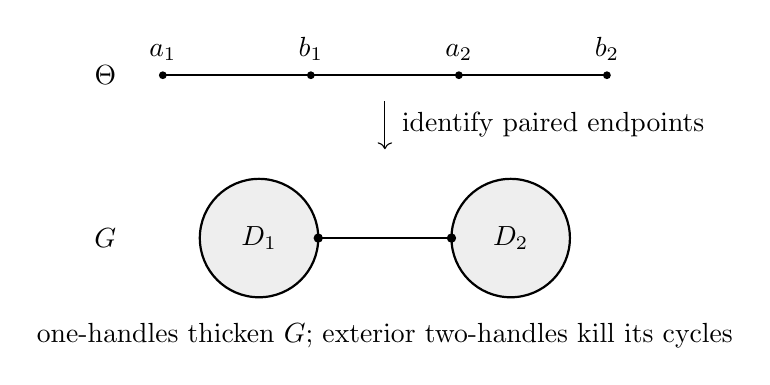
\begin{tikzpicture}[x=1cm,y=1cm,scale=.94]
 \draw[thick] (.4,2.2)--(6.4,2.2);
 \foreach \x/\s in {0.4/a_1,2.4/b_1,4.4/a_2,6.4/b_2}
   {\fill (\x,2.2) circle (1.5pt);\node[above] at (\x,2.27) {$\s$};}
 \node[left] at (-.1,2.2) {$\Theta$};
 \draw[->] (3.4,1.85)--(3.4,1.2);
 \node[right] at (3.5,1.53) {identify paired endpoints};
 \fill[gray!13] (1.7,0) circle (.8);
 \fill[gray!13] (5.1,0) circle (.8);
 \draw[thick] (1.7,0) circle (.8);
 \draw[thick] (5.1,0) circle (.8);
 \draw[thick] (2.5,0)--(4.3,0);
 \fill (2.5,0) circle (1.8pt);
 \fill (4.3,0) circle (1.8pt);
 \node at (1.7,0) {$D_1$};
 \node at (5.1,0) {$D_2$};
 \node[left] at (-.1,0) {$G$};
 \node[below,align=center] at (3.4,-1.02)
   {one-handles thicken $G$; exterior two-handles kill its cycles};
\end{tikzpicture}
\caption{The topology of the local domain, illustrated with two double
points.  The preimage tree thickens to an eight-disk.  The shaded disks
indicate the two-handle attachments only: their actual isotropic cores
attach to circles in $\partial P_1$ and lie off the immersed sheets.}
\label{top:domain-figure}
\end{figure}

\subsection{Removing positive double points and extending the grading}

\begin{lemma}\label{top:negative-doubles}
The immersion can be replaced on the disk $W$ by an oriented spin
Lagrangian immersion with only negative transverse double points.
It retains the boundary collar, its fundamental class, its integral
Maslov grading, and the homology-map properties in
Lemma~\ref{top:framed-source}.
\end{lemma}

\begin{proof}
Complete $P$ by its positive cylindrical end and extend the
immersed disk by its cylinder.  Remove the center of the
single-sheet radial ball supplied by Lemma~\ref{top:exact-domain}.
The punctured ball is a negative Liouville end.  The source
becomes an annulus $S^7\times\R$, with standard real-plane
Legendrian link $\phi_0\subset S^{15}$ at the negative end.
The punctured completion is simply connected, since removing
a point from a sixteen-manifold does not affect $\pi_1$.

We use the stabilization traces of
\cite[Lemma~3.2 and proof of Lemma~3.4]{eems}.  In source
dimension $2k$, a trace going outward from a Legendrian link
$\phi$ to its loose stabilization $\phi_1$ has one double
point of sign $(-1)^{k-1}$; the reverse trace has sign
$(-1)^k$.  For $k=4$ the signs are therefore
\begin{equation}\label{top:trace-signs}
 \phi\longrightarrow\phi_1:\ -1,
 \qquad \phi_1\longrightarrow\phi:\ +1.
\end{equation}
Put $m=-I(f_1)>0$.  Insert $m$ reverse traces in separated
radial collars near the puncture, ordered from the $m$-fold
stabilization $\phi_m$ at the innermost end to $\phi_0$
outward.  The negative link is now loose and the total signed
double count is $I(f_1)+m=0$.

Apply Eliashberg--Murphy's exact cancellation theorem
\cite[Theorem~2.3]{em-caps}.  Its hypotheses here are as
follows: the target is a simply connected Liouville manifold
with a negative end; the immersion is proper, self-transverse,
and has finitely many double points; its connected source has
dimension eight; the negative asymptote has one loose
component; and its signed double count is zero.  The
immersion is exact because $H^1(S^7\times\R;\R)=0$.
The additional width assumption of that theorem applies
only in source dimension three.  Its conclusion is a
compactly supported Hamiltonian regular homotopy to an
embedding.  Compact support preserves both cylindrical
tails, including the prescribed positive tail.

In the unchanged negative region, insert $m$ forward traces
from $\phi_0$ to $\phi_m$ and fill the center by the real
plane.  Equation~\eqref{top:trace-signs} shows that the filled
immersion has exactly $m$ double points, all negative.  Its
noncylindrical part is compact.  Apply a sufficiently long
negative Liouville flow in the filled positive completion to
bring this compact part inside $P$.  Backward flow exists
for all time; points inside $P$ cannot leave it backward,
and on the positive end it translates the cylindrical
coordinate.  The flow rescales the symplectic form, so
preserves Lagrangianity.  The positive cylinder remains the
same cylinder as a subset and crosses $\partial P$ in the
original collar.  Trim there and glue to the unmodified
immersion outside $W$.

The replaced source piece is a disk with collars.  A boundary
parameterization extends to a homeomorphism of disks, so the
old and new maps can be compared continuously relative to
the common complement.  As $T$ is aspherical, this disk
replacement preserves the homotopy class and the fundamental
class.  It also preserves the degree-two and degree-six
homology maps through the common complement.  Orient the
replacement compatibly.  Spin extends because the boundary
$S^7$ has a unique spin structure.  Finally every first
homology class is represented off the replaced disk; the
Maslov class therefore remains zero.  Choose the integral
grading with the original orientation parity.
\end{proof}

\begin{proof}[Proof of Proposition~\ref{top:brane}]
Apply local Lagrangian surgery at the negative double points
of Lemma~\ref{top:negative-doubles}.  We spell out the
grading choice, since it is the reason for using period four.
In symplectic coordinates the two sheets are
$\R^8$ and $i\R^8$.  The handle is
\[
 (s,x)\longmapsto\gamma(s)x,\qquad x\in S^7,
\]
where $\gamma$ rounds a corner from the positive real ray
to the positive imaginary ray through the first quadrant,
or to the negative imaginary ray through the fourth
quadrant.  The first ray is traversed inward and the second
outward.  With the usual monotone corner shapes these are
embedded Lagrangian handles: tangent vectors in the sphere
directions pair trivially, and their symplectic pairing
with $\gamma' x$ vanishes because $x\perp T_xS^7$.

These handles glue orientably exactly at a negative double
point.  For the coordinate orientations the two planes have
positive intersection sign in dimension eight, whereas
the handle gives opposite relative orientation marks at
its two ends.  Thus the negative intersection condition is
precisely the required orientation agreement.

Identify the ambient Maslov cover over each surgery ball
with the standard one.  For the phase lift $\arg\det/\pi$, a handle tangent frame
has determinant proportional to $\gamma'\gamma^7$.
Its total phase changes along the two corners are
\begin{equation}\label{top:surgery-phases}
 +3\quad\hbox{and}\quad-3,
\end{equation}
respectively; see also \cite[Lemma~2.4]{ekholm-smith}.
For example, along the first corner the initial argument
is $\pi$ and the final argument is $4\pi$.
The integral lifts of the two original sheet phases differ
by an odd integer, because their orientation marks are
opposite.  The two residues in \eqref{top:surgery-phases}
are the two odd residues modulo four.  Consequently one
of the two handles extends the grading modulo four at
each double point.  The choices are independent in
disjoint surgery balls.  The unique spin structures on
their boundary seven-spheres also give spin extensions.

Let $i_L:L\hookrightarrow T$ be the resulting embedded
Lagrangian.  Each oriented local surgery preserves its
pushed fundamental class.  Removing the pairs of
eight-disks and inserting $S^7\times[0,1]$ changes neither
$H_2$, $H_6$, nor $H^2$: the isomorphisms through the
common complement follow directly from the relative
homology sequence and Mayer--Vietoris.  They intertwine
the maps to $T$.  Thus all the properties of
Lemma~\ref{top:framed-source} asserted in the proposition
survive.  Finally \eqref{top:brane-cohomology}, extended
to $\C$, and de Rham's Theorem give exactness of the
restricted forms in $\Omega_{\C}$.
\end{proof}

\begin{corollary}[Ambient detection]\label{top:ambient-detection}
Let $r=2$ or $6$, and let $u$ be a closed complex $r$-form on $L$.
If
\[
 \int_L i_L^*\eta\wedge u=0
 \quad\text{for every closed complex $(8-r)$-form $\eta$ on $T$},
\]
then $u$ is exact.
\end{corollary}

\begin{proof}
The displayed pairings say that
$(i_L)_*([u]\cap[L])=0$ in $H_{8-r}(T;\C)$.
The relevant injection in \eqref{top:brane-injections}
and Poincar\'e duality give $[u]=0$.
\end{proof}

\section{Disk equations, compactness, and local gluing}
\label{local:section}

We now fix the symplectic form on $T$ once and for all.  The deformation
parameter will enter only through a relative closed two-form; it will not
change the equation for holomorphic curves.  This section constructs the
local analytic objects needed for the finite integrations in the next
section.  Particular care is needed at an unmarked boundary, at a transverse
boundary jump, and when several boundary nodes are smoothed simultaneously.

\subsection{Boundary labels and the relative weight}

Let $L\subset T$ be the embedded spin Lagrangian of
Proposition~\ref{top:brane}, with its
grading modulo four.  Set $J_*$ to be the flat complex structure determined
by $q+ip$.  We use a fixed sufficiently small uniformly tame neighborhood of
$J_*$ in the space of $\omega$-compatible almost complex structures.
All the structures below take values in this neighborhood.

There are countably many graph labels, arranged in layers indexed by
$\N\cup\{0\}$.  Each layer contains one copy of every scalar graph $G_k$,
$k\geq1$, and of $C$.  A label has the form
\begin{equation}\label{local:graph}
 X=\{p=A_Xq+\nabla f_X(q)\},\qquad
 A_X=h_0k\,1_8\quad\hbox{or}\quad S_-,
\end{equation}
where $f_X$ is a smooth periodic real function.  Layers are ordered
increasingly; within each layer the scalar slopes are ordered decreasingly,
followed by $C$.  Write $X\prec Y$ for this order, and $X^+$ for the copy of
the same slope in the next layer.  The order need not be a well-order; all
analytic constructions first use a finite sublist.  Each graph has the
orientation and spin structure from its base frame, trivial local system,
and the integral grading continued from the horizontal plane through
symmetric matrices.  In particular
\[
 \pi_2(T,X)=0,
\]
by the relative homotopy sequence and injectivity of $\pi_1(X)\to\pi_1(T)$.
Thus a graph supports no nonconstant holomorphic disk.

Choose the potentials so that all labels, including $L$, are pairwise
transverse and have no triple intersections.  In layer zero their Hessians
are as small as needed.  Require $f_{X^+}-f_X$ to be a sufficiently small
perfect Morse function; it may be chosen in the open set containing a small
split sum of cosines.  These choices are simultaneous: enumerate the
countably many required conditions, and use transversality of the
first-jet evaluation of a periodic function.  At each step the conditions
already imposed, as well as the perfect Morse condition, are open, and the
remaining transversality and avoidance conditions are residual in an
arbitrarily small open set.  Equivalently one may use the Baire theorem on
the product of these open sets of successive potential differences.

Our strip convention places the earlier boundary condition at height zero
and the later one at height one, with inputs at positive ends.  For graded
planes with positive rotation angles $\alpha_j\in(0,\pi)$, the degree is
\begin{equation}\label{local:degree}
 |x|=8+\vartheta_2-\vartheta_1-\sum_{j=1}^8\alpha_j/\pi.
\end{equation}
For two graph tangent planes this is the number of positive eigenvalues of
the second Hessian matrix minus the first.  To check this, keep their
difference fixed, move the first matrix to zero, and diagonalize the
difference.  Consequently the maximum of $f_{X^+}-f_X$ gives a unique
degree-zero generator
\[
 w_X\colon X\longrightarrow X^+,
\]
and all generators of $G_i\to G_j$, $i>j$, in layer zero have degree zero.
For arrows incident to $L$, degrees are taken modulo four.

Fix a complex symmetric matrix $M$ commuting with $D$, and put
$B=dq^tM\wedge dp$.  For $L$ and for scalar-slope labels choose forms
$\xi_A$ with $d\xi_A=i_A^*B$.  On $L$ these exist by the pullback-kernel
property proved above.  On a scalar graph we take
\begin{equation}\label{local:primitive}
 \xi_X=-(\nabla f_X)^tM\,dq.
\end{equation}
Indeed symmetry of $M$ makes the scalar linear part of $i_X^*B$ vanish,
and differentiation of \eqref{local:primitive} gives its remaining part.
For a polygon with fixed jump limits set
\begin{equation}\label{local:relative-weight}
 B_{\rm rel}(u)=\int u^*B-\sum_{\text{boundary arcs }a}
                         \int_a u^*\xi_{A(a)},\qquad
 \mathrm{wt}(u)=\qnov^{\int u^*\omega}\exp(tB_{\rm rel}(u)).
\end{equation}
Here $t$ is an ordinary formal variable and $\qnov$ is the Novikov monomial;
the coefficient field is specified in Section~\ref{cat:section}.
Only the unweighted specialization $t=0$ is used on words containing a
$C$-slope label.

\begin{lemma}\label{local:weight}
With the jump limits fixed, $B_{\rm rel}$ is invariant under homotopy
through maps with the prescribed boundary lifts.  It is additive on every
nodal splitting.  Thus the weight in \eqref{local:relative-weight} is
multiplicative on trees, coefficient by coefficient in $t$.
\end{lemma}
\begin{proof}
Apply Stokes to a homotopy cylinder.  Its boundary strips lie on the
prescribed labels, where $B=d\xi_A$, and cancel the variation of the arc
integrals.  The endpoint terms vanish because the jump limits are fixed.
On splitting a disk, integrals add over the components; the inserted
constant boundary paths at a node contribute zero.  This also proves the
assertion for refinements that retain relative classes at every vertex.
\end{proof}

\subsection{The area gap and the later-copy comparison}

\begin{lemma}[Uniform gap for a finite list]\label{local:gap}
For a finite transverse list of the labels and $L$, with no triples, there
is $\delta>0$ such that every nonconstant unforced disk or polygon with
these boundary conditions has area at least $\delta$.  The constant is
independent of the number of marked points and of the domain-dependent
compatible structure in the fixed neighborhood of $J_*$.  In particular
fix $\delta_L>0$ for nonconstant pure disks on $L$ with structure $J_*$.
\end{lemma}
\begin{proof}
Choose finitely many sufficiently small target charts.  A chart containing
a pair intersection meets precisely the two local exact sheets, with that
single intersection; elsewhere a sufficiently small chart meets at most
one sheet.  If the image has sufficiently small diameter, it lies in one
of slightly larger such charts.  In the two-sheet case every jump is at
the same point.  Normalize the two primitives to agree there.  Stokes
then gives zero area, even with repeated jumps; the one-sheet case is the
same.  Positivity implies that the map is constant.

Otherwise the connected image has a fixed positive diameter.  Remove
small disjoint neighborhoods of the finitely many pair intersections.
There is a regular image point outside them through which the image
crosses a ball of a fixed radius, meeting at most one local sheet.  Here
is the monotonicity estimate needed for this assertion.  Let $a(r)$ be
area in a subball and let $\ell(r)$ be the length, with multiplicities, of
its level contours.  Coarea and uniform compatibility give
$a'(r)\geq c\ell(r)$ for almost every $r$.  Each contour arc ending on the
local sheet can be closed there by a path whose length is at most a fixed
multiple of the arc length.  The primitive is exact on that sheet, so
this does not alter the Stokes computation.  A local primitive centered
at a point of each resulting loop gives the quadratic bound
$a(r)\leq C\ell(r)^2$.  Hence
\[
 a'(r)\geq cC^{-1/2}\sqrt{a(r)},\qquad a(r)\geq c_0r^2
\]
up to reducing the fixed radius.  All constants use target charts and
uniform compatibility only.  They do not use derivatives in the domain
of the almost complex structure.  This supplies the asserted gap.
\end{proof}

We impose a further smallness requirement on $X^+$.  It is the geometric
reason its eventual action on the new module will be invertible.

\begin{lemma}[Comparison with vertical fibers]\label{local:comparison}
For each $X$, its next copy $Y=X^+$ may be chosen with a number
$0<\epsilon_X<\delta_L$ and the following properties.  There are symplectic
coordinates in a tube about $X$ in which $X$ is horizontal, $Y$ is
$p=\nabla f(q)$ with $\operatorname{osc}f<\epsilon_X$, and each component
of $L$ in that tube meeting $X$ is a vertical patch at a point $q_j$.
Let $F_j$ be the full vertical fiber there.  Then:
\begin{enumerate}[label=(\roman*)]
\item Unforced $X,Y,L$ triangles of area at most $\epsilon_X$ coincide
literally with $X,Y,F_j$ triangles in the corresponding patch; no such
triangle joins different patches.
\item Every $X,Y,F_j$ triangle, with $X,Y$ corner $r$, has area
$f(r)-f(q_j)\leq\operatorname{osc}f$.  In particular the corner $w_X$
gives area $\Delta_j=f(\max)-f(q_j)<\epsilon_X$.
\item There are no nonconstant $X,L$ or $Y,L$ strips of area at most
$\epsilon_X$, and no nonconstant $X,F_j$ or $Y,F_j$ strips of any area.
\end{enumerate}
The same choices work for any of the allowed almost complex data after
pushing those data forward by the fixed symplectic coordinate change.
If $X\cap L=\varnothing$, choose $Y\cap L=\varnothing$ as well.
\end{lemma}
\begin{proof}
The integral shear $p\mapsto p-A_Xq$ and the gradient translation flatten
$X$.  Near a transverse intersection, the other sheet has equation
$q=q_j+\nabla_pg(p)$, with $dg(0)=0$.  A Hamiltonian shear, cut off in that
chart and generated using $g-g(0)$, makes it vertical while fixing the
horizontal sheet.  There are finitely many disjoint such charts.  By
compactness a sufficiently thin tube about the horizontal torus meets
$L$ only in these vertical patches.  A sufficiently close $Y$ remains an
exact graph throughout this transformation.

The crossing estimate of Lemma~\ref{local:gap}, applied away from the two
nearby graph boundaries, gives a fixed positive area cost for leaving
this tube.  It is uniform as $Y$ approaches $X$.  Choose $\epsilon_X$
below this cost and $\delta_L$, and then choose $Y$ with
$\operatorname{osc}f<\epsilon_X$.  A low-area curve stays in the tube and
its third boundary arc stays in one vertical patch.  Conversely, lift a
triangle with third boundary $F_j$ to the cover and use the primitive
$-p^tdq$.  The horizontal and vertical boundary actions vanish, while
the graph action is $-df$.  Stokes gives $f(r)-f(q_j)$.  Thus every such
triangle also stays in the tube and has the required correspondence.
A strip in a single patch has equal endpoint actions and area zero.
For the full vertical fiber the lifted graph and fiber have a unique
intersection, so this last argument applies without an area bound.
\end{proof}

\subsection{Harmonic domain data}

An $m$-disk has a distinguished boundary output followed
counterclockwise by its ordered inputs.  We use four sectors:
\begin{itemize}
\item pure $m_k$, with all boundary on $L$ and smooth input markings;
\item directed polygons with successive labels
$X_0\prec\cdots\prec X_k$, and all inputs and output transverse jumps;
\item mixed polygons with successive graph labels
$X_0\prec\cdots\prec X_b$, then $L$, with graph inputs followed by an
$X_b,L$ input and any number of smooth $L$ inputs;
\item pure $p_k$ disks with one interior output and $k$ cyclically
ordered smooth boundary inputs.  For nonconstant maps $k=0$ is allowed.
\end{itemize}
We count stable maps only.  The pure unary differential also has its
usual unstable term $d$ on differential forms.  Pure disks, including
all $p$ disks, use $J_*$.  In a sector with jumps, ignore all smooth and
auxiliary markings when choosing the equation.

For an ordered jump-arc list $\mathbf A=(A_0,\ldots,A_{m-1})$, let
$h_j(z)$ denote harmonic measure of its $j$th arc as seen from $z$.
Equivalently, send $z$ to the center of the disk and divide the arc's
angular length by $2\pi$.  Put
\begin{equation}\label{local:harmonic-J}
 J(z,x)=J_{\mathbf A}(h_0(z),\ldots,h_{m-1}(z);x),
 \qquad h(z)\in\Delta^{m-1}.
\end{equation}
The functions $J_{\mathbf A}$ are smooth on the closed simplices.

\begin{proposition}\label{local:data}
The functions in \eqref{local:harmonic-J} can be chosen simultaneously
with the following properties.
\begin{enumerate}[label=(\roman*)]
\item On a simplex face they agree with the function for the surviving
subsequence.  They equal $J_*$ near each vertex.
\item Near an edge joining labels $A,B$, they equal exactly
$J_{AB,h_B}$, for a height-dependent strip datum constant $J_*$ near
heights zero and one.  Take $J_{XL,\tau}=J_*$.
\item All nonconstant graph-pair strips and all directed polygons are
regular, including domain variations.  The comparison triangles of
Lemma~\ref{local:comparison}, with $L$ replaced by any $F_j$, are regular
for the pushforward of the same triangle data.
\end{enumerate}
No regularity of general mixed or pure maps is required.
\end{proposition}
\begin{proof}
First prescribe generic graph-pair data, supported in heights
$(0.1,0.9)$.  Ordinary strip transversality applies to these
$s$-independent data.  Its injective-point condition can be expressed as
injectivity of $(s,\tau)\mapsto(\tau,u(s,\tau))$: if an open immersed
patch had a same-height partner on every point, a Baire argument among
compact immersed patches would give overlapping branches
$u(s,\tau)=u(\phi(s,\tau),\tau)$.  The equation forces
$\phi(s,\tau)=s+c$; unique continuation would then contradict finite
energy for a nonconstant strip.  Critical images are negligible and
immersive points are dense.  Hence variations of $J_\tau$ near an
injective point kill any proposed cokernel element, also when the
variation is restricted to the indicated open height interval.

Extend by word size.  Require the pair formula where
$h_A+h_B>c_m$ and the vertex formula where $h_A>d_m$, using thresholds
increasing slightly with $m$, with $c_m$ close to one and $d_m$ close to
$0.94$.  Pair variations vanish near the endpoints, so these requirements
agree on overlaps.  In a local linear chart of compatible structures
near $J_*$, first extend the required collar formulas and then extend
the remaining boundary values over the simplex.  Inclusion--exclusion
in corner charts extends functions agreeing on intersecting faces;
a partition of unity combines the extensions.  A smooth retraction
into the chosen small neighborhood retains all already prescribed
values.

For $m\geq3$, a jump configuration together with one interior point,
modulo disk automorphisms, is identified with the open simplex by $h$:
after sending the point to the center, the successive arc lengths
recover all endpoints up to rotation.  There is a nonempty free open
set outside the prescribed edge and vertex collars.  Each fixed domain
has interior points mapping to this set under $h$: send any three of
its jumps to equally spaced circle points.  At the center every
individual weight is at most $1/3$ and every pair has total at most
$2/3$, so a neighborhood of the center is free.  There is an
immersive point there for a nonconstant solution.  A variation of
$J_{\mathbf A}$ supported near that simplex point isolates its domain
point, even if the map has multiple images.  The usual pairing with a
nonzero adjoint solution and unique continuation prove surjectivity
of the universal linearization.  A directed map is nonconstant because
there are no triples.  Sard--Smale therefore gives the required
regularity relative to all prescribed faces and collars.  Apply the
same argument also to the finitely or countably many auxiliary fiber
triangles using precisely the pushed-forward datum.  There are only
countably many words, classes, and such transversality requirements,
so the successive residual choices can all be made.
\end{proof}

\subsection{Boundary compactification and finite cuts}

\begin{lemma}[Only disk components occur]\label{local:disk-trees}
Every stable limit in the four sectors consists of disks joined at
boundary nodes.  Smooth nodes in a mixed sector split off pure $L$
disks.  At jump nodes the two ends have opposite transitions, and each
vertex has the corresponding subsequence of the original ordered
labels.  The same conclusion holds for positive-area $p_0$ disks;
there is no additional stratum in which the whole boundary collapses.
\end{lemma}
\begin{proof}
There are no nonconstant spheres because $\pi_2(T)=0$.  The disk vertices
in the doubled domain form a connected subtree: they are fixed vertices
of its real involution, and the path between fixed vertices is fixed.
Consequently other sphere trees could only hang from a disk at an
interior node.  A tree of $v$ constant spheres with one attachment and
at most one interior marking has at most $2v$ special points counted
with multiplicity, whereas stability requires at least $3v$; hence no
such tree occurs.

The issue when $p_0$ has no boundary markings is the possible collapse
of the entire real circle.  In the doubled dual tree the collapsed
boundary would be the midpoint of an edge whose branches are exchanged
by the involution.  This cannot coexist with a fixed disk vertex:
the path from a fixed vertex to that midpoint would be fixed, including
its final half-edge, contrary to exchanging the two half-edges.  Thus
all normalized components occur in conjugate sphere pairs.  In the
original half these are sphere components.  Positive area would force
one of them to be nonconstant, which is impossible.  This rules out
boundary collapse in the only sector where it is not excluded by a
boundary marking.

Following labels around a boundary smoothing proves the subsequence
assertion.  A smooth node on a graph would cut off a single-graph
subtree with no original inputs.  An outermost nonconstant component
would be a disk on that weakly exact graph, while a wholly constant
subtree is unstable.  Such a subtree is impossible.  Thus smooth
attachments in a mixed sector are pure $L$ branches.  On a limiting
core the omitted arcs have harmonic measure zero, so
Proposition~\ref{local:data}(i) gives exactly the equation of that vertex.
\end{proof}

We will verify compactness, including absence of neck drift, after giving
the explicit collar coefficients below.  Its finite-cut consequence can
already be stated.  For a finite list and a positive integer $N$ choose
\[
 0<a<\min(1,\delta_L,\delta),
\]
where $\delta$ is the gap of Lemma~\ref{local:gap}.  Define
\begin{equation}\label{local:cost}
 c_m(\beta,k)=\omega(\beta)+a(k-1),\qquad
 c_p(\beta,k)=\omega(\beta)+ak.
\end{equation}
Retain all stable types of cost at most $4N$, with their relative-class
refinements and all nodal types whether or not they are smoothable.

\begin{proposition}\label{local:finite}
This is a finite collection of compact moduli problems, closed under
normalized boundary and corners.  Costs add on every splitting, every
stable vertex has positive cost, and only finitely many relative classes
occur.  No discreteness of the symplectic period group is needed.
\end{proposition}
\begin{proof}
For an $m$ splitting with child arity $s$ and parent arity $k-s+1$,
$(s-1)+(k-s)=k-1$.  For a $p$ root the analogous equality is
$(s-1)+(k-s+1)=k$.  This proves additivity, including $s=0$.
A stable constant pure $m$ vertex has $k\geq2$, and a constant $p$
vertex has $k\geq1$.  A stable constant mixed vertex likewise has at
least three boundary special points; directed constants are excluded
by no triples.  Such vertices cost at least $a$.  Every nonconstant
$m$ vertex costs at least $\delta-a>0$, and every nonconstant $p$
vertex costs at least $\delta$.  Thus the cut bounds the number of
vertices, total area, and arity.  Only finitely many combinatorial
patterns and asymptotic generators occur.

For completeness the compactness argument, proved below in
Lemma~\ref{local:compactness}, is for the union over relative classes
with these bounds.  In a convergent sequence, maps on retained compact
cores are homotopic to their limits, and the remaining thin parts
have arbitrarily small diameter in the appropriate local one- or
two-sheet charts.  Contracting these parts and matching at the nodes
preserves the total relative class.  The class is therefore locally
constant in the compact stable-map space.  A finite subcover yields
finitely many classes.  The same reasoning retains any relative
refinement used to record the additive weight.  Positivity and
additivity show that every component of a boundary type stays in the
cut, proving boundary closure.
\end{proof}

\subsection{Real plumbing and quantitative collar coefficients}

Since all nodes are boundary nodes, we can use whole-disk projective
coordinates for every retained core.  Root a disk tree at its boundary
output, or at the disk carrying the interior output in the $p$ sector.
On a child use an upper-half-plane coordinate $z$ with its output at
infinity; on its parent put the attaching point at $a_e$.  The insertion
\begin{equation}\label{local:plumbing}
 \zeta=a_e+\rho_e z,\qquad \rho_e=e^{-\pi T_e},\qquad T_e\gg1,
\end{equation}
is real plumbing, using $-1/z$ as the child's nodal coordinate.  Cutting
out the corresponding half-disks and making this identification gives
another upper half-plane.  Iteration therefore identifies each core by
the restriction of a whole-disk biholomorphism.  This point will also
make the intrinsic normalizations in the next section compatible with
gluing.

Use node-specific projective coordinates varying smoothly in stabilized
component configurations.  They can be chosen equivariantly: a finite-order
orientation-preserving disk automorphism fixing a boundary point is the
identity, so a node stabilizer acts trivially on its incident disks.
Choose the germs on representatives of the node orbits and transport
them; invariant local slices for the finite stabilizer handle component
configurations.  Descendant arc endpoints in a parent coordinate have
the form $a_e+O(\rho_e)$, and exterior endpoints in a child coordinate
have reciprocals $O(\rho_e)$.  Iterated insertions give smooth expressions
in all plumbing parameters; apparent denominators stay separated by
using the nearest common ancestor coordinate.

\begin{lemma}[Harmonic collar estimates]\label{local:neck-coefficients}
On a jump neck $e$, write
\[
 \zeta-a_e=-e^{-\pi(s+i\tau)},\quad
 R\leq s\leq T_e-R,\quad 0\leq\tau\leq1,
 \qquad r_l=e^{-\pi s},\quad r_r=e^{-\pi(T_e-s)}.
\]
The transitions at the ends are an ordered pair $A,B$.  For sufficiently
large fixed $R$, the equation uses precisely its pair collar, and
\begin{equation}\label{local:angle-estimate}
 h_B=\tau+O(r_l+r_r),\qquad
 h_A=1-\tau+O(r_l+r_r),\qquad
 \sum_{C\ne A,B}h_C=O(r_l+r_r).
\end{equation}
On the parent half the difference from the partially broken parent
coefficient is $O(r_r)$; on the child half the corresponding difference
is $O(r_l)$.  These estimates hold after any prescribed finite number of
strip, target, and compact component-parameter derivatives.  Logarithmic
length derivatives have the same estimates, and a derivative with
respect to another length $T_f$ carries an additional factor
$O(e^{-\pi T_f})$, uniformly in the other large lengths.  In particular
all coefficients have uniformly bounded strip derivatives.

On a smooth matching neck the datum is exactly $J_*$ throughout a long
middle collar.  The same one-sided estimates hold at external jump ends.
\end{lemma}
\begin{proof}
Harmonic measure in the upper half-plane is the angle subtended by an
interval, divided by $\pi$.  For the two intervals adjacent to $a_e$,
the limiting angles in the displayed coordinate are $\pi\tau$ and
$\pi(1-\tau)$.  A displacement of a clustered endpoint is $O(\rho_e)$;
dividing by $|\zeta-a_e|=r_l$ gives $O(r_r)$.  A separated exterior
endpoint contributes an angle $O(r_l)$, with its reciprocal distance
bounded.  The smooth angle function and all of its derivatives on these
separated configurations give \eqref{local:angle-estimate} and the two
one-sided comparisons.  Differentiating $\rho_e$ logarithmically only
multiplies it by $-\pi$.  If an endpoint shift comes from a descendant
node $f$, its differentiated displacement is $O(\rho_e\rho_f)$ before
dividing by $r_l$; the same argument in an ancestor or nearest-common-ancestor chart treats all other cases.  This proves uniformity in every
other length as well as all finite derivative versions.

For large $R$ the total omitted weight is uniformly small, so the
simplex point lies in the pair neighborhood of
Proposition~\ref{local:data}; the coefficient is exactly $J_{AB,h_B}$.
At a smooth node only a pure $L$ branch is inserted.  No original jump
lies down that branch.  On the long collar the weight of $L$ is in the
vertex region, where the datum is exactly $J_*$.
\end{proof}

\subsection{Decay and compactness}

\begin{lemma}[Transverse ends and smooth-node decay]\label{local:decay}
At a jump limit $x\in A\cap B$, the operator
\[
 \mathcal A\xi=J_{AB,\tau}(x)\partial_\tau\xi,\qquad
 \xi(0)\in T_xA,\quad\xi(1)\in T_xB,
\]
on the interval is self-adjoint for the $\tau$-dependent compatible
$L^2$ metric, has compact resolvent, and has zero kernel.  In particular
it has a positive spectral gap.

On a sufficiently small-image long neck, solutions with no obstruction
support satisfy uniform exponential estimates from its two ends for
all positive derivatives.  At a jump the limiting value is the fixed
intersection; at a smooth node one separates a single movable value in
$L$.  On a strip $[0,T]\times[0,1]$, after removing fixed end collars,
one may take
\begin{equation}\label{local:two-sided-decay}
 |\nabla^jdu(s,\tau)|\leq C_j\bigl(e^{-\mu s}+e^{-\mu(T-s)}\bigr)
 \quad (j\leq j_0),
\end{equation}
for any preassigned finite $j_0$, with constants uniform near the given
nodal map.  The same estimates hold for small compact-core-forced
solutions, since their neck equations are unforced.
\end{lemma}
\begin{proof}
Put $g_\tau(v,w)=\omega(v,J_{AB,\tau}(x)w)$.  Compatibility gives
\[
 \int_0^1g_\tau(\mathcal A\xi,\eta)\,d\tau
   =\int_0^1\omega(\partial_\tau\xi,\eta)\,d\tau
   =-\int_0^1\omega(\xi,\partial_\tau\eta)\,d\tau
   =\int_0^1g_\tau(\xi,\mathcal A\eta)\,d\tau.
\]
The boundary term vanishes by Lagrangianity.  The adjoint has the same
boundary domain, which proves self-adjointness; the one-dimensional
elliptic estimate and compact embedding give compact resolvent.
Its kernel consists of constant paths in $T_xA\cap T_xB$, hence is zero.
Notice that no constancy of $J_{AB,\tau}$ in $\tau$ was used.

The full-cylinder inverse of $\partial_s+\mathcal A$ is obtained by
integrating the positive spectral subspace forward and the negative
subspace backward.  Its kernels are bounded by $Ce^{-\mu_0|s-s'|}$,
where $\mu_0$ is the spectral gap.  This gives the weighted estimate for
any logarithmic weight slope less than $\mu_0$; local elliptic estimates
give its Sobolev versions.  Straighten the two boundary sheets at $x$.
The nonlinear equation on a small-image neck differs from this model
by a small first-order term, a zero-order term bounded by $C|du|$, and
the controlled coefficients in Lemma~\ref{local:neck-coefficients}.
After a fixed shortening of the collar, absorb the small first-order
term in the cylinder estimate.  Cutting off at the two ends yields
\eqref{local:two-sided-decay}; differentiation and elliptic bootstrapping
give the asserted finite range of derivatives.

For a smooth node both boundaries lie on the same sheet.  Work first
in its cotangent tube, whose primitive vanishes on the zero section.
For a short path with endpoints on the sheet, its action is bounded
by a fixed constant times the square of its length: close it by a
short sheet path and use a centered primitive in a local chart.  If
$E(R)$ is the energy in $[R,T-R]\times[0,1]$, Stokes and this estimate
at the two slices give
\begin{equation}\label{local:neck-energy}
 E(R)\leq C\bigl(e(R)+e(T-R)\bigr)=-C E'(R),
\end{equation}
where $e(s)$ is slice energy, up to a fixed uniform comparison of
metrics.  Therefore $E(R)\leq C'e^{-R/C}$.  Small-energy regularity on
unit strips, with the uniform coefficient bounds above, gives
exponential decay of positive derivatives.  Integrating the first
derivative gives convergence to one value and the same two-sided
estimate measured relative to a middle boundary value.  This argument
also shows that the constant asymptotic mode must be retained, rather
than estimated by an invertible transverse model.  The argument for
two transverse sheets can alternatively use \eqref{local:neck-energy}
by closing each slice to their intersection along the sheets.
\end{proof}

\begin{lemma}\label{local:compactness}
For a finite list, fixed arity bound, and bounded area, the unforced
stable-map spaces of the four sectors are compact after adjoining the
disk trees of Lemma~\ref{local:disk-trees}.  There is no lost energy or
drift of the matching values.  On the cores the convergence is smooth,
and relative classes agree eventually with the total limiting class.
\end{lemma}
\begin{proof}
Apply the usual disk and strip rescaling procedure, retaining marked-point clustering scales as well as nonconstant bubbling scales.  The
required coefficient compactness holds here directly: harmonic
measures are bounded harmonic functions and have uniform derivatives
on interior hyperbolic balls.  Under any disk reparametrization,
clustered endpoints converge to a limiting configuration; on a
retained core their harmonic measures converge to the surviving ones.
Along a retained boundary arc the datum is constant in a vertex
neighborhood; on a jump collar use
Lemma~\ref{local:neck-coefficients}.  An interior blowup at scale much
smaller than the boundary distance sees constant-in-domain data.
Consequently any new gradient concentration gives an ordinary disk,
a transverse strip, or an interior sphere.  Spheres are impossible,
and each nonconstant level consumes the positive area gap.  There
are therefore only finitely many nonconstant levels, with precisely
the equations prescribed above.

After all these levels have been extracted, derivatives on the
remaining middle strips are small by small-energy regularity.  At
a jump, a short slice between two distinct compact sheets is close
to their finite intersection set.  Continuity makes it remain near
one intersection throughout each remaining thin strip.  For one
sheet, short slices already lie in its cotangent tube, even before
one knows that their longitudinal motion is small.  Thus
\eqref{local:neck-energy} applies in both cases.  The constants in the
single-sheet action estimate are uniform along the compact sheet;
it does not assume the image lies near a fixed point in advance.
Its exponential consequence and integration of $|du|$ show that the
central oscillation tends to zero.  This excludes slow travel along
$L$, as well as loss of energy, and identifies the two limiting values
at a smooth node.  Elliptic estimates give the claimed core
convergence.  Finally, thick-region homotopies and contractions of
these small thin parts within their prescribed local sheets identify
the total relative classes.  Stability and
Lemma~\ref{local:disk-trees} give the stated compactification.
\end{proof}

\subsection{Fixed-domain augmentation}

We specify precisely the local input from the established disk theory.
For a compact target, a compact relatively spin boundary Lagrangian,
and fixed tame $J$, compact-core obstruction data give finite-dimensional
disk charts and smooth evaluations; augmented boundary-evaluation
surjectivity gives an output submersion
\cite[Theorem~7.1, Condition~7.11, and Lemma~7.12]{fooo-i}.
The gluing theorem assumes surjectivity of the augmented component
operators and of the difference of their matching evaluations.
It gives local gluing and exponentially small positive length
derivatives on retained cores, also with domain parameters
\cite[Assumption~3.12, Theorems~3.13, 6.4, and 8.16--8.17]{fooo-decay}.
For a fixed datum our finite union of labels is an immersed Lagrangian
with transverse double points; retaining its boundary-lift sectors
provides the standard transverse-end Fredholm and determinant-line
setup \cite[Sections~4--5]{akaho-joyce}.  We next prove the extensions
needed for \eqref{local:harmonic-J} and for $p_0$.

At a component $u$ use high Sobolev order on its compact part.  At a
jump take weighted sections tending to zero at the fixed intersection.
At a smooth special point viewed as a cylindrical end, write a section
as its movable limit $a\in T_{u(z)}L$ plus a decaying section.  Small
positive weights are chosen below all nonzero indicial roots.  This
is the usual Fredholm formulation of a removable smooth boundary
point: the zero mode is the tangent limit, and homogeneous or
compact-core-forced solutions extend over the point.  Stabilize any
unstable nonconstant domain by interior marks constrained to transverse
target slices at immersive points, taking finite automorphism orbits.
One can do this also for an unbroken $p_0$ map.  The original interior
mark is retained, but no boundary mark is artificially made an output.

\begin{lemma}\label{local:augmentation}
For each component one can choose a finite-dimensional space $E$ and
an insertion $I:E\to C_c^\infty(\Lambda^{0,1}\otimes u^*TT)$ supported
in interior cores away from all markings, such that $D_u\bar\partial-I$
is surjective at fixed domain.  For every pure $m$ component the space
can be chosen so that
\begin{equation}\label{local:augmented-output}
 (\xi,e)\longmapsto
 (D_u\bar\partial\xi-Ie,\,\xi(z_0))
\end{equation}
is surjective as well.  Componentwise sums give a surjective nodal
operator with all smooth matching equations imposed.  The same holds
with a prescribed pure root-output variation.
\end{lemma}
\begin{proof}
The Fredholm cokernel is finite-dimensional.  At first Sobolev order
with target weighted $L^p$, $p>2$, smooth interior tests away from the
finite special points are dense, and hence span its quotient.  Choose
finitely many such tests.  To arrange \eqref{local:augmented-output},
apply the same argument to the operator restricted to sections with
$\xi(z_0)=0$.  Given any prescribed output value, first choose a
section attaining it and then solve its remaining equation with zero
output variation.  Bootstrapping transfers these conclusions to the
higher Sobolev orders.  Replace $E$ by the formal sum of its translates
under the finite stabilizer and average the auxiliary metrics.  This
makes the choice equivariant without reducing its image; injectivity
of the formal insertion is not needed.

At a smooth node the outgoing child is a pure $m$ component.  Starting
at the root, choose its solution with any required external output;
then solve each child with output value equal to the already chosen
parent value, and continue outward.  Formula
\eqref{local:augmented-output} permits this at each step.  Jump
matching is at a fixed transverse intersection and adds no tangent
matching variable.  This proves nodal surjectivity.  The pure constant
disk operator is already surjective with arbitrary constant boundary
value.  A constant mixed component has only an $X,L$ pair at the same
intersection, together with removable smooth marks, and has the
invertible transverse strip operator.  Thus constants require no
additional interior tests.
\end{proof}

\subsection{A uniform gluing estimate with several necks}

We give the uniform estimate explicitly, rather than invoking a fixed-$J$
gluing theorem for the domain-dependent equation.  Fix a stabilized nodal
map and the component augmentations of Lemma~\ref{local:augmentation}.
All constants below are uniform on a small relatively compact neighborhood
of its augmented nodal solutions.  The finitely many component operators
have a common indicial gap.  Choose a small positive weight $\delta$ below
one tenth of that gap and of the decay rates in
Lemmas~\ref{local:neck-coefficients} and \ref{local:decay}.

On an end use weight $e^{\delta s}$.  On a joined neck of length $T_e$
use a smooth version of
\begin{equation}\label{local:weight-function}
 w_e(s)=e^{\delta\min(s,T_e-s)}.
\end{equation}
The smoothing takes place in a fixed-width middle interval and changes
all norms by uniform factors.  At a jump, sections have zero asymptotic
constant.  At a smooth node write
\[
 \xi_e=a_e+\xi_e^{\rm dec},\qquad a_e\in T_{x_e}L,
\]
using fixed sheet-straightening coordinates; include $|a_e|$ separately
in the norm and weight only the remainder.  On a joined neck $a_e$ may
be the value at its middle boundary point.  On the finite set of cores
use the ordinary $W^{m,2}$ norms, and on remainders use
$\sum_{j\leq m}\|w_e\nabla^j\xi_e^{\rm dec}\|_{L^2}$.
Add the finite-dimensional domain and coefficient norms.  Denote the
resulting norm by $\|\cdot\|_{m,\delta,T}$, and use the corresponding
weighted $W^{m-1,2}$ target norm.  Here $m$ can be taken arbitrarily
large, but finite.

\begin{lemma}[Uniform augmented inverse]\label{local:inverse}
Fix any subset of nodes to remain broken.  For all other lengths
$T_e$ sufficiently large, the linearized thickened equation at the
preglued map is surjective, uniformly in every length.  After adding
finite-dimensional kernel coordinates measured on the cores and in
the coefficient variables, it has an inverse $Q_T$ satisfying
\begin{equation}\label{local:inverse-estimate}
 \|Q_T(\eta,b)\|_{m,\delta,T}
       \leq C_m\bigl(\|\eta\|_{m-1,\delta,T}+|b|\bigr).
\end{equation}
The same holds at sufficiently small thickened solutions, at fixed
domain, and with any prescribed pure root-output variation.
\end{lemma}
\begin{proof}
Choose core observables giving an isomorphism from the augmented nodal
kernel to a Euclidean space.  Together with the nodal operator and its
matching equations, these observables form a bounded isomorphism.
The same isomorphism works in the required finite range of Sobolev
orders and small weights: the indicial gaps do not change the index,
and elliptic regularity identifies its kernels.  Domain coordinates
can either be included or held fixed.  The output assertion uses the
augmented operator \eqref{local:augmented-output}.

Here is a bounded parametrix for the smoothed operator.  Split a target
section at each middle neck by a partition whose transition has fixed
width.  Transfer the two pieces to the corresponding semi-infinite
ends and extend them by zero.  Their one-sided weighted norms are
bounded by a fixed multiple of the joined norm, since on the support
of the left piece $s\leq T_e/2+O(1)$ and hence
\[
 e^{\delta s}/w_e(s)\leq e^{O(\delta)};
\]
the right side has the identical estimate.  Solve this forcing with
the nodal isomorphism, retaining all smooth matching equations and
the prescribed core coordinates.  The resulting two sections at a
smooth node have the same constant $a_e$.

On a component end cut off only the decaying part.  Take the left
cutoff equal to one through $T_e/2+2$, zero by $3T_e/4$, and with
$j$th derivative $O(T_e^{-j})$; take the reflected right cutoff.
The support of each split forcing lies where its own cutoff is one.
On the overlap set
\begin{equation}\label{local:splice}
 \xi_e=a_e+\beta_l\xi_l^{\rm dec}
                  +\beta_r\xi_r^{\rm dec}
\end{equation}
at a smooth node; at a jump omit $a_e$.  Thus the matching constant
is included once, not twice.  The joined weight is bounded by either
one-sided weight where that end is used, so the decaying terms have
uniform norm.  If the joined norm uses the actual middle value
instead of $a_e$, weighted Sobolev embedding gives
\[
 |\xi_e(T_e/2,0)-a_e|
       \leq C e^{-\delta T_e/2}
                (\|\xi_l^{\rm dec}\|_{m,\delta}
                 +\|\xi_r^{\rm dec}\|_{m,\delta}).
\]
Since $\|w_e\|_{L^2}\leq Ce^{\delta T_e/2}$, recentering by this
constant is still uniformly bounded.  This verifies the parametrix
bound including the zero modes.

Apply the smoothed operator to \eqref{local:splice}.  Commutators with
the cutoffs have norm $O(T_e^{-1})$.  The difference of the equation
coefficients from the corresponding component coefficients on a
cut end is exponentially small: its cutoff ends at $3T_e/4$, so the
opposite-end errors of Lemma~\ref{local:neck-coefficients} are at most
$Ce^{-\pi T_e/4}$ there, and pregluing errors have the analogous
map-decay bound.  At a smooth match, the limiting operator annihilates
a constant tangent vector.  Its zero-order coefficient on such a
vector is $O(|du|)$, so all errors involving $a_e$ have the same
exponential estimate after weighting; the choice of $\delta$ makes
this estimate summable.  Core-supported obstruction maps, constraints,
and kernel observables converge by their smooth core transport.
It follows that the parametrix $P_T$ satisfies
\begin{equation}\label{local:parametrix-error}
 \|\mathcal L_TP_T-\id\|
   \leq C_m\sum_{e\ \mathrm{smoothed}}
                      (T_e^{-1}+e^{-cT_e}),
\end{equation}
where $\mathcal L_T$ includes the kernel observables.  The number of
nodes is fixed.  Neumann inversion proves a uniformly bounded right
inverse.  The boundary-node Fredholm index formula subtracts
$\dim L$ for a movable smooth match and adds no matching dimension
at a nondegenerate transverse end.  It is exactly the nodal index
with the chosen smoothing lengths held fixed.  Hence adding the
same kernel observables gives index zero, so this right inverse is
an inverse.  All these estimates hold with any other nodes kept
broken.  Small changes of the map and coefficients preserve the
bound by a final Neumann inversion.
\end{proof}

\begin{figure}[ht]
\centering
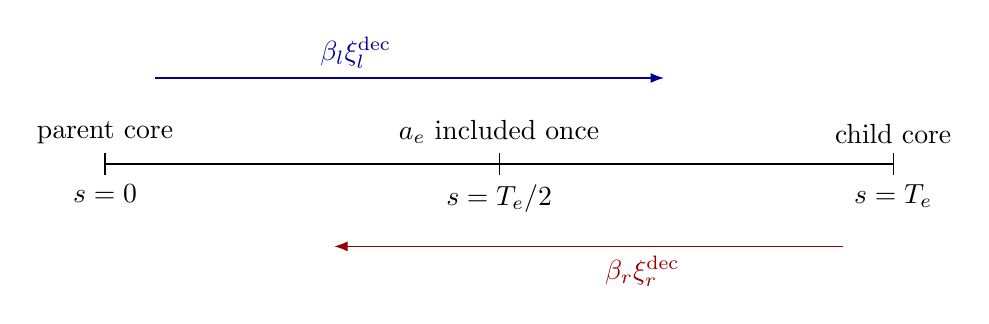
\begin{tikzpicture}[>=Latex,scale=.91]
 \draw[thick] (0,0)--(11,0);
 \draw (0,-.15)--(0,.15) (5.5,-.15)--(5.5,.15) (11,-.15)--(11,.15);
 \node[above] at (0,.15) {parent core};
 \node[above] at (11,.15) {child core};
 \node[above] at (5.5,.15) {$a_e$ included once};
 \node[below] at (0,-.15) {$s=0$};
 \node[below] at (5.5,-.15) {$s=T_e/2$};
 \node[below] at (11,-.15) {$s=T_e$};
 \draw[->,blue!60!black] (.7,1.2)--(7.8,1.2);
 \node[above,blue!60!black] at (3.5,1.2) {$\beta_l\xi_l^{\rm dec}$};
 \draw[<-,red!60!black] (3.2,-1.15)--(10.3,-1.15);
 \node[below,red!60!black] at (7.5,-1.15) {$\beta_r\xi_r^{\rm dec}$};
\end{tikzpicture}
\caption{A smooth matching neck.  The forcing is split in a fixed-width
middle interval.  The two decaying solutions are cut off over long
intervals, while their common tangent value is retained once.}
\label{local:neck-figure}
\end{figure}

The preceding proof also handles the controlled inhomogeneous collars
used later for ordinary continuation.  More precisely, suppose that,
after Hamiltonian transport of a limiting chord to an intersection,
the equation has an additional term $R_T(s,\tau,u)$ with bounded finite
strip derivatives, of size $O(r_l+r_r)$, and with differences from the
two partially broken equations $O(r_r)$ and $O(r_l)$ on the respective
halves.  Assume the differentiated versions in
Lemma~\ref{local:neck-coefficients} as well.  Each limiting end then
has a decaying forcing $O(e^{-\pi s})$.  The spectral inverse gives
decay at any smaller rate than the indicial gap and $\pi$; pregluing
has an exponentially small residual in a smaller weight, and the
same parametrix proof applies.  No nondecaying additive forcing is
permitted in this assertion.

\begin{proposition}[Local analytic chart contract]\label{local:charts}
For any prescribed finite integer $r$, choose sufficiently high Sobolev
order and sufficiently small positive weights.  Around each stable
map in the finite system of Proposition~\ref{local:finite}, the
component augmentations of Lemma~\ref{local:augmentation} give the
following local construction, also for $p_0$.

Allow finite-dimensional coefficient variables whose insertions are
supported on the normalized component cores, depend smoothly on
finitely many core jets and incidence markings, ignore the auxiliary
stabilizing marks, and have the core-transport and exponential
length-derivative properties of Lemma~\ref{local:neck-coefficients}.
At zero coefficients assume the fixed-domain augmentations above
are surjective.  Then the small pairs solving
\begin{equation}\label{local:thickened-equation}
 \bar\partial_Ju=I(u,\mathbf e)
\end{equation}
form local $C^r$ manifolds with corners modulo the finite map
stabilizers.  Corner coordinates are $q_e=1/T_e\geq0$, with $q_e=0$
meaning that node $e$ is retained.  Their normalized faces are exactly
the corresponding component solution spaces, matched over $L$ at
smooth nodes and over the fixed intersection at jumps.  Pure boundary
outputs are submersive on every stratum, also with the domain fixed.
Interior outputs need only be smooth.

These charts contain all sufficiently close solutions of
\eqref{local:thickened-equation}, including all partially broken ones.
Core observables, evaluation maps, and retrieval of transverse
stabilizing slices are $C^r$.  Changes between stabilizations retaining
the components and nodes at the comparison point are $C^r$ in these
coordinates.  Finally, outside sufficiently large fixed compact
interior cores, derivatives on hyperbolic unit vectors can be made
uniformly small on all these small-coefficient solutions.
\end{proposition}
\begin{proof}
We spell out both the nonlinear estimate and the length-derivative
estimate needed here.  Stabilizing slice equations are imposed with
marking positions free before division by disk automorphisms.  Their
transversality follows from the immersive incidence points, since
neither the equation nor the insertions uses those auxiliary marks.
Choose a finite collection $b$ of core kernel observables, including
coefficient and domain coordinates as necessary, which makes the
nodal linearization an isomorphism.  Near the nodal map they
parametrize its augmented solution stratum.  Preglue this nearby
nodal family with the prescribed $b$, cutting the decaying map parts
and retaining the matching values on $L$.

The residual of \eqref{local:thickened-equation}, including the
prescribed core observables, has norm at most
$C\sum_e e^{-cT_e}$ in a weight smaller than the component decay
rate.  On each core this follows from the smooth insertion transport
and Lemma~\ref{local:neck-coefficients}; in each middle neck it follows
from cutting exponentially decaying tails and the two one-sided
coefficient comparisons.  The same statement includes the controlled
additive errors described above, when present.

The nonlinear remainder satisfies, on a ball of fixed small radius,
\begin{equation}\label{local:quadratic}
 \|\mathcal N_T(\xi)-\mathcal N_T(\eta)\|_{m-1,\delta,T}
 \leq C\bigl(\|\xi\|_{m,\delta,T}+\|\eta\|_{m,\delta,T}\bigr)
                \|\xi-\eta\|_{m,\delta,T},
\end{equation}
with $C$ independent of the lengths.  Indeed ordinary Sobolev
multiplication on fixed-width cylinder charts has uniform constants;
$w_e\geq1$ puts the weight on the differentiated factor, while
Sobolev embedding bounds the undifferentiated one.  At a smooth
node use actual motions of the common point in $L$, not an affine
variation that violates the boundary condition.  In sheet-straightening
coordinates a constant such motion still solves the constant-map
equation.  Thus every nonlinear term on the neck involving the
constant has a derivative of a nonconstant part as a factor.  Its
weighted estimate is exactly the preceding product estimate, with
$|a_e|$ handled as a finite-dimensional variable.  The insertions
are on fixed cores, where ordinary high-order estimates apply.
Starting at a larger $m$ accommodates their finite jet dependence.

Apply the contraction theorem with the inverse in
Lemma~\ref{local:inverse} and the prescribed observables.  It gives a
unique small correction, with radius and estimates uniform in all
large lengths.  It works unchanged with an arbitrary subset of nodes
still broken, retaining their matching equations.  Conversely, a
nearby solution has the indicated stabilized domain by marked-domain
compactness.  Place its slice markings uniquely by incidence on the
retained cores.  Core closeness and Lemma~\ref{local:decay} put it in
the weighted implicit-function neighborhood: outside successively
larger cores the decaying tails are small in any strictly smaller
weight.  Hence the implicit construction captures every nearby
solution and has no extra local branch.  Lemma~\ref{local:augmentation}
and the version of the inverse with output prescribed prove
stratumwise output submersivity.  Kernel coordinates for this
statement may be chosen at fixed domain as in that lemma.

It remains to verify differentiability at simultaneous corners.
Identify domains under a change of $T_e$ by fixing vertex coordinates
on both sides and stretching only a middle part of neck $e$.
Trivialize compact component deformations while keeping their disjoint
nodal coordinate germs fixed.  Fix a finite range
\[
 m_0>m_1>\cdots>m_r>3,\qquad
 \delta_0>\delta_1>\cdots>\delta_r>0,
\]
with sufficiently large initial order.  The nodal and glued inverses
are bounded in this entire range.

We record the weight estimate used for a middle stretch.
Let $\chi_e$ be supported where
$\min(s,T_e-s)\geq\theta T_e$, for a fixed $0<\theta<1/2$, with
uniformly bounded strip derivatives up to the order in use.
For two successive weights $\delta'>\delta''$, using the weighted
target norm on the left,
\[
 \|\chi_e D_{\rm strip}\xi\|_{m-1,\delta'',T}
 \leq C e^{-\theta(\delta'-\delta'')T_e}
                   \|\xi\|_{m,\delta',T}.
\]
Indeed, the ratio of the two weights on this support is bounded by a
uniform multiple of
$e^{-\theta(\delta'-\delta'')T_e}$.  Here $D_{\rm strip}$ differentiates
components in the sheet-straightening coordinates: at a smooth match,
$D_{\rm strip}(a_e+\xi^{\rm dec})=D_{\rm strip}\xi^{\rm dec}$.
The estimate therefore applies to lower parameter variations as well
as to the map remainder.  A polynomial in $T_e$ multiplying the
left side is absorbed by reducing the exponential rate.
Differentiating the domain identification produces these middle
strip-derivative terms.  Its remaining zero-order terms involving a
movable constant contain a strip derivative of the map or a lower
variation, and obey the same weighted product estimate.
For a stretch on another neck $f$, the loss of weight there absorbs
its polynomial in $T_f$, uniformly in all the other lengths.

Differentiating the equation with
$b$ fixed uses the same inverse.  Explicit length derivatives of its
core coefficients and insertions are exponentially small.  On neck
$e$, stretching derivatives multiply a positive strip derivative of
the map, exponentially small near the middle in the next smaller
weight.  On any other neck, the differentiated harmonic coefficient
has the factor $e^{-\pi T_e}$ established in
Lemma~\ref{local:neck-coefficients}; it multiplies a strip derivative
of the map.  Constants occur only at smooth matches, where the
coefficient is $J_*$ and every relevant zero-order term has a factor
$du$.  These observations give, in the next norm of the finite range,
\[
 \|\partial_{T_e}u_T\|_{m_1,\delta_1,T}
           \leq C e^{-cT_e}.
\]
Here derivatives mean the covariant derivative under the just
specified core and middle-stretch identifications, including the
movable constants.

The same argument iterates.  At order $j$ the unknown highest
variation is acted on by the same augmented linearization; its
right-hand side is a sum of products of lower variations, differentiated
coefficients, and positive strip derivatives.  The uniform product
estimate, with a finite loss of Sobolev order, bounds every such term.
A middle-stretch derivative may contribute a polynomial in its length;
the difference between successive weights absorbs this polynomial
against the exponential tail.  If a mixed derivative contains
$\partial_{T_e}$, apply this induction with that derivative first.
Every subsequent tangential or length differentiation preserves an
exponential factor in $T_e$, in a weaker norm.  Thus for every
multi-index $\alpha$ with $1\leq|\alpha|\leq r$ and every $e$ in its
support, and for the allowed remaining parameter derivatives $D_b^\gamma$,
\begin{equation}\label{local:length-derivatives}
 \|D_b^\gamma\partial_T^\alpha u_T\|_{m_r,\delta_r,T}
              \leq C_{\alpha,\gamma}e^{-c_rT_e},
 \qquad |\alpha|+|\gamma|\leq r.
\end{equation}
Constants are uniform in the other large lengths and in which of
the other nodes are held broken.  This also bounds the restrictions
to every retained core and their movable limiting values.  Using
an index $e$ for which $T_e$ is largest among the differentiated
lengths absorbs every polynomial introduced by
$\partial_{q_e}=-T_e^2\partial_{T_e}$.

The limit as $T_e\to\infty$ is the corresponding partially broken
solution, by matching and implicit uniqueness.  Integrating the
exponential derivative bounds to that face, also after the allowed
tangential differentiations, proves $C^r$ extension in all $q_e$.
At a smooth node held broken, the estimate initially controls the
value and parameter variations uniformly on the punctured end.
In a smaller unpunctured neighborhood the equation has fixed $J_*$
and no obstruction support.  Removable-boundary-point regularity and
elliptic estimates, also for the differentiated equations, upgrade
these bounds to all needed evaluations at the node.  This completes
the differentiability proof for evaluations and core observables.

Two systems of auxiliary slices are recovered smoothly on retained
cores by their transverse incidence equations.  Compare them, if
necessary, through a third disjoint stabilization.  At the comparison
point all components are retained in each description; no chain of
nodes is contracted.  The real plumbing parameters for the same
node consequently satisfy
\[
 \rho'_e=v_e\rho_e,\qquad v_e>0,
\]
where $v_e$ is a smooth unit in the marked-domain coordinates.  After
retrieving the slices it is $C^r$ in the chart variables.  Therefore
\[
 T'_e=T_e-\pi^{-1}\log v_e,\qquad
 q'_e=\frac{q_e}{1-\pi^{-1}q_e\log v_e},
\]
which is $C^r$ also at $q_e=0$.  This argument concerns retained real
boundary nodes only.  The angular interior-node problem addressed
in the corrigendum \cite[Section~1]{fooo-corr} never arises here.
No compatibility with forgetting actual input markings is asserted
or needed.

Finally all insertions stay on compact interior cores.  Near ordinary
boundary arcs, the hyperbolic metric makes a bounded smooth derivative
small on its unit vectors as the boundary is approached.  In jump
ends and necks, hyperbolic unit vectors are bounded in strip
coordinates and \eqref{local:two-sided-decay} applies.  Choose the
cores large enough and then shrink the coefficient and implicit
neighborhoods.  These observations give the stated uniform smallness
off the cores, including for the nonzero-coefficient solutions used
in the next section.  Finite stabilizers act on this entire construction;
passing to their quotients gives the announced local charts.
\end{proof}

\section{Finite integration with exact boundary products}
\label{virt:section}

The local charts of the preceding section must be assembled so that Stokes'
theorem gives the \emph{same} integrations on every boundary factor.  We do
this at a fixed finite cut.  The coefficient variables of the obstruction
equations serve as continuous perturbation parameters; integrating their
normalized densities removes them.  Intrinsic incidence points on the
disks identify those variables on overlaps.  The point requiring care is
that a chart may carry more variables than its neighbor.  We arrange that
every such additional variable has identically zero insertion on the
overlap, so adding it is an ordinary product operation.

Throughout this section fix one of the finite boundary-closed systems of
Proposition~\ref{local:finite}, including its relative classes, and fix an
arbitrarily large finite differentiability order.  A \emph{map} includes
its domain, boundary lifts, and original markings, but excludes auxiliary
stabilizing markings and obstruction coefficients.  All map isomorphisms
preserve these original data.  In the $p$-sector we retain the actual
cyclically ordered input slots: cyclic reindexing is a symmetry between
these labeled spaces, not an additional quotient.

\begin{theorem}[Finite integration package]\label{virt:finite-integration}
For this finite system there are oriented integration correspondences for
the stable pure $m$, directed, mixed, and interior-output $p$ sectors,
including $p_0$, with the following properties.
\begin{enumerate}[label=\textup{(\roman*)}]
\item Pullbacks of evaluation forms can be integrated in the virtual
dimension.  The pure boundary-output correspondences give differential
forms by submersive pushforward.  The interior output of a $p$-operation
may be tested against any smooth ambient form; no submersivity of that
evaluation is required.
\item Stokes' theorem holds exactly with the normalized boundary.  On a
face with distinguished nodes its integration is the product of the
component prescriptions, using an evaluation fiber product over $L$ at
a smooth node and a product over the fixed intersection generator at a
jump node.  These identifications agree on iterated corners.
\item The prescriptions are equivariant under cyclic reindexing of $p$
inputs, with the determinant and form-permutation signs.  Only actual
finite map isotropy contributes an orbifold integration factor.
\item A regular zero-dimensional type with empty boundary and trivial
isotropy has its ordinary signed count.  In particular this applies to
the rigid directed spaces and to the low-area rigid comparison triangles
of the preceding section.  The constant $p_{1,0}$ correspondence is
ordinary integration on $L$, with a fixed orientation sign.
\end{enumerate}
All assertions hold coefficientwise after multiplying each relative-class
term by its energy monomial and, when defined, by
$\exp(tB_{\rm rel})$.  The choices need only be made at the specified
finite cut.  Operation signs and the unstable de Rham differential are
specified in the next section.
\end{theorem}

We prove the theorem by constructing and comparing the integrations.
The framework for disk obstruction charts in
\cite[Theorem~7.1 and Condition~7.11]{fooo-i} and the componentwise
framework of \cite[Theorems~2.5, 5.3--5.4 and Remark~6.1]{fooo-ii}
motivate the construction.  The intrinsic probes, the $p_0$ treatment,
and the precise overlap integrations below are part of our argument.

\subsection{Intrinsic incidence probes}

Write $\mathbb D$ for the open unit disk, equipped with its hyperbolic
metric.  A \emph{probe} consists of the following finite data:
\begin{enumerate}[label=\textup{(\alph*)}]
\item two ordered codimension-two target slices $S_1,S_2$, with compact
subpatches $K_i\subset\operatorname{int}(S_i)$;
\item a positive lower threshold for the least singular value of the
normal incidence derivative at each point, computed using the hyperbolic
metric on the disk, and bounds
$0<d_-\le d_+<\infty$ for the distance between the two points;
\item an oriented, even-dimensional real vector space $E$ and a linear
map from $E$ to smooth $TT$-valued real one-forms compactly supported in
$\mathbb D$, using the fixed parallelization of $TT$.  The map has at
least one dummy coordinate with zero image.
\end{enumerate}
Choose a compact set $K\Subset\mathbb D$ containing all these supports,
the origin, and every possible normalized second point at distance in
$[d_-,d_+]$ from the origin.  Choose
$0<\epsilon<\operatorname{dist}(K,\partial\mathbb D)$.

An occurrence on an actual map $\mathbf u$ is an ordered pair of distinct
interior points $(w_1,w_2)$ of one normalized disk component such that
$u(w_i)\in K_i$ and all the closed thresholds hold.  There is a unique
disk biholomorphism
\[
 \varphi:\mathbb D\longrightarrow D_v,
 \qquad \varphi(0)=w_1,\qquad
 \varphi(r)=w_2\quad\text{for some }r\in(0,1).
\]
If the original interior output mark belongs to this component, require
its $\varphi$-coordinate to be at distance at least $\epsilon$ from $K$.
There is no restriction involving the order or position of the boundary
special points.  We use every occurrence on the representative map,
without quotienting the occurrence set by automorphisms.

The probe also carries a smooth scalar cutoff $0\le\chi\le1$ along
transverse incidence branches.  Its support lies within strictly stronger
versions of the closed conditions just imposed.  For instance, choose
bumps on the full slices supported inside $K_i$, a distance bump supported
inside $(d_-,d_+)$, and smooth functions of the normal derivative matrices
supported where the least singular values exceed the selected
thresholds.  Such derivative cutoffs exist on the finite-dimensional
space of matrices; they can be made invariant under orthogonal changes
of frames.  For the interior mark use a smooth function on the normalized
disk, zero on a neighborhood of $K$ and equal to one near the circle,
with support inside the avoidance condition.  This factor is defined to
be one if the component has no original interior mark.  Given a desired
transverse pair with strict margins, these choices can be made with
$\chi=1$ near that pair.

\begin{lemma}[Finiteness and continuation of probes]\label{virt:probes}
For a finite list of probes, every actual stable map has finitely many
occurrences.  If actual maps converge stably, each sequence of occurrences
has a subsequence converging, in a whole-disk normalization, to an
occurrence on one disk of the limiting map.  Each limiting occurrence
continues uniquely to nearby maps, including sufficiently close ambient
maps in stabilized plumbing neighborhoods.  The continuations are
equivariant under map isomorphisms.
\end{lemma}

\begin{proof}
There is a positive lower bound for the area in a hyperbolic radius-one
ball about the first incidence point.  Otherwise recenter a sequence of
such balls by disk isometries.  The harmonic-measure coefficients have
uniform bounds of every required order on compact interior balls; only
finitely many equation data occur at this cut.  Interior small-energy
regularity would force the derivative at the center to tend to zero,
contrary to the positive lower incidence threshold.  This argument is
applied here to actual, unforced maps.

In a stably convergent sequence, the energy identity allows compact
interior cores of the nonconstant limiting disks to carry all but less
than this lower bound of the sequence's energy.  A radius-one ball at an
occurrence must therefore meet one of these cores.  The component
reparametrizations are restrictions of whole-disk biholomorphisms, as in
the boundary plumbing construction.  In the normalization of the core
that it meets, the first point belongs to a fixed compact interior set;
the upper bound $d_+$ puts the second in another such set.  After passing
to a subsequence both converge there.  Smooth core convergence preserves
the closed slice, derivative, and distance conditions.  If the limiting
component carries the original interior mark, its coordinate converges
too, preserving mark avoidance.  We obtain an occurrence on a single
limiting disk.

The derivative of the incidence equation with respect to the position
$w_i$ is an isomorphism onto the two-dimensional normal space of $S_i$.
The implicit function theorem, using the full slice rather than its
compact subpatch, therefore continues the point uniquely under
sufficiently small $C^2$ core perturbations and domain deformations.
The same argument applies simultaneously to the ordered pair.  For a
fixed map, an infinite occurrence set would have an accumulation point
by the preceding compactness argument, contradicting this local
uniqueness.  Thus the set is finite.  A sequence of occurrences on nearby
actual maps that was not among the continued branches would likewise
contradict compactness and uniqueness.  Distinct continued branches
remain distinct after shrinking.

Finally, all conditions and the normalization are invariant under disk
biholomorphisms.  Changing the core identifications continues the same
incidence branches; central finite automorphisms merely permute them.
This proves the equivariance assertion.
\end{proof}

For a chart centered at $\mathbf u$, let $O_{\mathbf u}$ be the occurrences
at its center, and continue this fixed finite set over the chart
neighborhood.  \emph{Do not retest the closed conditions} at a nearby
map $\mathbf x$.  Set
\[
 E_{\mathbf u}=\bigoplus_{o\in O_{\mathbf u}}E_o.
\]
Transport the one-forms for $E_o$ by its actual normalization
$\varphi_o(\mathbf x)$ and project to $(0,1)$-type for the equation on
$\mathbf x$.  Denote the resulting insertion by $I_o(\mathbf x)$.
The coefficient space is a formal direct sum: the insertion maps need
not be injective or have independent images.

These insertions satisfy the smooth core-transport hypotheses of
Proposition~\ref{local:charts}.  Incidence positions are recovered smoothly on
the cores.  Whole-disk normalizations commute with the projective
insertions in real boundary plumbing, and their expressions on retained
cores have no singular scaling.  Projection to the varying $(0,1)$-type
has the length-derivative estimates established there.  The derivative
and mark cutoffs are smooth finite-order core observables.  If the
original interior mark enters the disk from a different component under
smoothing, its coordinate tends to the unit circle, so its avoidance
factor is identically one near the broken configuration.  Thus on every
normalized face both the insertions and their cutoff factors restrict
\emph{exactly} to the component rules.

\subsection{A finite family of regular thickenings}

At each actual map choose two distinct immersive interior points on each
nonconstant disk, transverse slices through their images, and a probe
with strict margins at this pair.  Its compactly supported test forms
can be chosen to span the finite-dimensional cokernel of the fixed-domain
operator.  On a pure $m$ component choose them to span the cokernel of
the operator augmented by its boundary output evaluation.  Compact
interior tests away from the original interior mark suffice by
Proposition~\ref{local:charts}.  Enlarge the coefficient space to even dimension
and include a dummy zero direction.  Include a probe also on a regular
nonconstant component, since it will be useful for isotropy.

Constant components require no such tests.  A pure constant component
has the regular real-disk operator with freely varying value in $L$.
A constant mixed component has only an $X,L$ pair, two opposite jumps
at one intersection, and possibly removable smooth $L$-marks.  Its
map operator is the invertible transverse strip operator.  A stable
constant directed component cannot occur: three distinct boundary labels
have no common point, whereas a two-ended constant strip is unstable.

The chosen active branches persist on nearby actual maps.  In particular,
when several components join, the inverse construction of
Proposition~\ref{local:charts} uses their continuing probe blocks.  All smooth
matching equations are solved using pure child output submersivity;
one may still prescribe the pure parent output.  This proves the
required fixed-domain augmentations for each joined component.  A nearby
nonconstant joined component contains a continuing probe: a cluster of
constant components cannot become a nonconstant actual component with
energy tending to zero, by the area gap.  Compactness now gives a finite
cover of all actual moduli at the cut by such neighborhoods.  Take the
union of their probe lists and allow every probe on every disk.
Additional coefficient directions preserve the augmentations.

For small coefficients we use the space of pairs satisfying
\begin{equation}\label{virt:thickening}
 \bar\partial_J\mathbf x
   =\sum_{o\in O_{\mathbf u}}
        \chi_o(\mathbf x)I_o(\mathbf x)e_o,
 \qquad e_o\in E_o.
\end{equation}
After auxiliary stabilization and quotient by actual map isomorphisms,
Proposition~\ref{local:charts} gives a regular orbifold with corners near
$(\mathbf u,0)$.  Its dimension is the virtual dimension plus
$\dim E_{\mathbf u}$.  Pure boundary output is submersive on every
stratum.  Auxiliary incidence marks can be chosen in automorphism orbits
away from the compact obstruction supports: nonconstant maps have
immersive points in any remaining interior collar, by unique
continuation.  The auxiliary mark variables and slice constraints cancel
in the tangent determinant.  Orient the thickening by the virtual
Fredholm and marked-domain determinant, followed by the oriented
coefficient directions.

Here is the isotropy check, including the sector without boundary inputs.
For $p$, root the disk tree at its interior mark.  If a nonconstant root
has a nonidentity finite stabilizer, an ordered pair of distinct interior
anchors cannot be fixed: a disk automorphism fixing both is the identity.
The stabilizer consequently permutes probe occurrences nontrivially.
Their dummy coefficients, which are tangent kernel directions at zero,
detect this permutation even after quotient by infinitesimal
reparametrizations.  A constant root has at least one boundary special
point by stability; with only one, its stabilizer is trivial.  A
nontrivial rotation about the interior mark must permute at least two
boundary special points nontrivially and acts effectively on their
angular configurations modulo simultaneous rotation.  Indeed the tangent
space of these configurations is $\R^r/\R(1,\ldots,1)$ for $r\ge2$;
no nonidentity permutation induced by a finite rotation acts trivially
on it.  Fixed-domain augmented surjectivity allows all these domain
variations in the thickening.  An automorphism identical on the root is
identical down the tree, because a finite disk automorphism fixing a
boundary parent point is the identity.  The same last argument makes
boundary-rooted $m$ stabilizers trivial.  Thus the charts can be taken
effective.  For an unbroken nonconstant $p_0$ map the two interior anchors
provide exactly the stabilization and effective action just described.

\subsection{Comparison of charts without changing the equation}

\begin{lemma}[Joint charts and inactive coefficients]\label{virt:joint-charts}
The thickening neighborhoods can be shrunk with the following properties.
Every incidence branch with potentially nonzero cutoff is tracked there.
On an overlap, branches common to two charts have identical coefficient
coordinates and insertions.  Every branch belonging to only one list has
identically zero cutoff near the overlap.  After adding these inactive
blocks to the other list, the two equations define the same local space
of pairs, with the same evaluations, isotropy, and determinant orientation.
The comparison is smooth to the prescribed finite order, including on
faces with any specified nodes retained.
\end{lemma}

\begin{proof}
First exclude untracked active branches for ambient maps, not merely
actual ones.  Choose fixed compact cores and sufficiently small gluing
neighborhoods.  Outside the cores the derivative on hyperbolic unit
vectors can be required to be smaller than every probe's lower
threshold.  At ordinary boundary arcs this follows from smooth boundary
control and the blowup of the hyperbolic metric; at long necks and jump
ends it follows from the decay estimates in Lemma~\ref{local:decay},
where hyperbolic unit vectors have bounded strip-coordinate norm.
These restrictions are valid also for the small-coefficient solutions,
whose obstruction terms remain on the specified cores.  Consequently
any pair in the inner cutoff supports must lie on the continued compact
cores.  Core closeness and the implicit uniqueness in
Lemma~\ref{virt:probes} identify it with a tracked branch.  The strict
margin between the cutoff support and the closed occurrence conditions
is essential: a branch failing the latter at the center stays outside
the former on a neighborhood.

We next make precise that the underlying-map comparisons used here have
no extra multiplicity.  The core convergence in these neighborhoods,
together with arbitrarily small oscillation in the omitted necks and
ends, has unique stable-map limits up to isomorphism.  To prove this,
suppose a sequence admits two such limits.  Stabilize using the markings
for both limits and pass to a common stable marked-domain limit.  Extra
comparison marks may be displaced slightly to avoid coincidences.
Forgetting one or the other marking system recovers the two given domain
limits.  A component contracted in one description has constant limiting
map, by core convergence or the small oscillation on its omitted region.
The maps on every retained component agree in the common refinement.
After forgetting all auxiliary marks and contracting unstable constant
components, both limits therefore give the same stable map.  This uses
no holomorphic equation on the retained cores.

It follows in particular that, after shrinking about a center, lifts of
the same map to its slice gauge differ only by its central finite
automorphisms.  Otherwise compare a sequence of conflicting gauge lifts
by the preceding marked convergence.  Their limiting identifications
are central automorphisms, which preserve the chosen slice systems with
their induced relabelings.  Transverse incidence then makes the continued
marks exactly identical up to that relabeling, a contradiction.  This
also shows that underlying isomorphisms lift to the gauges.  Stability is
preserved nearby, either by the original domain specials or by the
persistent immersive cores of nonconstant components.

On an overlap take the union of the two continued branch lists, identifying
coinciding branches by transverse uniqueness.  A branch missing from
one list is outside its inner cutoff support throughout a smaller
comparison neighborhood by the first paragraph; hence its contribution
to Equation~\eqref{virt:thickening} is identically zero there.  Adding its
coefficient block thus takes a product with $E_o$, rather than changing
the equation.  Redundancy among the active insertions does not affect
this assertion: coefficients remain part of the pair and are never
quotiented by the kernel of their insertion.

For smoothness recover both sets of stabilizing marks by their transverse
incidences, or compare through a third marking system disjoint from them
at the point in question.  Each stabilization retains every component
of that point.  Adding and forgetting comparison marks therefore
contracts no component there.  Every retained node represents the same
single domain divisor on the two sides, so its real plumbing parameters
differ by a smooth positive unit.  The inverse-length changes are smooth
by Proposition~\ref{local:charts}; there is no multiplication of plumbing
parameters along a contracted chain.  This argument also applies on a
normalized face, keeping its distinguished nodes.  Core observables,
slice positions, and kernel coordinates compare smoothly, and the
weighted neighborhood conditions are preserved after shrinking by the
same decay estimates.  It applies with small nonzero coefficients,
since the padded equations are literally identical.

These comparisons retain the map isomorphisms, acting on the branch
variables as well.  The auxiliary mark and constraint determinants
cancel, and adjoining a block appends its oriented determinant.
Permuting entire blocks preserves orientation because their ranks are
even.  This proves all the claims.
\end{proof}

\subsection{Buffered partitions depending only on maps}

Choose for each probe a smooth compactly supported top-form density
$\Xi^\hbar$ on its oriented coefficient space, of integral one and
supported in $|e|<\hbar$.  The same density is used at every occurrence
of that probe.  In a chart let
\begin{equation}\label{virt:density}
 \Xi_{\mathbf u}^\hbar
       =\bigwedge_{o\in O_{\mathbf u}}\Xi_o^\hbar(e_o).
\end{equation}
It is closed, and its definition is unaffected by permutation of the
even-dimensional blocks.  Inactive blocks still carry their full
densities.

We must localize on maps without selecting only some coefficient
representatives of a map.  The following elementary consequence of the
chart construction supplies this point.

\begin{lemma}[Buffered partitions]\label{virt:buffered-partitions}
There are finitely many trimmed thickening charts $V_\alpha$, nonnegative
map functions $f_\alpha$, and a common sufficiently small $\hbar>0$,
such that near all density supports:
\begin{enumerate}[label=\textup{(\roman*)}]
\item the zero extensions of the $f_\alpha$ pull back smoothly to every
chart, and $\sum_\alpha f_\alpha>0$;
\item each $f_\alpha$ has support, with a buffer, strictly inside its
chart, relative to the actual nodal corners;
\item if a map is in that support, the chart represents every assignment
at the common small support scale that solves its equation for that map.
This includes every free choice of coefficients in any blocks made
inactive during an overlap comparison.
\end{enumerate}
Thus $\lambda_\alpha=f_\alpha/\sum_\beta f_\beta$ is a partition on
the map projections of the relevant pairs.  It is independent of which
small coefficient assignment represents the map.
\end{lemma}

\begin{proof}
Around each center choose nested coordinate neighborhoods with compact
closures inside a larger thickening chart, and trim inside the larger
one.  Here compactness refers to the finite-dimensional chart, with its
actual corner faces retained.  Its local coordinates can be chosen from
the coefficient coordinates and finitely many smooth functionals of the
map on retained cores, together with stabilized domain variables and
inverse neck lengths.  Indeed these functionals separate the augmented
kernel: after fixing the coefficients, a homogeneous kernel section
vanishing on open cores vanishes by elliptic uniqueness.  Finitely many
tests suffice on this finite-dimensional kernel, and the inverse
function theorem supplies local coordinates.

Consequently bounds on finitely many map and domain observables keep a
solution in a smaller coordinate neighborhood uniformly for all
sufficiently small coefficients.  Take a smooth bump of these
observables, positive at the center and supported with a strict interior
buffer.  Average over the central finite group.  The observables use
continued slice gauges, whose only ambiguity is that group by
Lemma~\ref{virt:joint-charts}; the averaged function is therefore a
function of the map.  These bumps do not depend on its coefficients.
Select finitely many so that their positive neighborhoods cover the
actual compact locus, and include their cyclic translates in the
$p$-sector.

We justify the required uniformity before fixing the support radius.
Consider a sequence of pairs in the trimmed closures whose coefficients
tend to zero.  There is a subsequence converging in a larger chart to
$(\mathbf v,0)$, where $\mathbf v$ is actual.  Every applicable open
gauge neighborhood of $\mathbf v$ then contains the maps in that
sequence.  Transfer their common branch coefficients to such a gauge
and choose arbitrary coefficients tending to zero in its inactive
blocks.  The local chart parametrizes all small solutions of its
equation, so every resulting pair tends to $(\mathbf v,0)$ in that chart.
Uniqueness of the map limit and slice positions excludes any other
nearby lift.  Some $f_\alpha$ is positive at $\mathbf v$; thus failure
of positivity at every sufficiently small coefficient scale would
contradict this subsequence argument.

The same argument proves the all-assignments assertion.  If it failed
at arbitrarily small scales, take an offending map in a projected cutoff
support and an alternative assignment at that scale solving the same
equation.  A lift of the map in the originating cutoff support lies in
its compact buffered region.  Pass to its actual limit.  The alternative
assignment tends to zero; after branch transfer and arbitrary padding
it must lie near $(\mathbf v,0)$ in the originating chart, by its local
completeness.  The strict buffer contradicts its asserted exclusion.
This reasoning includes the inactive variables and any kernel among
the active insertions.  Finiteness of the chart collection permits one
uniform scale.  One may first obtain these conclusions for coefficients
bounded by $2\hbar$, and then put the densities inside the $\hbar$ balls.

Finally consider smoothness of the zero extensions at this fixed small
scale.  Near a projected cutoff support, the compact buffer and
uniqueness of underlying-map limits put every comparison in the same
open slice gauge.  The map observables there compare smoothly by
Lemma~\ref{virt:joint-charts}, and the all-assignments property permits
every small coefficient transfer needed for that comparison.  Away
from the projected support the cutoff is identically zero on a
neighborhood of the density support.  Its extension is therefore
smooth in either case.  The same buffer applies to its derivatives.
Normalizing the sum now gives the asserted partition.
\end{proof}

This construction uses no global parameter space of constant rank.
Only the local pairs and the map functions in
Lemma~\ref{virt:buffered-partitions} enter the integration.

\subsection{Patching, Stokes, and boundary composition}

For a product $\alpha$ of pulled-back evaluation forms, in its specified
order, define
\begin{equation}\label{virt:integral}
 \mathcal I_{\mathcal M}(\alpha)
   =\sum_\gamma\int_{V_\gamma}
           \lambda_\gamma\,\alpha\wedge\Xi_\gamma^\hbar.
\end{equation}
Integrals are ordinary orbifold integrals: in a local finite quotient
they are divided by its actual group order.  The density is put last.
The integral vanishes unless the remaining form degree is the virtual
dimension.  Compact support in the coefficient directions and the
buffered map support make every integral compactly supported away from
the artificial trimming boundary.  At a pure boundary output the same
formula, using submersive fiber integration, gives a differential form.
We characterize its order convention by placing the output test form
first.  Submersivity on every stratum ensures that its boundary
pushforwards are defined by the same rule.

\begin{lemma}[Exact patching and Stokes]\label{virt:patching}
Equation~\eqref{virt:integral} is independent of the buffered partition
and of the slice gauges used to compute it, for the chosen probes and
densities.  It is unchanged by adjoining inactive blocks.  It satisfies
\[
 \mathcal I_{\mathcal M}(d\alpha)
       =\mathcal I_{\partial^{\rm norm}\mathcal M}(\alpha),
\]
where the right side has the induced boundary orientation.  Its
prescription on a normalized face is exactly the product prescription
from its component moduli, with the corresponding matching conditions.
\end{lemma}

\begin{proof}
On a buffered overlap identify common branch coordinates and take the
union $O$ of the branch lists.  By Lemma~\ref{virt:joint-charts} its pair
space is locally the first chart times the missing inactive blocks, and
also the second chart times its missing inactive blocks.  Over every
map in the cutoff support these products contain the full coefficient
supports by Lemma~\ref{virt:buffered-partitions}.  All map forms and
cutoffs pull back from the same map.  Fubini therefore gives, for each
missing block,
\[
 \int_{E_o}\Xi_o^\hbar=1,
\]
and identifies the two localized integrals with the single integral
over the joint list $O$.  This comparison retains finite automorphism
quotients: locally both descriptions are quotients of the same slice
gauge with the same branch action.  It therefore introduces no extra
incidence multiplicity.  Branch continuation may permute entire blocks;
their even dimensions preserve the density and determinant orientation.
One can localize this argument on finitely many map neighborhoods with
buffers of the preceding kind, so it proves equality on the whole
overlap.  No quotient is taken by redundancy among active coefficients.

Multiplying by a second map partition and using these overlap equalities
proves partition independence.  It also proves the cancellation needed
for Stokes.  Each $\Xi_\gamma^\hbar$ is closed.  Apply ordinary Stokes
to $\lambda_\gamma\alpha\wedge\Xi_\gamma^\hbar$ and sum.  The
terms involving $d\lambda_\gamma$ can be compared on joint charts as
just above, and there they sum to zero because
$\sum_\gamma d\lambda_\gamma=0$.  There are no trimming-boundary
terms.  The only terms left are the actual normalized faces, each with
its induced orientation.  This proves the displayed identity.  The
same argument with an output test form proves its pushforward version,
including the usual signs from differentiating that form.

Now fix a face with a distinguished breaking.  The actual maps on it
are precisely the component maps with the indicated matching.  Probe
occurrences on its normalized disks, their continued insertions, and
their cutoff factors are the component prescriptions already proved
above.  Hence its pair equation is the product of the component pair
equations, with a value match at a smooth node or the fixed generator
at a jump.  A face chart and product charts may retain different
inactive branches; adding their joint lists gives the identical
equations and identical product densities.

For completeness the neighborhoods on the two sides cover the same
portion of these equations at one sufficiently small common support
scale.  An escaping sequence of component products with scale tending
to zero has, by component compactness, an actual product limit.  This
is a covered actual nodal map.  Gauge transfer and the local completeness
of the face chart then put all those assignments in its neighborhood.
Conversely a sequence in a covered face tending to zero coefficients
breaks into covered actual component limits and enters their product
neighborhoods.  The buffered all-assignments argument proves the
assertion simultaneously for all the finitely many faces and corners.

Partition independence now allows refinement to the product of the
component partitions.  Ordinary fiber integration gives exactly their
composition.  At each smooth node it is the pure child boundary-output
submersion that makes the fiber product regular and supplies this Fubini
identity; at jump nodes the matching base is a point.  Rooting a $p$
tree at the interior mark gives the same description with $m$ branches
attached in their linear input orders.  Repeating with several
distinguished nodes gives the same common component equation, proving
compatibility on all iterated corners.
\end{proof}

\begin{proof}[Completion of Theorem~\ref{virt:finite-integration}]
The construction and Lemma~\ref{virt:patching} give the integrations,
submersive outputs, and exact boundary products.  The spin and capping
determinants orient the virtual problems; appending the even coefficient
spaces preserves the determinant gluing comparisons.  The next section
computes their signs.  Our probes ignore boundary slot positions and
are therefore intrinsic under cyclic reindexing of $p$ inputs.  Pulling
back a partition by that symmetry changes no integral by partition
independence.  This proves cyclic equivariance on the labeled spaces,
with no division by the order of the reindexing group.  The effective
isotropy discussion above includes $p_0$.

For a regular rigid actual map without isotropy, the ordinary linearized
problem is invertible after its domain slice.  For every sufficiently
small choice of the probe coefficients there is a unique nearby
solution, with the same orientation sign.  Its parameter integral is
that sign times the product of the density integrals, hence that sign.
Compactness excludes new solutions away from these neighborhoods as the
support scale shrinks.  An empty actual moduli space contributes zero
for the same reason.  This proves agreement with ordinary signed counts
for a regular zero-dimensional type with empty boundary.  Directed
rigid spaces have empty boundary because all their component problems
are regular and match over points: every broken configuration has
negative expected dimension.  The low-area no-extra-mark comparison
triangles have only the same regular strip and triangle sectors, and
the energy bound excludes pure disk bubbling.  They have the same
property.  The ordered jumps exclude disk automorphisms; a nonconstant
strip has no stabilizing translation.

The constant disk with one interior and one boundary mark has no domain
moduli or automorphisms.  Its moduli space is $L$, its two evaluations
are $i_L$ and the identity, and it has no probe occurrences.  Thus the
raw $p_{1,0}$ pairing is the ordinary integral of the pulled-back ambient
test form followed by the input form on $L$, up to the fixed global
operation sign selected in the next section.  In particular its scalar
factor is nonzero and its weight is one.

Finally, energy and the relative $B$-integral are constant on the retained
relative-class refinements, also for the ambient maps in the
thickenings: they are homotopy invariants with the specified boundary
conditions and fixed jumps.  They add under every component splitting.
Their monomial and exponential factors therefore multiply in the
boundary products and have zero exterior derivative on each chart.
Stokes and all overlap identities consequently hold coefficientwise in
$t$.  The finite cut bounds the number of compositions needed later,
independently of Taylor order; the initial differentiability can be
chosen high enough for all the required pushforwards and primitives.
\end{proof}

\section{Signs and removal of the disk obstruction}
\label{obs:section}

The finite integrations of Theorem~\ref{virt:finite-integration} provide
geometric correspondences.  We now specify their signs and use the
correspondence with one interior mark to remove curvature.  The topological
input from Proposition~\ref{top:brane} is precisely that
\begin{equation}
 \label{obs:topological-input}
 i_{L*}:H_2(L;\Q)\longrightarrow H_2(T;\Q),\qquad
 i_{L*}:H_6(L;\Q)\longrightarrow H_6(T;\Q)
 \quad\text{are injective}.
\end{equation}
Together with the grading modulo four, these two injections suffice; no
injectivity in the other homological degrees is required.

Throughout this section all sign exponents are read modulo two.  For an
operation whose boundary inputs are written counterclockwise after its
output, the suspended degree of an input $x$ is $|x|-1$.  We write
$A^{\bar r}(L)$ for forms whose ordinary degrees are congruent to $r$
modulo four.  Formal Taylor variables have degree zero.  The notation
$\equiv_N$ means equality after discarding terms of energy greater than
$N$, coefficient by coefficient in the Taylor variable.

\subsection{Cappings, degrees, and local gluing orientations}

At a transverse intersection choose capping operators joining the two
graded tangent planes, with matching lifts of their gradings.  Use the
reverse path for the other end of the same generator.  Choose spin frames
on the two branes at the intersection, extend them across the cap, and
use the reversed frames for the reciprocal cap.  On a brane boundary arc
use a spin trivialization matching its endpoint frames.  A basis of each
cap determinant line is fixed up to positive scaling.  These are the
ordinary spin cappings with background class zero; we use their
determinant gluing and excision constructions
\cite[Section~5]{akaho-joyce}.  The particular comparisons needed below are
spelled out, including their order of factors.

\begin{lemma}[Degrees]\label{obs:degree}
The operation $m_k$ has degree $2-k$ modulo four, and has that degree
integrally on a strictly directed graph word.  A pure disk of Maslov
index $\mu$ with $k$ boundary inputs has virtual dimension
\[
 8+\mu+k-2
 \quad\text{with a boundary output},\qquad
 8+\mu+k-1
 \quad\text{with an interior output}.
\]
In particular the curvature of a cochain in $A^{\bar1}(L)$ has only
ordinary form degrees $2$ and $6$.
\end{lemma}

\begin{proof}
The cap attached to an input has a negative end and has index equal to
the generator degree.  To check this convention, split a transverse
plane pair into positive rotations by angles
$\alpha_j\in(0,\pi)$.  In one coordinate use a half-disk with negative
puncture at zero and the two boundary conditions on its real radii.
Writing $a=\alpha_j/\pi$, the section $z^a$ decays at the puncture.
Choose the plane path on the rounded outer boundary with angle
$a\arg z$.
Dividing by $z^a$ removes the rotating boundary condition and leaves the
real disk operator with a removable boundary point and a free real
constant mode.  Its index is one.  Equivalently, moving the end weight
to the removable-point problem crosses no other indicial root.  Thus
the minimal positive rotations contribute eight; further winding adds
its Maslov index.  With the grading lifts $\vartheta_1,\vartheta_2$ this
gives
\[
 8+\vartheta_2-\vartheta_1-\sum_j\alpha_j/\pi.
\]
The reciprocal output cap has complementary index, so the two cap
indices sum to eight and have the same parity.

After capping all transverse ends, the disk Maslov index is a multiple
of four; it is zero for the integral matching on a graph word.
Fredholm indices add under transverse capping.  Adding the $k-2$
domain parameters for $k+1$ boundary marks and then taking the
evaluation pushforward gives degree $2-k$ with the indicated grading.
For instance, with jumps only, if the input degrees are $d_j$ and
the output degree is $d_0$, the caps have total index
$\sum_jd_j+8-d_0$.  The uncapped operator therefore has index
$\mu+d_0-\sum_jd_j$; virtual dimension zero gives
$d_0=\sum_jd_j+2-k-\mu$.  Inserting a smooth form and taking an
evaluation pushforward gives the same formula with its form degree
in place of the jump degree.
For a pure disk the uncapped real disk index is $8+\mu$.
There are $k+1$ real marked-point parameters in the boundary-output
case and $k+2$ in the interior-output case, and the disk automorphism
group has dimension three.  This proves both dimension formulas.
In the pure case the ordinary form degree of the output is
\[
 \sum_{j=1}^k|x_j|+2-k-\mu.
\]
Putting every input in degree $1$ modulo four gives degree $2$ modulo
four.  On the eight-manifold $L$ these are exactly degrees $2$ and $6$.
\end{proof}

Here is the determinant order used for the geometric correspondences.
At a smooth slot put $p_j=0$, and at a jump put $p_j$ equal to the
generator degree modulo two, represented by $0$ or $1$.  Let $X_j$ be
the degree of the form at that slot, zero at jumps; $X_0$ denotes the
degree of an output test form when there is one.  Put
\begin{equation}
 \label{obs:determinant-order}
 K W_0W_1\cdots W_k,\qquad
 K=o(D_{\mathrm{cap}})\,o(\mathrm{PSL}(2,\R))^*,\qquad
 W_j=U_jC_j^*.
\end{equation}
Here $U_j$ is the oriented tangent of the mark, positive
counterclockwise at a boundary mark, and $C_j$ is the cap determinant
factor, trivial at a smooth slot.  Thus $K$ has odd parity and a
boundary factor $W_j$ has parity $1+p_j$.  For an interior-output
operation $W_0$ is just the even tangent factor of the interior mark.
All rearrangements of determinant lines use the Koszul rule.

Consider a normalized boundary face that splits off $s$ consecutive
inputs, beginning at slot $i$.  Let $D'$ be the child and $A'$ the
parent.  Their respective arities are $s$ and
$b=k-s+1$.  Let $z$ denote the new node slot, and put
\[
 l=i-1,\qquad r=k-i-s+1.
\]
Subscripts $<$, $D'$, and $>$ on $P$ or $X$ denote sums over the
preceding, child, and trailing input blocks; $P$ is always a sum of
the $p_j$.  The case $s=0$ is included, with an empty child input block.

\begin{lemma}[Boundary orientation]\label{obs:boundary-sign}
Give a product face the order parent, child, followed at a smooth node
by the dual tangent of the matching copy of $L$.  The boundary
orientation relative to this product has exponent
\begin{equation}
 \label{obs:boundary-exponent}
 \sigma=i+p_0+P_<+
       (p_z+s+P_{D'})(r+P_>)+\varepsilon+\rho_z.
\end{equation}
Here $\varepsilon$ is one fixed smooth disk gluing sign, and $\rho_z$
is a fixed additional contraction sign for the chosen transverse cap
pair at $z$; it is zero at a smooth node.  For an interior-output
parent and a nonwrapping placement of a pure child, the exponent is
\begin{equation}
 \label{obs:p-boundary-exponent}
 i-1+sr+\varepsilon.
\end{equation}
The same signs hold for the thickened charts and their normalized
faces.
\end{lemma}

\begin{proof}
We first justify that the residual contraction is local.  Cap the
exterior jumps before gluing the distinguished node, using
associativity of determinant gluing.  At a smooth node the spin
boundary framings concatenate and one contracts against the oriented
tangent diagonal.  At a transverse node one compares strip gluing
with gluing the two reciprocal caps at that node.  The extra
determinant pairing therefore uses only this fixed cap pair.

More explicitly, choose the spin framing on a boundary collar and
fill that collar by a trivial real disk.  The remaining clutching is
transferred to a complex sphere away from the distinguished end.
This is the excision construction of the spin disk orientation.
The sphere determinant and its interior matching factor are
complex-oriented even lines, so moving them past the node
contraction creates no sign.  The boundary framing after gluing is
the concatenation in its spin homotopy class, with the node cap
reversed when appropriate.  Thus changes in exterior boundary
paths or in their Maslov contributions do not alter this local
comparison.  Its signs are the fixed $\varepsilon$ and $\rho_z$
in the statement.

The domain factor is local for the same reason.  Put the child node
at infinity in an upper half-plane coordinate and insert the child
at a parent mark $a$ by $\zeta=a+\rho z$, $\rho>0$.
Use the outward normal, directed toward the broken configuration,
first.  The child's residual affine automorphisms are translation
and dilation.  They cancel with the parent-node position and the
radial smoothing parameter.  In a cross-section to these two
directions all retained real mark tangents are transported by
positive scaling, while interior-mark pairs are transported with
their complex orientations.  One can make this calculation before
quotienting the parent automorphisms and then quotient by the same
parent directions on both sides.  The sign is consequently
independent of the other marks, including the presence of an
interior mark on the parent.  Changing upper half-plane charts
preserves these orientations.  Auxiliary interior stabilization
marks and slice constraints add matching even-dimensional factors
and do not change the comparison.

It remains to perform the permutation in
Equation~\eqref{obs:determinant-order}.  Write
\[
 \mathsf A=1+p_0+l+P_<,\qquad
 \mathsf R=r+P_>,\qquad \mathsf C=s+P_{D'}.
\]
Starting with outward normal, parent factors, child factors, and
the smooth matching factor when present, group the local factors as
\[
 N'K_{A'}W_{A'z}K_{D'}W_{D'z}.
\]
The parent node factor crosses the preceding parent slots, the
child $K$ crosses the remaining parent slots, and the child node
factor crosses those same slots.  Finally the child input block
crosses the trailing parent slots.  Their total permutation sign is
\begin{align*}
 &(1+p_z)\mathsf A+(\mathsf A+\mathsf R)
       +(1+p_z)(\mathsf A+\mathsf R)+\mathsf C\mathsf R\\
 &\hspace{20mm}=\mathsf A+(p_z+\mathsf C)\mathsf R
   =i+p_0+P_<+(p_z+s+P_{D'})(r+P_>).
\end{align*}
The matching tangent has dimension eight and contributes no further
permutation parity.  This proves
Equation~\eqref{obs:boundary-exponent}.  For an interior-output
parent all boundary slots are smooth and its output factor is
even, so the same computation has $\mathsf A=l$, $\mathsf R=r$,
$\mathsf C=s$, and
$p_z=0$.  It gives Equation~\eqref{obs:p-boundary-exponent}.

For the thickening, append the oriented obstruction coefficient
directions to the Fredholm determinant.  They have even dimension
and split by components on the face, so the Fredholm and tangent
exact sequences give the same permutation.  Compact lower-order
terms in the linearized equations, including derivatives of the
map-dependent core insertions, can be homotoped to zero with fixed
asymptotic operators and compatibly with the split face.
Determinant orientations persist under this homotopy.  True chart
isomorphisms preserve the cappings, spin data, and external slots;
stabilization pairs and permutations of probe blocks are even.
Their orientation compatibility on the smooth locus therefore
extends across the corners by this same gluing comparison, also
when components and their smoothing parameters are permuted.
\end{proof}

\subsection{Normalization of the operations}

For a boundary word $W$ of arity $k$, put
\begin{equation}
 \label{obs:normalization}
 \begin{split}
 e_W&=k+P-1-p_0,\\
 G_W&=\binom{e_W}{2}+p_0e_W+P+\varepsilon
                  +\sum_{\text{input jumps }j}\rho_j,\\
 S_W&=\sum_{j=1}^k(j+P_{<j})X_j+G_W.
 \end{split}
\end{equation}
The expression $\binom e2=e(e-1)/2$ is used for every integer $e$,
including negative integers.  This matters for zero-input terms.
Define a stable $m$ term by multiplying the geometric integral by
$(-1)^{S_W}$, with the pulled-back forms ordered as output test
first, then inputs.  Thus at a smooth output its definition is
\[
 \int_L y_0\wedge m_{k,\beta}(x_1,\ldots,x_k)
 =(-1)^{S_W}
   \int_{\mathcal M_{k,\beta}}^{\mathrm{vir}}
          \mathrm{ev}_0^*y_0\wedge
          \mathrm{ev}_1^*x_1\wedge\cdots\wedge
          \mathrm{ev}_k^*x_k,
\]
and at a jump output it defines the scalar coefficient of that
generator, omitting the output form.  We sum these terms with their
energy monomial and, on the permitted words, the relative weight
$\exp(tB_{\mathrm{rel}})$.  Add the unstable pure unary operation
$m_{1,0}=d$.

For a pure interior-output operation tested by $\eta\in A^*(T)$,
write $p_k^\eta(x_1,\ldots,x_k)$ for the resulting scalar integral.
Its operation sign is
\begin{equation}
 \label{obs:p-normalization}
 \sum_{j=1}^k jX_j+\binom{k-1}{2}+\varepsilon,
\end{equation}
again with the output test form first.  There is no unstable
constant $p_0$ term.  The stable constant $p_{1,0}$ term is retained.

\begin{proposition}[Finite signed identities]\label{obs:ainfinity}
Within the finite cost system the normalized operations satisfy
the curved suspended identities
\begin{equation}
 \label{obs:ainfinity-equation}
 \sum_{s=0}^k\ \sum_{i=1}^{k-s+1}
 (-1)^{\sum_{j<i}(|x_j|-1)}
 m_{k-s+1}\bigl(x_1,\ldots,x_{i-1},
       m_s(x_i,\ldots,x_{i+s-1}),
       x_{i+s},\ldots,x_k\bigr)=0.
\end{equation}
For a closed interior test form, the corresponding Stokes identity
for $p^\eta$ has the same insertion signs and no output
differential.  These assertions hold coefficientwise in $t$ with
the relative weight, as well as without that weight.
\end{proposition}

\begin{proof}
The virtual Stokes and product formulas are exact by
Theorem~\ref{virt:finite-integration}.  We verify their normalization.
The parity condition for an $m$ Stokes integral is
\[
 X_0+\sum_jX_j=p_0+P+k+1.
\]
Multiply its Stokes equation by $(-1)^{S_W+X_0+1}$.
Integration by parts turns the $dy_0$ term into the output
differential with coefficient one, because
\[
 \int_Ldy_0\wedge u=(-1)^{X_0+1}\int_Ly_0\wedge du.
\]
For an input differential $dx_i$, the change of $S_W$ is
$i+P_{<i}$, while the Leibniz sign before that input is
$X_0+X_{<i}$.  The normalized exponent is therefore
\[
 1+X_{<i}+i+P_{<i}
 =\sum_{j<i}(p_j+X_j-1)
 =\sum_{j<i}(|x_j|-1).
\]

Consider next the split in Lemma~\ref{obs:boundary-sign}.  Let
$X_z$ be the degree of the \emph{output} form after the child
pushforward, not the degree of a test form on that output.  The
degree formula gives
\[
 X_{D'}+X_z=s+P_{D'}+p_z=:u.
\]
The Fubini comparison contributes $uX_>$: move the child input
forms past the trailing forms and then move its output form back
into the node slot.  Integration uses the test form first on the
even-dimensional matching base.  For the form-dependent parts
$\Phi_W=S_W-G_W$, the preceding input coefficients cancel,
the child input coefficients differ by $l+P_<$, and the
trailing coefficients differ by $u+1$.  Hence
\[
 \Phi_W+\Phi_{A'}+\Phi_{D'}
 =(l+P_<)X_{D'}+(l+1+P_<)X_z+(u+1)X_>.
\]
After adding $uX_>$ this becomes
$(l+P_<)u+X_z+X_>$.  Use
$X_z=X_{D'}+u$ and the Stokes parity equation above.
Subtracting the boundary term
from Stokes and including $S_W,S_{A'},S_{D'}$ and
Equation~\eqref{obs:boundary-exponent}, the difference from the
desired insertion exponent is
\begin{equation}
 \label{obs:sign-residual}
 k+P+u(b+P_<+P_>)+\varepsilon+\rho_z
          +G_W+G_{A'}+G_{D'}.
\end{equation}
We check this cancellation without specifying the bare signs.
Set
\[
 a_0=p_0,\quad q=p_z,\quad
 v=l+P_<,\quad w=r+P_>,\quad c=s+P_{D'}.
\]
Then
\[
 e_{A'}=v+w+q-a_0,\qquad e_{D'}=c-1-q,
 \qquad e_W=e_{A'}+e_{D'}.
\]
The binomial terms in the sum of the three $G$'s give
$e_{A'}e_{D'}$.  The terms involving the output parity give
$(a_0+q)e_{D'}$, the three input-parity sums give $q$, and the
remaining constants give $\varepsilon+\rho_z$: every exterior
input contraction sign occurs twice, while the node sign occurs
once.  Consequently Equation~\eqref{obs:sign-residual} reduces to
\[
 v+w+c+(c+q)(v+w+1)+(v+w)(c-1-q)+q=0
 \pmod2.
\]
This verifies the split term, including $s=0$ and negative values
of $e_{D'}$.

For pure $p$ the parity condition for the Stokes integral changes
by one, to $X_0+\sum X_j=k$, and the boundary exponent changes by
one, from $i+sr+\varepsilon$ to
$i-1+sr+\varepsilon$.  These changes cancel in the preceding
normalization.  The input-differential computation is unchanged.
There is no $d\eta$ contribution for a closed test form.  This
proves the asserted interior-output identity on nonwrapping
blocks; cyclic reindexing supplies the other blocks, with the
sign computed below.

Finally, Lemma~\ref{local:weight} gives constancy of
$B_{\mathrm{rel}}$ on each retained relative class and its
additivity on a split.  Thus
$\exp(tB_{\mathrm{rel}})$ is constant for Stokes and is the
product of the two component weights for Fubini.  It introduces
no extra differential or boundary term.  The same proof therefore
works separately at every Taylor coefficient.
\end{proof}

\begin{lemma}[Cyclic sign]\label{obs:cyclic}
Moving the first boundary input of $p_k^\eta$ to the last slot
multiplies the operation by
\begin{equation}
 \label{obs:cyclic-sign}
 (-1)^{(X_1-1)\sum_{j>1}(X_j-1)}.
\end{equation}
This is a reindexing identity on the labeled moduli spaces and
does not impose a further quotient by cyclic rotations.
\end{lemma}

\begin{proof}
The boundary tangent factors give $k-1$, permuting the input
forms gives $X_1\sum_{j>1}X_j$, and changing
Equation~\eqref{obs:p-normalization} gives
$(k-1)X_1+\sum_{j>1}X_j$.  Their sum is
$(X_1-1)\sum_{j>1}(X_j-1)$ modulo two.  The interior mark is even
and stays first.  Cyclic equivariance of the raw integration is
part of Theorem~\ref{virt:finite-integration}; hence this
calculation also applies to its normalized faces and finite
isotropy factors.
\end{proof}

\subsection{The interior-output identity}

Let $b$ be a formal cochain with coefficients in
$A^{\bar1}(L)[[t]]$, only finitely many energy exponents at
most $N$, and all energies at least $\delta_L$, the pure
disk gap from Lemma~\ref{local:gap}.  Set
\begin{equation}
 \label{obs:curvature}
 \Delta(b)=\sum_{k\ge0}m_k(b,\ldots,b),
\end{equation}
including $db$ in the unary term.  Through energy $N$ the
sum is finite.  Every $b$ input is even after suspension.

\begin{proposition}[Obstruction pairing identity]
\label{obs:pairing-identity}
For every closed form $\eta$ on $T$, the finite signed
correspondences give
\begin{equation}
 \label{obs:weighted-stokes}
 \sum_{r\ge0}p_{r+1}^\eta(\Delta(b),b,\ldots,b)\equiv_N0.
\end{equation}
The statement uses the weighted operations on the pure $L$
sector and holds coefficientwise in $t$.
\end{proposition}

\begin{proof}
For $k>0$ apply the interior-output Stokes identity to $k$
copies of $b$ and divide by $k$.  A child carrying a block of
$s$ of the $k=r+s$ inputs occurs in $k$ cyclic placements.
For $0<s<k$ these are the choices of the start of the block.
For $s=0$ the zero-input bubble attaches in any of the $k$
cyclic gaps.  For $s=k$ all inputs lie on the child, but its
output node can still occupy any of those $k$ gaps; these give
the $k$ possible linear input orders on the child.  Thus the
factor $k$ occurs also at both extremes.  An input differential
likewise occurs in $k$ slots.  After rotating its resulting
curvature slot to the first position, all signs are positive:
the other inputs have suspended parity zero, so
Equation~\eqref{obs:cyclic-sign} contributes no sign, even
though the curvature itself has suspended parity one.

For $k=0$ use coefficient one.  There is one normalized
boundary type $p_1^\eta(m_0)$, with the interior mark
distinguishing the parent.  Its constant parent is stable,
having one interior mark and one boundary node.  This argument
does not add the nonexistent unstable constant $p_0$.
The usual finite-isotropy integration already counts a face
with its distinguished node; there is no extra rotation
factor.  In particular a finite-order disk automorphism
fixing that boundary node is the identity on the incident
disk, and the distinction propagates along attached disks.
If an automorphism of a $p_0$ tree permutes indistinguishable
edges before the edge is distinguished, its ordinary orbifold
factor and the normalized-boundary multiplicity give exactly
the preceding count.  Summing these equations over $k$ gives
Equation~\eqref{obs:weighted-stokes}.

All equations used lie within the finite cost cut.  At total
energy at most $N$ there are at most $N/\delta_L$ inserted
$b$'s.  Their arity cost is less than $N$, since
$a<\delta_L$ in Proposition~\ref{local:finite}.  The
interior-output equation therefore has cost less than $2N$,
and splitting preserves cost.  This is contained in the
chosen cut of $4N$.
\end{proof}

\begin{theorem}[Finite weighted bounding cochains]
\label{obs:finite-bounding}
For every integer $N\ge1$ and every finite list of graph labels, the
finite operations can be chosen with a cochain
\[
 b_{L,N}(t)=\sum_{\lambda\in F_N}\qnov^\lambda b_\lambda(t),
 \qquad F_N\subset[\delta_L,N]\ \text{finite},\qquad
 b_\lambda(t)\in A^{\bar1}(L)[[t]],
\]
such that $\Delta(b_{L,N})\equiv_N0$.
This assertion holds for all
Taylor coefficients simultaneously.  Only a finite order of
differentiability, chosen sufficiently high depending on $N$
and the finite list, is needed.  No compatibility as $N$
varies is asserted or required.
\end{theorem}

\begin{proof}
Begin with $b=0$ and proceed in increasing positive energy.
Suppose all curvature coefficients below $\lambda$ have
been canceled.  Summing
Equation~\eqref{obs:ainfinity-equation} on strings of $b$'s
gives the Bianchi identity
\[
 \sum_{u,v\ge0}m_{u+v+1}(b^{\otimes u},\Delta(b),
                              b^{\otimes v})\equiv_N0.
\]
At energy $\lambda$, every nonconstant operation or additional
$b$ input raises the energy.  The only term involving the
first uncanceled curvature is therefore the constant unary
term.  It follows that
\begin{equation}
 \label{obs:closed-obstruction}
 d\Delta_\lambda(t)=0.
\end{equation}
The identical energy argument applied to
Equation~\eqref{obs:weighted-stokes} leaves only
$p_{1,0}^\eta(\Delta_\lambda(t))$.  Its moduli space is the
ordinary copy of $L$, with its boundary evaluation the
identity and its interior evaluation $i_L$.
The constant disk has $B_{\mathrm{rel}}=0$.
By Theorem~\ref{virt:finite-integration} its raw integral is
ordinary integration.  For the even-degree form
$\Delta_\lambda$ the sign in
Equation~\eqref{obs:p-normalization} is one fixed sign,
independent of $\lambda$, of its Taylor coefficient, and of
the choice of complementary even-degree test form.  Hence
\begin{equation}
 \label{obs:ambient-annihilation}
 \int_Li_L^*\eta\wedge\Delta_\lambda(t)=0.
\end{equation}
Only its nonzero sign, not a numerical convention for it, is
needed for this implication.

By Lemma~\ref{obs:degree}, write the curvature coefficient as
the sum of its degree-two and degree-six parts.
For a closed degree-two coefficient $u$, Equation~\eqref{obs:ambient-annihilation}
for all closed ambient six-forms says that
$i_{L*}(u\cap[L])\in H_6(T;\C)$ pairs to zero with all of
$H^6(T;\C)$, and is therefore zero.  The injection on $H_6$
in Equation~\eqref{obs:topological-input} makes $u\cap[L]=0$.
Poincar\'e duality on
$L$ gives $[u]=0$.  For a degree-six coefficient the same
argument uses closed ambient two-forms and injectivity on
$H_2$.  Rational injectivity remains injectivity after scalar
extension to $\C$.  Applying this argument to each Taylor
coefficient proves that $\Delta_\lambda(t)$ is exact
coefficientwise.

Fix a Riemannian metric on $L$ and a linear primitive
operator on exact forms, for example $h=d^*G$ with $G$ the
Hodge Green operator.  For a closed exact form $u$ it
satisfies $dhu=u$.  Replace
\[
 b\quad\text{by}\quad b-\qnov^\lambda h\Delta_\lambda(t).
\]
The correction has degrees one and five.  Its unary
differential cancels precisely the energy-$\lambda$
curvature.  Every other new contribution has greater
energy: a nonconstant vertex has positive area, and a
constant stable $m$ vertex has at least two inputs, so any
such occurrence of the correction is accompanied by
another positive-energy input.  Thus no earlier coefficient
is changed.  The lower energy bound $\delta_L$ is preserved.

For completeness, this recursion is finite without assuming
that the symplectic period group is discrete.  There are
only finitely many positive energies of nonconstant pure
terms in the relevant cut by Proposition~\ref{local:finite};
call their set $\mathcal E_N$.  Each is at least
$\delta_L$.  Every energy introduced by a curvature
operation or by taking its primitive is a sum of energies
in $\mathcal E_N$.  Below $N$ such a sum has at most
$\lfloor N/\delta_L\rfloor$ summands, so only finitely many
sums occur.  Zero-area stable vertices add no new
exponents.  In the expression trees, after ignoring the
linear $d$ and $h$ edges, every such vertex has at least two
inputs; their number is bounded by the number of
positive-energy vertices and the external arity.  Thus
only finitely many primitive and composition steps are
needed.

This bound is independent of Taylor order.  The formal
weight changes the scalar at a vertex; coefficientwise
products in a fixed finite arity use finite Cauchy sums.
The same finite expression trees and the same primitive
operator handle every Taylor coefficient.  Choose the
finite chart regularity in Proposition~\ref{local:charts}
high enough for the bounded number of pushforwards,
compositions, differentials, and primitives.  Their finite
losses of regularity then leave the regularity needed for
the identities throughout the recursion.  This proves the
simultaneous formal assertion and completes the induction
through energy $N$.
\end{proof}

\subsection{Twisted mixed operations}

Write $b=b_{L,N}(t)$.  For a strictly directed graph word
$X_0\prec\cdots\prec X_d$, graph inputs $x_1,\ldots,x_d$,
and $y\in\C\langle X_d\cap L\rangle$, define
\begin{equation}
 \label{obs:module-twist}
 \mu^{b}_{d\mid1}(x_1,\ldots,x_d;y)
 =\sum_{\ell\ge0}m_{d+1+\ell}
       (x_1,\ldots,x_d,y,b^{\otimes\ell}),
\end{equation}
truncated to total energy at most $N$.  Its degree is $1-d$
modulo four.  The next result shows that $\mu^b_{0\mid1}$
is a differential through the cutoff on the finite free
intersection-generator space at $X_0$.

\begin{corollary}[Finite module identities]
\label{obs:finite-module}
For external graph arity at most $N$, the operations in
Equation~\eqref{obs:module-twist} satisfy the right module
identities through energy $N$ over the directed graph
operations.  All coefficient entries have nonnegative
energy, and the errors in these finite matrix identities
have energy greater than $N$, coefficientwise in $t$.
On words without a $C$-slope label the operations use the
relative weight; their specialization at $t=0$ is exactly
the restriction of the unweighted operations on the full
finite list, including its $C$-slope labels, twisted by
$b_{L,N}(0)$.
\end{corollary}

\begin{proof}
Apply Equation~\eqref{obs:ainfinity-equation} to the mixed
words with the appended $b$'s and sum over their number.
The $b$'s have suspended parity zero, so these summations
introduce no new insertion signs.  A split entirely in the
graph inputs gives a directed category operation.  A mixed
child gives a composition of two operations $\mu^b$.
The remaining pure splits, together with the differentials
of appended $b$'s, sum to an insertion of $\Delta(b)$ and
vanish through energy $N$.  Explicitly, putting
$\gamma_j=|x_j|-1$, the remaining identity is
\begin{align*}
0\equiv_N{}&
 \sum_{s=1}^{d}\ \sum_{i=1}^{d-s+1}
 (-1)^{\sum_{j<i}\gamma_j}
 \mu^b_{d-s+1\mid1}
    (x_1,\ldots,m_s(x_i,\ldots,x_{i+s-1}),\ldots,x_d;y)\\
 &+\sum_{i=0}^{d}(-1)^{\sum_{j\le i}\gamma_j}
 \mu^b_{i\mid1}
    (x_1,\ldots,x_i;
       \mu^b_{d-i\mid1}(x_{i+1},\ldots,x_d;y)).
\end{align*}
The case $d=0$ states $(\mu^b_{0\mid1})^2\equiv_N0$.
There is no directed curvature term, because the graphs
are weakly exact and all their nonidentity words are
strictly directed.

At energy at most $N$ the twist uses at most
$N/\delta_L$ appended copies of $b$.  If $d\le N$, its
stable $m$ cost is bounded by
\[
 N+a(d+\ell)\le N+a(N+N/\delta_L)<3N.
\]
The same bound applies to the total cost of a split by
additivity.  Every term of the asserted identity is
therefore present in the $4N$ system.  Discarding terms
above $N$ cannot change any coefficient at or below $N$,
as operations and $b$ have nonnegative energies.  On the
jump sector the generator sets are finite, so these are
finite matrix identities in each fixed external arity.

The weighted and unweighted constructions use the same
finite geometric integrations and signs.  Pure $L$ terms
admit the relative weight, and setting $t=0$ in the
constructed bounding cochain cancels their unweighted
curvature.  The unweighted mixed identities then apply
also to words containing $C$-slope labels.  On the common
words the weight specializes to one, proving the claimed
compatibility.
\end{proof}

\section{Exact coefficients and comparison with ordinary graph Floer theory}
\label{cat:section}

The finite constructions of the preceding sections need not be compatible
as the energy cutoff increases.  We first pass their matrix coefficients
to a field in which all errors of unbounded valuation vanish.  We then
compare the resulting directed graph category with ordinary weakly exact
Floer theory.  This comparison concerns the graph objects only.  Its
purpose is to make the module constructed from \(L\) accessible to the
ordinary mirror theorem, without putting \(L\) into that theorem's
source category.

\subsection{The coefficient fields}

Write
\[
 \Lambda=
 \left\{\sum_{\lambda\in\R}a_\lambda\qnov^\lambda:
 a_\lambda\in\C,\quad
 \#\{\lambda<C:a_\lambda\ne0\}<\infty
 \text{ for every }C\in\R\right\}.
\]
The valuation of a nonzero series is the least exponent with nonzero
coefficient; set \(v(0)=+\infty\).  A nonempty support has a least element,
and the support condition makes addition and multiplication well defined.
After extracting its leading term, a nonzero series is invertible by a
geometric series.  Thus \(\Lambda\) is a field.

\begin{lemma}\label{cat:novikov}
The field \(\Lambda\) is complete and algebraically closed.  Its value group
is \(\R\), its residue field is \(\C\), and its cardinality is at most the
continuum.
\end{lemma}

\begin{proof}
In a Cauchy sequence, the coefficients below any fixed real bound
eventually stabilize.  Their stabilized values define a series satisfying
the same support condition, proving completeness.  The assertions about
the value group and residue field follow from the monomials and the
constant coefficient.

Here is a short algebraic-closure argument that also records why the
choice of complex coefficients matters.  Completeness implies that the
valuation is henselian.  Let \(E/\Lambda\) be a finite Galois extension of
degree \(d_E\).  Its uniquely extended valuation is Galois invariant.
For \(x\in E^\times\),
\[
 d_E\,v(x)=v\bigl(N_{E/\Lambda}(x)\bigr)\in\R.
\]
Divisibility of \(\R\), and torsion-freeness of an ordered group, imply
that \(v(x)\) already belongs to \(\R\).  The residue extension has degree
at most \(d_E\): linearly independent residue classes lift to linearly
independent elements after rescaling a putative relation to have a
coefficient of valuation zero.  It is therefore just \(\C\).
Consequently every Galois automorphism acts trivially on the residue
field.

For any \(0\ne x\in E\), choose \(a\in\Lambda^\times\) with \(v(a)=v(x)\).
All conjugates of \(x/a\) have the same nonzero residue.  Their sum has
nonzero residue, because the residue characteristic is zero.  Hence
\(\operatorname{Tr}_{E/\Lambda}(x)\ne0\).  The \(\Lambda\)-linear trace
therefore has zero kernel, which forces \(d_E=1\).  In characteristic
zero every finite extension lies in a finite Galois extension, so
\(\Lambda\) is algebraically closed.

Finally every support is countable, being a countable union of its finite
parts below integral bounds.  Both a countable list of real exponents and
a countable list of complex coefficients have at most continuum many
possibilities.
\end{proof}

Fix a nonprincipal ultrafilter \(\mathfrak u\) on \(\N\).  Let
\({}^*\Lambda=\Lambda^{\N}/\mathfrak u\), with its valuation in
\({}^*\R=\R^{\N}/\mathfrak u\).  Inequalities below mean inequalities on
an ultrafilter-large set.  Define
\begin{align}
 O_b&=\{x\in{}^*\Lambda:v(x)\ge-c
                         \text{ for some }c\in\R\},\nonumber\\
 \mathfrak m_\infty&=\{x\in{}^*\Lambda:v(x)>c
                         \text{ for every }c\in\R\},\nonumber\\
 \kappa&=O_b/\mathfrak m_\infty,\qquad R=\kappa[[t]].
 \label{cat:coefficient-rings}
\end{align}
Zero is included in both displayed subsets.

\begin{lemma}\label{cat:residue}
The ring \(O_b\) is a valuation ring with maximal ideal
\(\mathfrak m_\infty\).  Its residue field \(\kappa\) is algebraically
closed, and constant sequences induce an embedding
\(\Lambda\hookrightarrow\kappa\).  The fields and rings in
Equation~\eqref{cat:coefficient-rings} have cardinality at most the
continuum.

Suppose a fixed finite collection of polynomial identities in matrix
entries holds, for the \(N\)-th collection of entries, up to errors of
valuation greater than \(N\).  If all those entry sequences are bounded
below in valuation, their images in \(\kappa\) satisfy the identities
exactly.  The same assertion holds coefficientwise for formal power
series in \(t\).
\end{lemma}

\begin{proof}
The elements of \({}^*\R\) bounded above and below by standard reals form
a convex subgroup.  Coarsening the valuation by this subgroup gives
exactly \(O_b\); positive coarsened valuation gives
\(\mathfrak m_\infty\).  Alternatively, an element of \(O_b\) outside
\(\mathfrak m_\infty\) has valuation bounded on both sides, so its inverse
also belongs to \(O_b\).  Every nonzero constant sequence has this
property, proving the asserted embedding.

The ultrapower is algebraically closed: a polynomial has finitely many
coefficients, and choosing a root coordinatewise proves this assertion
directly.  A monic polynomial over \(\kappa\) lifts to a monic polynomial
over \(O_b\).  Each root of the lift in \({}^*\Lambda\) lies in \(O_b\);
otherwise its highest power would have strictly smaller coarsened
valuation than every other term.  Reducing the factorization proves
algebraic closure of \(\kappa\).  The cardinality bound follows from
\((2^{\aleph_0})^{\aleph_0}=2^{\aleph_0}\).

Reduction \(O_b\to\kappa\) respects finite sums and products, and a sequence
with valuation greater than \(N\) belongs to \(\mathfrak m_\infty\).
For a fixed coefficient of \(t\), a polynomial expression in power
series uses only finitely many coefficients.  This proves the last
assertion.
\end{proof}

\subsection{The exact directed category and its module}

Choose finite lists exhausting the graph labels, and let the energy and
external-arity cutoffs tend to infinity through \(N\).
The almost complex data, cap lines, and generator conventions are fixed
once and for all; only the finite perturbations and the solutions
\(b_{L,N}\) of the curvature equation are chosen anew.
Apply Corollary~\ref{obs:finite-module}, and truncate each post-twist
matrix entry through energy \(N\).  For any fixed word, all sufficiently
large lists contain that word.  Entries for the finitely many missing
lists may be set equal to zero.

\begin{proposition}\label{cat:module}
These choices produce the following uncurved, nonunital
\(\Ainf\) data:
\begin{enumerate}[label=\textup{(\roman*)}]
 \item an integer-graded directed category \(\mathcal D_\Lambda\), with
 objects all graph labels and
 \[
 \Hom_{\mathcal D_\Lambda}(X,Y)=
 \begin{cases}
   \displaystyle\bigoplus_{x\in X\cap Y}\Lambda x,&X\prec Y,\\
   0,&\text{otherwise};
 \end{cases}
 \]
 \item its scalar extension \(\mathcal D_\kappa\), and a right
 \(\Z/4\)-graded module \(\mathcal M_0\) over the reduction modulo four
 of \(\mathcal D_\kappa\), with value complex
 \[
 \mathcal M_0(X)=\bigoplus_{x\in X\cap L}\kappa x;
 \]
 \item on the labels with scalar slope, a weighted integer-graded
 directed category \(\mathcal D_R\), and a right \(\Z/4\)-graded module
 \(\mathcal M_R\), with finite free value complexes
 \[
 \mathcal M_R(X)=\bigoplus_{x\in X\cap L}R x.
 \]
 Reduction modulo \(t\) identifies \(\mathcal D_R\) and \(\mathcal M_R\)
 with the corresponding restrictions of \(\mathcal D_\kappa\) and
 \(\mathcal M_0\), including all operations.
\end{enumerate}
The graph category is given by actual Novikov-convergent ordinary signed
counts.  In particular it does not depend on any asserted convergence
of the sequence \(b_{L,N}\).
\end{proposition}

\begin{proof}
All Taylor coefficients of the finite post-twist entries have
nonnegative valuation.  Indeed unforced components have nonnegative
area, and each inserted \(b_{L,N}\) has valuation at least
\(\delta_L>0\).  For each fixed arity, the category and module equations
are finite matrix identities.  Corollary~\ref{obs:finite-module}
makes their errors have valuation greater than \(N\), coefficientwise
in \(t\), for all sufficiently large \(N\).
Lemma~\ref{cat:residue} therefore makes them exact after reduction.
Taking the constant Taylor coefficient commutes with these polynomial
identities.  The common choice of the finite weighted and unweighted
systems gives the exact specialization assertion.  No comparison
between \(b_{L,N}\) and \(b_{L,N+1}\) is used.

For a directed word, all rigid moduli are regular, and
Theorem~\ref{virt:finite-integration} identifies the finite virtual
integral with their ordinary signed count.  Compactness gives only
finitely many contributing classes below a fixed energy bound.
Consequently the count defines an element of \(\Lambda\), or
coefficientwise of \(\Lambda[[t]]\) when the relative weight is present.
Its difference from the finite-cut entry has valuation tending to
infinity.  Thus its image in \(\kappa\), respectively \(R\), is precisely
the coefficient just constructed.  Integer degrees on the graph
category and modulo-four degrees on its module follow from
Lemma~\ref{obs:degree}.
\end{proof}

We write the module action in boundary order.  An arrow \(x:X\to Y\)
acts contravariantly on values:
\[
 \mathcal M_0(Y)\longrightarrow\mathcal M_0(X).
\]
Our suspended convention has insertion sign
\(\sum_{j<i}(|x_j|-1)\), as in Proposition~\ref{obs:ainfinity}.
On cohomology the associative, unsuspended composition of successive
arrows \(x,y\) is \((-1)^{|x|}m_2(x,y)\).
In particular no additional sign occurs when the first arrow has degree
zero.  The same convention applies to the binary module action.

\begin{lemma}\label{cat:euler}
For every graph label \(X\),
\begin{equation}\label{cat:euler-equation}
 \sum_{r\in\Z/4}(-1)^r
       \dim_\kappa H^r(\mathcal M_0(X))
   =[X]\cdot[L]=\nu[X]\cdot\alpha.
\end{equation}
For ordinary integer-graded graph Floer complexes the analogous Euler
characteristic is the oriented intersection number.
\end{lemma}

\begin{proof}
A finite-dimensional complex with an even grading period has the same
alternating dimension as its cohomology: each boundary space appears
twice with opposite signs.  It remains to check the sign of an
intersection generator.

At a transverse intersection choose unitary coordinates with the first
tangent plane real.  Let \(\alpha_1,\ldots,\alpha_8\in(0,\pi)\) be the
positive plane-rotation angles, and let \(\vartheta_1,\vartheta_2\) be
the grading lifts, taken modulo four when necessary.  The generator
degree is
\begin{equation}\label{cat:cap-degree}
 |x|=8+\vartheta_2-\vartheta_1
                  -\sum_{\ell=1}^8\alpha_\ell/\pi.
\end{equation}
The positive-rotation basis of the second plane differs from its marked
orientation by
\((-1)^{\vartheta_2-\vartheta_1-\sum\alpha_\ell/\pi}\).
Concatenating the first-plane basis with that rotation basis has ambient
symplectic orientation sign \((-1)^{8\cdot7/2}=1\).  Since eight is even,
the local intersection sign is exactly \((-1)^{|x|}\).
Summing proves the result, using \([L]=\nu\alpha\).
\end{proof}

\subsection{Ordinary graph data extending the prescribed sector}

An ordinary category used below has all ordered words of graph objects,
including repeated labels; its morphisms for repeated or nontransverse
positions use Hamiltonian chords.  The relevant established ingredients
are the transverse Floer compactness, determinant orientations,
continuation, and gluing constructions; see, for example,
\cite{seidel}.  We must verify that our prescribed domain-dependent
data can be included without changing their strict-word counts.
The verification also explains the closed weakly exact setting used
here.

\begin{proposition}\label{cat:ordinary-comparison}
There is an ordinary integer-graded, zero-background spin, weakly exact
Floer category \(\mathcal C\) of the graph labels and a nonunital
\(\Ainf\) functor
\[
 \mathcal D_\Lambda\longrightarrow\mathcal C
\]
which is the identity on objects and induces an isomorphism on morphism
cohomology whenever \(X\prec Y\).
Every finite collection in \(\mathcal C\) is comparable, by ordinary
quasi-equivalences, with the corresponding ordinary graph category
constructed from any other regular compatible Floer data.
These comparisons require no polygons with boundary on \(L\).
\end{proposition}

\begin{proof}
We first extend the data, then establish compactness and gluing, and
finally compare conventions and choices.

\paragraph{Data on the compactified domain families.}
For each additional ordered pair choose regular strip data
\((H_\tau\,d\tau,J_\tau)\) with nondegenerate chords.  On strict pairs
retain exactly the unforced pair data already chosen.
For a word of length at least three, use a Hamiltonian-valued one-form
\(\mathsf K\) and a compatible \(J\) on its punctured disks.
Require the tangential restriction of \(\mathsf K\) on each boundary arc
to vanish.  On every strict word use the original \(\mathsf K=0\)
harmonic data, unchanged.

The requisite extension space can be described explicitly.
Replace each puncture by its strip-height interval.  Near a boundary
node use the real plumbing coordinates
\[
 r_l=e^{-\pi s},\qquad r_r=e^{-\pi(T-s)},\qquad
 r_l r_r=\rho=e^{-\pi T},\qquad 0\le\tau\le1.
\]
We require smooth coefficients in
\((r_l,r_r,\tau)\), with the other component parameters as spectators.
For one-forms, smoothness refers to their coefficients in the vertical
strip coframe, dual to
\[
 -r_l\partial_{r_l}+r_r\partial_{r_r},
 \qquad \partial_\tau.
\]
At the added interval prescribe the pair data
\((H_\tau\,d\tau,J_\tau)\); on the two nodal faces prescribe the
component data.  At external ends use the one-sided version.

These conditions are independent of the chosen plumbing chart.
Indeed a change of holomorphic boundary-node coordinate has positive
real linear term.  Its radial variables therefore change by smooth
positive factors.  A displacement of a node origin in a smoothed fiber
is \(O(\rho)\); dividing by \(r_l\) produces \(O(r_r)\), and conversely.
Thus the vertical strip transitions extend smoothly and have the same
limiting height and strip directions.  This is also a direct description
of the real radial blowup of the boundary plumbing.

The harmonic data obey these conditions by
Lemma~\ref{local:neck-coefficients}.
For any new word, the prescribed face restrictions agree at every
intersection: both restrictions are the data attached to the same
component tree.  They can consequently be extended over corner charts
by extension of face functions and inclusion--exclusion, and then
patched by a partition of unity.  The zero tangential coefficient on a
boundary arc is preserved by extending that coefficient with its
boundary defining factor.  Compatible structures may be interpolated
in a local chart, or by interpolating metrics followed by compatible
retraction.  This inductive extension never changes a strict word,
since every component of a strict word is again strict.

On new stable words, Hamiltonian one-form variations supported at an
interior domain point yield the usual universal transversality.
Their Hamiltonian vector fields span the target tangent space, and
domain dependence localizes the variation regardless of whether the
map is multiply covered.  Elliptic unique continuation then gives
surjectivity of the universal linearization.  Relative Sard--Smale
choices give regularity while preserving prescribed faces.  There are
only countably many words and relative classes, so the choices can
be made simultaneously.  Strict words already have the required
regularity.

\paragraph{Energy and compactness.}
On a neck, the difference from the pair model is
\(O(r_l+r_r)\), with all derivatives needed here.  The curvature of
\(H_\tau\,d\tau\) is zero.  Thus the Hamiltonian curvature of
\(\mathsf K\) has an integral supremum bound uniform in the conformal
parameters of a fixed word:
\[
 \int_R^{T-R}\bigl(e^{-\pi s}+e^{-\pi(T-s)}\bigr)\,ds
 \le \frac{2}{\pi}e^{-\pi R}.
\]
The finitely many core charts give the remaining bound.  The energy
identity for \(du-X_{\mathsf K}\) therefore differs from
\(\int u^*\omega\) by a uniformly bounded curvature term and the fixed
external chord terms.  In particular the topological area is bounded
below, and an upper area bound gives a uniform analytic energy bound.

There are no nonconstant unforced spheres, since \(\pi_2(T)=0\).
There are no unforced disks on an individual graph, since
\(\pi_1(X)\to\pi_1(T)\) is injective and
\(\pi_2(T,X)=0\).  Small-scale bubbles of an inhomogeneous equation would
be exactly such unforced disks or spheres, so none occur.
Translation on a growing neck limits to the prescribed pair strip
equation.  Nonconstant strip breakings have a positive energy gap for
each fixed pair.  On the remaining small-energy neck portions,
solutions approach isolated chords; Hamiltonian transport of the pair
equation reduces the estimate to a transverse intersection with
height-dependent almost complex structure.  Its asymptotic operator
has a spectral gap.  The exponential estimates then apply, with the
exponentially decaying \(O(r_l+r_r)\) coefficient errors included.
Thus necks lose neither energy nor matching data.

The spectral-gap and neck estimates are those of
Lemma~\ref{local:decay}, after Hamiltonian transport.
This is the ordinary compactness argument, with precisely the same
domain degenerations as the compactified word family.  The areas are
homotopy invariant for the fixed chord ends and add on broken trees:
the matched chord intervals occur with opposite orientations.  Core
closeness and the small neck neighborhoods also give eventual homotopy
to the limiting tree, so only finitely many relative classes occur
below a fixed area bound.  Consequently the rigid counts define
Novikov series and the one-dimensional compactifications have exactly
the expected broken boundaries.

For later use one may allow a nonzero tangential component on boundary
arcs, provided it has the same prescribed pair limits and face
restrictions.  Its coefficient in the strip-length direction is then
\(O(r_l+r_r)\) near the added intervals; its integral, and hence the
additional boundary term in the energy identity, remains uniformly
bounded.  The preceding conclusions still apply.

\paragraph{Gluing.}
The transverse gluing construction applies to these data as well.
On the left half of a length-\(T\) neck the difference from the
partially broken left datum is \(O(r_r)\), and on the right half it is
\(O(r_l)\).  In coordinates transporting the pair Hamiltonian flow,
the limiting equation is the transverse unforced strip equation;
the additional forcing at its constant solution is
\(O(r_l+r_r)\).  Choose an exponential weight smaller than both the
asymptotic spectral gap and the coefficient decay rate.  Cutting off
the decaying component solutions gives an exponentially small
pregluing error in this weight.

To construct a right inverse, split a forcing term in a fixed-width
region around the middle of each neck, solve on the two component
ends, and splice the resulting sections with cutoffs whose derivatives
are \(O(1/T)\).  The component weights dominate the joined weight.
The error consists of these cutoff derivatives and the coefficient
differences just estimated; its operator norm tends to zero.
A Neumann series therefore corrects the parametrix.  Fixing core kernel
projections makes the augmented linearization invertible, with a
uniform bound.  The ordinary uniform nonlinear estimates then give
the unique nearby glued solution.  Exponential decay gives the
converse: every nearby curve lies in this gluing neighborhood.
The same construction can leave any subset of nodes broken.

Length derivatives in coordinates fixed on the corresponding
component halves have exponential bounds: explicit coefficient
derivatives contain the opposite-end radial factor, while
reparametrization derivatives in the middle multiply exponentially
decaying map derivatives.  Differentiating the inverse construction
in slightly weaker weights gives the boundary smoothness needed for
zero- and one-dimensional moduli.  Thus the compactification and
orientation gluing give the ordinary \(\Ainf\) relations.  This is the
transverse case of the splice used earlier, with no movable
smooth-node mode.  It requires no virtual perturbation for the graph
category.

\paragraph{Comparison of choices.}
Two systems can be put on two differently labeled copies of their
object lists.  Prescribe each system on its own words, and extend on
mixed words by the preceding construction.  There is no conflict on
faces.  Ordinary data with exact strip collars are admissible here too.
Interpolating strip data with fixed external ends define continuation
maps.  Their homotopies have bounded curvature on compact interpolation
regions and the same no-bubbling property.  Gluing interpolations and
deforming their concatenation proves composition and independence.
Attaching continuation strips at the three triangle ends, and varying
the remaining compact data, proves compatibility with binary products.

It follows that the inclusions of either copy are cohomologically full
and faithful, and the two copies of each object are isomorphic on
cohomology.  The resulting quasi-equivalences are the ordinary
comparison of data.  Ordinary self-Floer units give cohomological
units in the combined category.  The same argument includes
Hamiltonian-transported copies, as made explicit in
Lemma~\ref{cat:gauge} below.

For the strict-word inclusion one finally identifies determinant
conventions.  Lemma~\ref{cat:sign-comparison} proves that this is a
strict change of generator signs.  The equations on the strict
sector are then literally those of \(\mathcal D_\Lambda\).
This completes the construction and comparison.
\end{proof}

The proof applies as well after adjoining finitely many of the auxiliary
vertical tori used in Lemma~\ref{local:comparison}.  They are graded spin
tori with injective fundamental-group maps, so the same disk and sphere
exclusions, regular perturbations, energy estimates, and continuation
argument apply.  We use this extension only to compute the comparison
triangle products below.

\subsection{Hamiltonian gauge and conventions}

\begin{lemma}\label{cat:gauge}
Replacing any finite set of graph labels by specified Hamiltonian
images, with their transported gradings and spin structures, preserves
the ordinary category up to the above comparisons.  Under the
corresponding identification of polygons, topological area weights
differ only by fixed input and output factors
\(\qnov^{a_x}\), one for each chord.
\end{lemma}

\begin{proof}
On a word disk let \(G_z(v,x)\), \(0\le v\le1\), be normalized
Hamiltonians, equal on each open boundary arc to the Hamiltonian
specified for that label.  The functions can be interpolated using
harmonic arc weights indexed by arc positions; the face and
radial-collar rules are the same as above.  Let \(\phi_z^v\) be their
time-\(v\) flows and put
\[
 F_v(z,x)=(z,\phi_z^v(x)),\qquad
 \Gamma=\int_0^1 F_v^*(d_zG_z(v,\cdot))\,dv .
\]
Here \(d_z\) differentiates with the target variable held fixed.
With the convention \(\iota_{X_G}\omega=-d_xG\), Cartan's formula gives
\begin{equation}\label{cat:gauge-equation}
 F_1^*\omega=\omega+d\Gamma.
\end{equation}
Indeed
\[
 \frac d{dv}F_v^*\omega
 =dF_v^*(-d_xG_z)
 =dF_v^*(d_zG_z),
\]
since the omitted full differential has zero exterior differential.

Conjugating maps by \(\phi_z^1\) gives Floer data of the admitted kind.
Every variation of a Hamiltonian flow is Hamiltonian.  The moduli
spaces therefore correspond, with their determinant orientations
transported using the isotopy of the generator caps.  On an open
boundary arc the generating Hamiltonian is independent of its arc
coordinate, so \(\Gamma\) vanishes on the boundary tangent.
Stokes in Equation~\eqref{cat:gauge-equation} leaves only the integrals
over external chord intervals.  Those depend just on the fixed chord,
with the input and output signs dictated by boundary orientation.
They are absorbed by rescaling the chord basis.

One obtains the same conclusion when ordinary perturbations are
presented by moving boundaries.  Extend their generating functions over
the disk with the pair limits and the face conditions, and conjugate
back to fixed boundaries.  The resulting one-form may have a tangential
component, which is allowed by the energy estimate above.  On a
boundary tangent \(V\), \(\Gamma(V)\) is the normalized Hamiltonian
generating \(\partial_V\phi_z^1\), pulled back by \(\phi_z^1\).
This follows either from the mixed tangent component of
Equation~\eqref{cat:gauge-equation} or directly by differentiating the
flow.  The moving-boundary Hamiltonian correction therefore gives the
same fixed-boundary area up to the stated end factors.
\end{proof}

There is a harmless variance choice in comparing Floer conventions.
Our strip has the previous label at height zero and the next at height
one, with inputs at positive ends.  Its input degree is the index of
the closing \emph{negative}-end cap, giving
Equation~\eqref{cat:cap-degree}.  Changing tensor notation does not
change that index.  If a reference orders the geometric boundary
labels oppositely, use its \(\Ainf\) opposite, reversing tensors with
the suspension Koszul signs.  These are the same geometric disks;
no reflection of a holomorphic map is involved.  For example, with
matched grading lifts, the degree assigned to the opposite corner is
\[
 \vartheta_A-\vartheta_B
       +\sum_\ell\alpha_{A,B,\ell}/\pi
 =8+\vartheta_A-\vartheta_B
       -\sum_\ell\alpha_{B,A,\ell}/\pi.
\]
Thus it agrees with our cap index for the arrow \(B\to A\).
On the mirror side a variance reversal is matched by perfect duality.
The ordinary graph theorem may consequently be used in the
covariant form needed below.

\begin{lemma}\label{cat:sign-comparison}
After matching cap determinant lines, the strict directed operations
of Section~\ref{cat:section} and ordinary spin Floer operations with
the same boundary and suspension order are strictly isomorphic by
sign changes of generators.  These changes preserve degrees and
Novikov valuations.
\end{lemma}

\begin{proof}
Use the same negative- and positive-end cappings, reciprocal
contractions, and spin trivializations for the two constructions.
A change of basis at one end is tracked also in the cap contraction;
the remaining freedom is precisely the ordinary sign of the generator
line.  Having matched those lines, write
\[
 (-1)^{r_k(a_1,\ldots,a_k)}
\]
for the ratio of the two signs on a rigid \(k\)-input operation, where
\(a_j=|x_j|-1\) is the suspended integer degree.
The output suspended degree is \(1+\sum_j a_j\).

We justify that this ratio depends only on these indices.
Both constructions orient the capped disk by its spin boundary
framing and orient sphere factors complexly.  There is no background
class.  Integral graph gradings make the capped Maslov contribution
zero.  The two rules use the same spin homotopy class along each
boundary segment, so their ratio acquires no relative-class twist.
At fixed degree, a transverse graded pair can be varied through
connected data: after fixing the first unitary frame, deform the
second transverse plane to the imaginary plane in its graph chart,
transporting its lift and orientation.  Positive changes of frame
are connected.  Along a segment, lifted determinant winding determines
the homotopy class of a unitary frame path, since \(\SU(8)\) is simply
connected.  Capping and lower-order changes therefore leave only
permutations of determinant, marking, and suspension factors; those
depend solely on the indices and the order of the inputs.
The same argument applies to the one-dimensional determinant
comparisons.

Both conventions have the same suspended insertion sign.
Determinant gluing at a two-vertex boundary consequently implies that
\begin{equation}\label{cat:sign-cocycle}
 \begin{split}
 &r_s(a_i,\ldots,a_{i+s-1})\\
 &\quad+
 r_{k-s+1}\left(a_1,\ldots,a_{i-1},
         1+\sum_{j=i}^{i+s-1}a_j,
         a_{i+s},\ldots,a_k\right)
 \end{split}
\end{equation}
is independent of the chosen block and its length \(s\ge1\).
This is a determinant-line identity, not an inference from a
potentially empty moduli space.  It holds for arbitrary integer
tuples: choose the ordered graded end planes with the prescribed
indices, choose the node and output degrees for two rigid formal
vertices, and join the boundary paths in the graded-plane cover.
The one-dimensional gluing comparison then gives
Equation~\eqref{cat:sign-cocycle}; strip vertices include their
translation direction in this comparison.

Choose \(f:\Z\to\Z/2\) recursively so that
\[
 f(a+1)+f(a)=r_1(a).
\]
Rescaling a generator of suspended degree \(a\) by \((-1)^{f(a)}\)
replaces \(r_k\) by
\[
 r'_k=r_k+f(1+\textstyle\sum_j a_j)+\sum_j f(a_j).
\]
It makes \(r'_1=0\) and preserves the block identity.
Compare a unary child at input \(i\) with a unary parent.  The identity
then gives
\[
 r'_k(a_1,\ldots,a_i+1,\ldots,a_k)
     =r'_k(a_1,\ldots,a_i,\ldots,a_k).
\]
Hence \(r'_k\) is a constant \(c_k\).  Comparing a binary child with a
unary parent gives \(c_k=c_2+c_{k-1}\), with \(c_1=0\); thus
\(c_k=(k-1)c_2\).  A common sign change of every arrow by
\((-1)^{c_2}\) changes a \(k\)-input operation by
\((-1)^{(k+1)c_2}=(-1)^{(k-1)c_2}\), removing all remaining signs.
The resulting identification is strict.
\end{proof}

\subsection{Later copies act invertibly}

For a graph label \(X\), let \(X^+\) be its next-layer copy.
The close perfect Morse perturbation has a unique degree-zero
generator, the maximum, denoted
\[
 w_X\in\Hom_{\mathcal D_\Lambda}^0(X,X^+).
\]
This is the arrow used later to pass from the directed category to
the full line-bundle model.

\begin{proposition}\label{cat:continuation}
The arrow \(w_X\) is closed.  In the ordinary graph category its class is
an isomorphism, and its action is a chain isomorphism
\[
 \mathcal M_0(X^+)\xrightarrow{\;w_X\;}\mathcal M_0(X).
\]
In particular it induces an isomorphism in each modulo-four cohomology
degree.
\end{proposition}

\begin{proof}
Self-Floer cohomology of a weakly exact graph with the transported brane
structure is its ordinary cohomology over \(\Lambda\).  For a sufficiently
small exact perturbation this is the usual Morse comparison; ordinary
continuation identifies all the choices, and no disk or sphere terms
occur.  The chosen perfect Morse pair has exactly the total Betti
number of generators.  Its differential must therefore be zero:
the total dimension of cohomology equals that of the underlying finite
complex.  The degree-zero group is one-dimensional.  Its nonzero
generator \(w_X\) is consequently a nonzero scalar multiple of a
Hamiltonian continuation isomorphism, and hence itself an isomorphism.
The sign identification above preserves these assertions.

We now prove the stronger statement about the newly constructed
module.  Put \(Y=X^+\), and use Lemma~\ref{local:comparison}:
\(X\) is horizontal, and near every point of
\(X\cap L\) the other sheet is a vertical patch \(q=q_j\).
The graph \(Y\) is \(p=\nabla f(q)\), with oscillation less than
\(\epsilon_X\).  Here \(\epsilon_X\) is smaller than both the disk gap
\(\delta_L\) and the fixed crossing energy needed to leave the chosen
tube.  The intersections of \(X\) and \(Y\) with \(L\) are paired by
these vertical patches.  The generator \(w_X\) is at the unique maximum
of \(f\), with the degree and brane structures transported through the
coordinate change.

Let \(F_j^{\mathrm{vert}}\) be the full comparison vertical torus at
\(q_j\).  Every triangle for
\((X,Y,F_j^{\mathrm{vert}})\) with first input \(w_X\) has area
\begin{equation}\label{cat:diagonal-area}
 \Delta_j=f(\max)-f(q_j)\le\operatorname{osc}(f)<\epsilon_X,
\end{equation}
by lifting to the cover and applying Stokes.
The two Floer complexes with the vertical torus each have one
generator and no differential.  Product with the isomorphism \(w_X\)
is therefore nonzero.  Its coefficient is
\[
 c_j\qnov^{\Delta_j},\qquad c_j\in\C^\times.
\]
All triangles contributing to it have the single area in
Equation~\eqref{cat:diagonal-area}, so this assertion concerns the
ordinary signed count itself.

The data of Proposition~\ref{local:data} for these comparison triangles
were chosen to agree with
those for \((X,Y,L)\) inside the tube.  Every such low-area triangle
stays in one vertical patch; there are none between unmatched patches.
There are also no nonconstant low-area strips for \((X,L)\) or
\((Y,L)\): inside the tube their ends belong to the same patch and
Stokes gives area zero.  Thus replacing the comparison torus by \(L\)
identifies the low-area rigid triangle spaces literally.
Their orientations agree up to a fixed nonzero sign at each patch.
Indeed the boundary arc lies in a contractible common vertical patch,
so its spin trivialization and caps can be identified, allowing only
a fixed grading shift and basis sign, independent of the triangle.
Theorem~\ref{virt:finite-integration} makes the finite virtual count in
this regular sector equal to the ordinary signed count.

No term with a bounding-cochain insertion occurs at these energies,
because each insertion has valuation at least
\(\delta_L>\epsilon_X\).
Consequently, for every sufficiently large cutoff, the matrix \(A_N\)
of action by \(w_X\) has the form
\[
 A_N=\diag(c'_j\qnov^{\Delta_j})+E_N,
 \qquad c'_j=\pm c_j\ne0,\qquad
 v((E_N)_{ij})>\epsilon_X.
\]
The determinant's uniquely lowest-valuation term is the product of the
displayed diagonal entries.  In fact any changed row of a determinant
term replaces a factor of valuation \(\Delta_j<\epsilon_X\) by one of
valuation greater than \(\epsilon_X\).  Diagonal corrections have the
same strict inequality.  This comparison is row by row; it does not
require \(\sum_j\Delta_j<\epsilon_X\).
Thus
\[
 v(\det A_N)=\sum_j\Delta_j
\]
for every sufficiently large \(N\), with the fixed nonzero leading
coefficient \(\prod_j c'_j\).  In particular \(\det A_N\) is not in
\(\mathfrak m_\infty\), so the limiting matrix over \(\kappa\) is
invertible.  The exact module identity makes it a degree-zero chain
map, hence a chain isomorphism.

If \(X\cap L\) is empty, \(Y\) was chosen disjoint from \(L\) as well.
Both value complexes are then zero, and the assertion holds.
\end{proof}

\section{The theta algebra and its projective family}\label{theta:section}

The scalar graphs make a computable part of the directed category.  Their
products will provide the ring over which the new brane's cohomology becomes
a graded module.  We first compute these products over the formal coefficient
ring.  We then realize the ring, by an abstract field embedding, as a classical
theta section ring.  This second step uses convergence only of the explicit
theta series.

Keep the symmetric complex matrix $M$ commuting with $D$, the integer
$h_0\geq3$, and $R=\kappa[[t]]$ from Lemma~\ref{cat:residue}.  Thus
$\Lambda\hookrightarrow\kappa$, the field $\kappa$ is algebraically closed,
and $|\kappa|\leq|\C|$.  Throughout this section $G_i$ means the layer-zero
graph
\[
 p=h_0i q+\nabla f_i(q),\qquad i\geq1.
\]
The periodic potentials have sufficiently small Hessians.  We use the
integer grading on arrows between these graphs, before folding modulo four.

\subsection{Intersections and normalized triangle weights}

A lifted sheet of $G_i$ has equation
$p=h_0i q+\nabla f_i(q)+a_i$, with $a_i\in\Z^8$.  If $i>j$, put
$m=h_0(i-j)$ and $u=(a_j-a_i)/m$.  Its intersection with a lifted sheet of
$G_j$ is the unique solution of
\begin{equation}\label{theta:intersection}
 m(q-u)+\nabla(f_i-f_j)(q)=0.
\end{equation}
Indeed the left side is the gradient of the proper strictly convex function
$m|q-u|^2/2+f_i(q)-f_j(q)$.  The intersection generators are consequently
indexed by
\[
 \bar u\in (m^{-1}\Z^8)/\Z^8,
\]
and there are $m^8$ of them.  All have integer degree zero.  A holomorphic
strip between these two graphs lifts to fixed sheets: its ends are their
same unique intersection.  Each sheet is exact on the cover, so Stokes'
theorem makes the strip's area zero.  Thus every such strip is constant.
In particular the arrow differential vanishes; the grading also makes
every operation on decreasing-slope words except the binary product zero.
The binary product is therefore associative on the actual arrow spaces.

For $i>j>k$, set
\[
 m=h_0(i-j),\qquad m'=h_0(j-k),\qquad
 u=\frac{a_j-a_i}{m},\quad v=\frac{a_k-a_j}{m'},\quad
 w=\frac{mu+m'v}{m+m'}.
\]
For a symmetric matrix $U$ define
\begin{align}
 T^U_{m,m'}(u,v)
 &:=\frac12\bigl(mu^tUu+m'v^tUv-(m+m')w^tUw\bigr)\notag\\
 &=\frac{mm'}{2(m+m')}(u-v)^tU(u-v).
 \label{theta:quadratic}
\end{align}
These quadratic expressions are precisely the triangle weights after a
change of basis.  Here is the change, including the boundary primitive
terms.

For $B=dq^tM\wedge dp$, a primitive on the cover is $-p^tM\,dq$.
On the graph use the prescribed relative primitive
$\xi_i=-(\nabla f_i)^tM\,dq$.  Hence the potential of
$-p^tM\,dq-\xi_i$ on sheet $i$ is
\[
 -\frac{h_0i}{2}q^tMq-a_i^tMq.
\]
For $\omega$ the analogous potential is
$-h_0i|q|^2/2-a_i^tq-f_i(q)$.  At the intersection $q_{ij}$ the difference
of the sheet-$i$ and sheet-$j$ potentials is respectively
$mu^tMu/2+\delta^B_{ij}$ and $m|u|^2/2+\delta^\omega_{ij}$, where
\begin{equation}\label{theta:corner-corrections}
 \begin{split}
 \delta^B_{ij}&=-\frac m2(q_{ij}-u)^tM(q_{ij}-u),\\
 \delta^\omega_{ij}&=-\frac m2|q_{ij}-u|^2-f_i(q_{ij})+f_j(q_{ij}).
 \end{split}
\end{equation}
These quantities are unchanged by simultaneous integral translation of
$q_{ij}$ and $u$, and thus depend only on the projected corner.  In the
counterclockwise boundary integral the two input differences occur with
positive sign and the output difference with negative sign.  Replacing
each intersection generator by
\begin{equation}\label{theta:normalization}
 \qnov^{-\delta^\omega_{ij}}
       \exp(-t\delta^B_{ij})\, [q_{ij}]
\end{equation}
cancels all three corrections.  A triangle with these lifted boundaries
therefore contributes its sign times
\[
 \qnov^{T^{1_8}_{m,m'}(u,v)}
       \exp\bigl(tT^M_{m,m'}(u,v)\bigr).
\]
The factors in Equation~\eqref{theta:normalization} are units of $R$.
Their Novikov valuations are fixed finite numbers; the coefficient-limit
construction is unchanged by this normalization.

\begin{lemma}[The count of a lifted triangle]\label{theta:triangle-count}
For every fixed triple of lifted sheets with $i>j>k$, the unweighted
oriented triangle count has absolute value one.  After choosing the
intersection orientation bases equivariantly, its sign depends only on
$(i,j,k)$.
\end{lemma}

\begin{proof}
Shrink the potentials $f_i,f_j,f_k$ to zero.  Their pair differences remain
strictly convex, so all lifted corners continue uniquely.  Deform the
triangle data to the standard complex structure $J_*$ at the affine end.
The primitive computation above bounds area in this fixed lifted class
uniformly along the deformation.  There are no spheres or disks on a
single graph, and no nonconstant strips can break off, by the uniqueness
and exactness just proved.  A three-marked disk has no domain boundary
without such bubbling or breaking.  Thus the parameterized count is a
compact oriented cobordism.  If necessary, achieve transversality by
Hamiltonian one-form variations supported in the triangle interior,
fixed at the regular endpoints and at the strip ends.  The usual
continuation energy estimate adds only a uniformly bounded curvature
term; these variations introduce none of the excluded bubbles.  This
also handles parameter values with triple constant maps.  Anchoring one
corner fixes compatible lifts throughout the compactness argument.

At the affine endpoint the three vertices have real parts $w,u,v$ in
boundary order.  Their differences are complex scalar multiples of the
real vector $u-v$.  If $u\neq v$, they bound a positively oriented straight
triangle in a complex affine line, with area
$T^{1_8}_{m,m'}(u,v)>0$.  Uniformization gives a holomorphic triangle with
the three prescribed boundary marks.  If $u=v$, the three vertices
coincide and the solution is constant.

Any two solutions differ by a holomorphic map with boundary on the three
linear tangent planes and zero corner limits.  The planes have their
quadratic exact primitives, and Stokes' theorem gives this difference
zero area.  It is therefore zero.  The same argument gives zero kernel
for the linearized operator with the three domain marks fixed.  Its
index is zero by the degree calculation, so it is surjective.  This
proves regularity, including for the constant solution, and the asserted
absolute count.  At the affine endpoint the tangent planes, framed spin
data, and linearized operators depend only on the slopes.  Choose the cap
bases using these common frames, and transport them along the deformation.
Deck translation preserves these choices.  The resulting sign is thus
independent of the offsets.
\end{proof}

Write this sign as $\epsilon(i,j,k)\in\{1,-1\}$.  The unsigned formulas
are associative: for three inputs, the two sums range over the same
three lifted points modulo common translation, and their exponents agree
by telescoping the quadratic expression in
Equation~\eqref{theta:quadratic}.  The sums can be rearranged because the
quadratic area gives only finitely many terms below each energy bound.
Their iterated products are nonzero at $t=0$, where every coefficient is
a sum of positive Novikov monomials.  Comparing this associativity with
the signed Floer associativity gives
\[
 \epsilon(i,j,k)\epsilon(i,k,l)
   =\epsilon(j,k,l)\epsilon(i,j,l)\qquad(i>j>k>l).
\]
Rescale every arrow $G_i\to G_j$ with $j>1$ by
$\epsilon(i,j,1)$, and leave arrows to $G_1$ unchanged.  The displayed
identity makes every product sign $+1$.  Both the monomial normalization
and this sign normalization commute with reduction modulo $t$.

\subsection{The ring and its cohomology modules}

Define the graded $R$-module $\mathscr S$ by $\mathscr S_0=R$ and
\[
 \mathscr S_\ell=
 \bigoplus_{\bar u\in ((h_0\ell)^{-1}\Z^8)/\Z^8}
       R e_{\ell,\bar u}\qquad(\ell\geq1).
\]
Let $1\in R$ be its multiplicative identity.  For
$m=h_0\ell$ and $m'=h_0\ell'$, define
\begin{equation}\label{theta:product}
 e_{\ell,\bar u}e_{\ell',\bar v}
 =\sum_{\substack{u\in\bar u+\Z^8,\ v\in\bar v+\Z^8\\
                         \text{modulo simultaneous }\Z^8}}
  \qnov^{T^{1_8}_{m,m'}(u,v)}
  \exp\bigl(tT^M_{m,m'}(u,v)\bigr)
  e_{\ell+\ell',\overline{(mu+m'v)/(m+m')}}.
\end{equation}
In this formula an input residue denotes any representative of its coset;
the indicated quotient makes the sum independent of those representatives.
The output belongs to $((m+m')^{-1}\Z^8)/\Z^8$.
Fixing one representative of $u$ leaves a discrete lattice of possible
$v-u$.  The expression $T^{1_8}_{m,m'}$ is a positive definite quadratic
form on that lattice.  Consequently each coefficient of $t^a$ in each
output coefficient is a locally finite Novikov sum: inserting
$(T^M)^a/a!$ changes its coefficients, not its support.  Thus
Equation~\eqref{theta:product} is defined in $\Lambda[[t]]$ before applying
$\Lambda[[t]]\hookrightarrow R$.

\begin{proposition}[The directed theta ring]\label{theta:directed-ring}
Equation~\eqref{theta:product} makes $\mathscr S$ a commutative associative
graded $R$-algebra.  The normalized arrows give isomorphisms
\[
 \mathscr S_{i-j}\ \simeq\
       \Hom_{\mathcal D_R}(G_i,G_j),\qquad i>j,
\]
compatible with composition, and the arrow spaces have zero differential.
Each $\mathscr S_\ell$ is free of rank $(h_0\ell)^8$ for $\ell>0$.
All these identifications reduce to the unweighted ones at $t=0$.
\end{proposition}

\begin{proof}
Symmetry under exchanging $(m,u)$ and $(m',v)$ proves commutativity.
Associativity follows from the quadratic telescoping and convergence
argument above.  A compatible lift triple of sheets is determined, modulo
deck translation and common integral $p$-translation, by the two input
lifts in Equation~\eqref{theta:product}; its third corner is their weighted
average $w$.  Lemma~\ref{theta:triangle-count}, the action computation, and
the removal of $\epsilon$ therefore identify this multiplication with the
binary Floer operation.  The remaining assertions were established above.
\end{proof}

Set $\mathscr S_{\mathrm s}=\mathscr S/t\mathscr S$.
\begin{proposition}[The graded cohomology modules]\label{theta:modules}
For $r\in\Z/4$, the groups
\begin{equation}\label{theta:module-definition}
 V^r=\bigoplus_{j\geq1}H^r(\mathcal M_R(G_j)),\qquad
 V_{\mathrm s}^r=\bigoplus_{j\geq1}H^r(\mathcal M_0(G_j)),
\end{equation}
with the summands placed in ordinary degree $j$, are graded modules over
$\mathscr S$ and $\mathscr S_{\mathrm s}$, respectively.  Each ordinary
graded piece of $V^r$ is finite over $R$, and each such piece of
$V_{\mathrm s}^r$ is finite-dimensional over $\kappa$.  The actions are
induced by chain maps compatible with reduction modulo $t$.
\end{proposition}

\begin{proof}
The arrow $G_{j+\ell}\to G_j$ gives the right-module action from
Proposition~\ref{cat:module},
$\mathcal M_R(G_j)\to\mathcal M_R(G_{j+\ell})$.  It has degree zero, hence
is a chain map without an additional cohomological sign.  The module
identity makes the two binary actions for a pair of arrows chain
homotopic; passing to cohomology and using
Proposition~\ref{theta:directed-ring} gives the associative graded action.
Let $1\in\mathscr S_0$ act identically.  Reduction gives the identical
construction for $\mathcal M_0$.  Finiteness follows from the finite free
value complexes over the Noetherian ring $R$ and their finite-dimensional
reductions.
\end{proof}

The notation $V_{\mathrm s}^r$ refers to cohomology \emph{after} reducing the
complex.  It does not identify this group with $V^r/tV^r$; the possible
torsion contribution will be retained in the lifting argument.

\subsection{Analytic theta functions and prescribed field embeddings}

Consider the nonempty convex domain
\begin{equation}\label{theta:period-domain}
 \mathcal P_M=
 \left\{(\tau,s)\in\C^2:
    \Pi=\tau1_8+\frac{sM}{2\pi i},\quad\Im\Pi>0\right\}.
\end{equation}
Its periods are symmetric and commute with $D$.  Nonemptiness follows
by taking $s=0$ and $\Im\tau>0$; convexity is the convexity of positive
definite real symmetric matrices.  The following theta description applies
to every symmetric $\Pi$ with $\Im\Pi>0$, in particular to the whole
marked domain $\mathcal U$.  Denote by $\Theta_\Pi$ the theta line
on $A_\Pi=\C^8/(\Z^8+\Pi\Z^8)$ with multipliers
\[
 F(z+b)=F(z),\qquad
 F(z+\Pi b)=e^{-\pi i b^t\Pi b-2\pi i b^tz}F(z),
 \qquad b\in\Z^8.
\]
For $m>0$ a basis of its $m$th power is
\begin{equation}\label{theta:analytic-basis}
 \vartheta_{m,\bar u}(z,\Pi)
 =\sum_{u\in\bar u+\Z^8}
       \exp\bigl(\pi i m u^t\Pi u+2\pi i m u^tz\bigr),
 \qquad \bar u\in(m^{-1}\Z^8)/\Z^8.
\end{equation}
Positive definiteness gives normal Gaussian convergence on compact sets.
The multiplier equations follow by reindexing.  Conversely a periodic
holomorphic section has a Fourier expansion in $e^{2\pi i n^tz}$; its
second multiplier equation relates the coefficients whose indices differ
by $m\Z^8$.  One freely chosen coefficient for each coset gives exactly
Equation~\eqref{theta:analytic-basis}, proving that this is the full basis.
The convergence is normal jointly in $z$ and $\Pi$, so these sections
also vary holomorphically over $\mathcal U$.
Restrict now to $\mathcal P_M$.  Completing the square in the product gives
Equation~\eqref{theta:product} with substitutions
\begin{equation}\label{theta:analytic-substitution}
 \qnov^\lambda\rightsquigarrow e^{2\pi i\tau\lambda},
 \qquad t\rightsquigarrow s.
\end{equation}
Indeed the extra exponent is
$2\pi i\tau T^{1_8}_{m,m'}+sT^M_{m,m'}$.

These substitutions currently describe analytic functions, not a map
on the entire formal coefficient field.  The following statement supplies
exactly the field map that is needed.

\begin{proposition}[Realizing the theta constants]\label{theta:realization}
There is a countable union $E_M$ of proper closed analytic subsets of
$\mathcal P_M$ such that every $(\tau,s)\in\mathcal P_M\setminus E_M$
admits a field embedding
\[
 \iota_{\tau,s}:\operatorname{Frac}(R)\hookrightarrow\C
\]
under which
\begin{equation}\label{theta:generic-section-ring}
 \mathscr S\otimes_{R,\iota_{\tau,s}}\C
 \ \simeq\
 \bigoplus_{\ell\geq0}
       H^0(A_\Pi,\Theta_\Pi^{\,h_0\ell}).
\end{equation}
The isomorphism sends $e_{\ell,\bar u}$ to
$\vartheta_{h_0\ell,\bar u}$.  Likewise, for some
$\tau$ in the upper half-plane an embedding $\kappa\hookrightarrow\C$
identifies $\mathscr S_{\mathrm s}\otimes_\kappa\C$ with the same section
ring for $\Pi=\tau1_8$.
\end{proposition}

\begin{proof}
List the countably many scalar multiplication coefficients of
Equation~\eqref{theta:product} as $c_1,c_2,\ldots\in\Lambda[[t]]$,
and their analytic functions as $c_1^{\mathrm{an}},c_2^{\mathrm{an}},\ldots$.
We first prove that, for every polynomial $P\in\Q[X_1,\ldots,X_N]$,
\begin{equation}\label{theta:relations}
 P(c_1,\ldots,c_N)=0
 \quad\Longleftrightarrow\quad
 P(c_1^{\mathrm{an}},\ldots,c_N^{\mathrm{an}})\equiv0
       \text{ on }\mathcal P_M.
\end{equation}
Only finitely many integers $m,m'$ occur in this expression.
Their area exponents are nonnegative rational numbers with a common
denominator $D_0$.  This follows directly from
Equation~\eqref{theta:quadratic}, since the input lattice denominators
are $m$ and $m'$.  Multiplying finitely many such series preserves the
common denominator.  Put $Q=e^{2\pi i\tau/D_0}$.  There is a constant
$C_M$ such that
\[
 |T^M_{m,m'}(u,v)|\leq C_M T^{1_8}_{m,m'}(u,v)
\]
for all these summands; the operator norm bound for $M$ even gives a
constant independent of $m,m'$.  Thus the series and all their finite
products converge normally on a sufficiently small bidisk in $(Q,s)$
centered at $(0,0)$.  For example their absolute terms are bounded by
$|Q|^{D_0T^{1_8}}e^{|s|C_MT^{1_8}}$, with only polynomially many lattice
points of bounded area.  They extend holomorphically across $Q=0$.

The resulting joint power series in $Q,s$ is exactly the series obtained
formally by expanding $\exp(tT^M)$ and replacing
$\qnov^{n/D_0}$ by $Q^n$.  For any coefficient of $t^a$, distinct
$\qnov^{n/D_0}$ have uniquely determined coefficients in $\Lambda$.
The injection $\Lambda\hookrightarrow\kappa$ preserves that equality.
Consequently vanishing in $\kappa[[t]]$ is equivalent to vanishing of
this joint holomorphic germ.  On the punctured bidisk it is the analytic
theta expression, with a branch of $\tau$ of sufficiently large imaginary
part.  The identity theorem on connected $\mathcal P_M$ proves
Equation~\eqref{theta:relations}.

Let $F=\Q(c_1,c_2,\ldots)\subset\operatorname{Frac}(R)$.  It is a
countable field.  For each rational polynomial whose formal value is
nonzero, exclude the zero set of its analytic value.  By
Equation~\eqref{theta:relations} these are countably many proper closed
analytic subsets.  At every remaining point, evaluation defines an
injective homomorphism on $\Q[c_1,c_2,\ldots]$ and hence an embedding
$F\hookrightarrow\C$; all nonzero denominators remain nonzero.

To extend this embedding, choose a transcendence basis of
$\operatorname{Frac}(R)$ over $F$.  Its cardinality is at most
$|\C|$, since
$|\kappa((t))|\leq|\C|^{\aleph_0}=|\C|$.
Over the countable image of $F$, the field $\C$ has transcendence degree
$|\C|$: the algebraic closure of a field generated by an infinite set of
cardinality $\lambda$ over a countable field has cardinality
$\max(\lambda,\aleph_0)$.  Choose that many algebraically independent
target elements, map the basis to them, and extend across the remaining
algebraic extension using algebraic closedness of $\C$.  This gives
$\iota_{\tau,s}$.  Its prescribed values on all multiplication constants,
together with the theta bases, give
Equation~\eqref{theta:generic-section-ring} degree by degree.

For the special fiber, perform the same argument with the constants
$c_i|_{t=0}$ and the one-variable cusp expansion in $Q$.
Their analytic functions are the structure constants at $s=0$.
Avoid their countably many nonidentical relations in the upper half-plane
and extend the resulting countable-field embedding to $\kappa$ by the
same cardinality argument.
\end{proof}

\begin{remark}\label{theta:abstract-embedding}
The embedding in Proposition~\ref{theta:realization} prescribes the values
of whole theta structure constants.  It need not fix the original complex
coefficient field, send the formal element $t$ to the numerical parameter
$s$, or preserve the Novikov valuation.  None of those additional
requirements is used.  In particular the proposition makes no analytic
evaluation of the new brane's Floer series.  It remains valid after any
enlargement of $\kappa$ that retains the injection of $\Lambda$ and the
cardinality bound.  The same constants and the same excluded analytic
sets can be used.
\end{remark}

\subsection{Normal generation and the family over the trait}

We include the needed normal-generation argument to specify the algebraic
properties of the special fiber without making a finite-generation
assumption on the formal ring.

\begin{lemma}[Elliptic normal generation]\label{theta:elliptic-generation}
Let $E$ be a smooth complex elliptic curve and $L$ a line bundle of degree
$h\geq3$.  Then $L$ is very ample and every multiplication map
\[
 H^0(E,L)\otimes H^0(E,L^a)\longrightarrow H^0(E,L^{a+1}),
 \qquad a\geq1,
\]
is surjective.
\end{lemma}

\begin{proof}
Riemann--Roch and Serre duality give $H^1(E,A)=0$ and
$h^0(E,A)=\deg A$ for every positive-degree line bundle $A$.
For every subscheme $Z\subset E$ of length two,
$\deg L(-Z)>0$, so evaluation to $L|_Z$ is surjective.
This separates both points and tangent vectors and proves very ampleness.

First consider $a=1$.  If $h=3$, the complete linear system embeds $E$
as a plane cubic.  No nonzero quadratic polynomial vanishes on that
integral cubic, so
$\operatorname{Sym}^2H^0(E,L)\to H^0(E,L^2)$ is injective.
Both sides have dimension six, and the map is therefore surjective.
For $h>3$, apply induction to $L(-p)$ for any point $p$.
Products of its sections span $H^0(E,L^2(-2p))$.
There are sections $s_0,s_1$ of $L$ with vanishing orders zero and one at
$p$, respectively, by the same positive-degree cohomology calculation.
Modulo sections vanishing to order two, the products $s_0^2,s_0s_1$
span the two-dimensional space of first jets of $L^2$ at $p$.
They complete the image to $H^0(E,L^2)$.

Choose a basepoint-free pencil $W\subset H^0(E,L)$: take a nonzero
section and then a second section nonvanishing at each of its finitely
many zeros.  The pencil sequence is
\[
 0\longrightarrow L^{-1}\longrightarrow W\otimes\cO_E
       \longrightarrow L\longrightarrow0.
\]
After tensoring by $L^a$, with $a\geq2$, its first term is $L^{a-1}$
and has zero $H^1$.  Hence even multiplication by $W$ surjects onto
$H^0(E,L^{a+1})$.
\end{proof}

At $\Pi=\tau1_8$, the variety $A_\Pi$ is the product of eight elliptic
curves and $\Theta_\Pi^{h_0}$ is the external tensor product of degree
$h_0$ lines.  K\"unneth's formula for sections and
Lemma~\ref{theta:elliptic-generation} give generation of its section ring
in degree one.  The product embedding followed by the Segre embedding
is the embedding of its complete linear system.  Its section-ring Proj
is therefore that smooth integral eightfold, with grading line
$\Theta_\Pi^{h_0}$.

\begin{proposition}[The smooth theta family]\label{theta:family}
The ring $\mathscr S$ is a Noetherian graded $R$-algebra generated by the
finite free module $\mathscr S_1$.  Its relative Proj
\[
 \mathscr X=\Proj\mathscr S\longrightarrow\Spec R
\]
is smooth, projective, and flat, and its total space is regular.
The special fiber
$\mathscr X_{\mathrm s}=\Proj\mathscr S_{\mathrm s}$ is a smooth
geometrically integral eightfold.  Its grading line $\cO(1)$ is very
ample, and the canonical map
\[
 \mathscr S_{\mathrm s}\longrightarrow
 \bigoplus_{\ell\geq0}H^0(\mathscr X_{\mathrm s},\cO(\ell))
\]
is an isomorphism.  Under any realization in
Proposition~\ref{theta:realization}, the geometric generic fiber and its
grading line become $(A_\Pi,\Theta_\Pi^{h_0})$.
\end{proposition}

\begin{proof}
Apply the special-fiber embedding of
Proposition~\ref{theta:realization}.  After the faithfully flat field
extension $\kappa\hookrightarrow\C$, the preceding elliptic argument
identifies the ring, Proj, and grading line with the claimed product
and its full section ring.  Surjectivity of multiplication descends
degree by degree.  Formation of Proj commutes with field extension;
smoothness, geometric integrality, and the complete-linear-system
embedding descend as well.  Proper coherent cohomology commutes with
field extension, so the canonical section-ring isomorphism descends.

For each $\ell$, the cokernel of
$\operatorname{Sym}^\ell_R\mathscr S_1\to\mathscr S_\ell$ is a finite
$R$-module.  Its reduction modulo $t$ is zero by special-fiber normal
generation.  Nakayama's lemma makes the cokernel zero.  Thus $\mathscr S$
is a quotient of a polynomial ring on the finite free module
$\mathscr S_1$ over the Noetherian DVR $R$.  It is Noetherian and its
Proj is projective, with $\cO(1)$ relatively very ample.

The direct sum of the free graded pieces makes $\mathscr S$ flat over
$R$.  For a homogeneous element $f$, the affine chart ring
$(\mathscr S[f^{-1}])_0$ is the degree-zero direct summand of an
$R$-flat localization.  It is flat; these charts prove flatness of
$\mathscr X$.  A flat morphism of finite presentation with geometrically
smooth special fiber is smooth along that fiber.  The complement of
the smooth locus is closed, and its image is closed because $\mathscr X$
is proper over $\Spec R$.  If it were nonempty, this image would contain
the closed point of the trait, contradicting the preceding smoothness.
Hence the morphism is smooth everywhere.  The base is regular, so its
smooth total space is regular.  Finally the generic-fiber assertion
follows by taking Proj in Equation~\eqref{theta:generic-section-ring}.
\end{proof}

\section{Ordinary graph branes and a simultaneous algebraic mirror}
\label{mirror:section}

We now work at the ordinary point $t=0$, retaining the integer grading
on the graph category $\mathcal D_\Lambda$.  The purpose of this section
is to compare this directed category with actual line bundles.  The
comparison is first made on finite lists over the complete Novikov
field.  Finite algebraic models then assemble those comparisons after
one further field extension.  Only the ordinary graph branes enter
family Floer theory; the module constructed from $L$ will enter through
the algebraic localization in the next section.

Put
\[
 Y_\Lambda=E(\qnov)^8,\qquad
 H_Y=\bigotimes_{a=1}^8 H_{Y,a},
\]
where $E(\qnov)$ is the Tate elliptic curve with multiplicative period
$\qnov=\qnov^1$, and $H_{Y,a}$ is a principal theta line from the $a$th
factor.  Write
\[
 \Sigma=\{h_0k\,1_8:k\geq1\}\cup\{S_-\},\qquad
 N_\sigma=\bigotimes_{a=1}^8H_{Y,a}^{-\sigma_{aa}}.
\]
Thus $N_{h_0k1_8}=H_Y^{-h_0k}$ and
$N_{S_-}=\bigotimes_{a\leq4}H_{Y,a}^{-1}
\otimes\bigotimes_{a>4}H_{Y,a}$.  A \emph{slope type} means an element
of $\Sigma$; the many labels of one slope type are its Hamiltonian
perturbations in the successive layers.

\subsection{The finite ordinary comparison}

We use the following precise scope of established family Floer theory.
For a finite transverse collection of embedded, integer-graded,
tautologically unobstructed branes in a closed nonsingular Lagrangian
torus fibration with $\pi_2$ of the base zero, compatible relative
Pin data give a faithful $\Ainf$ functor to twisted analytic perfect
complexes, after choosing a sufficiently fine family cover
\cite[Theorem~2.10, \S2.4.1, and Appendix~A]{abouzaid-faithful}.
The corresponding cohomology maps are also surjective
\cite[Theorem~1.1 and Corollary~1.2]{abouzaid-hms}.  The finite
$\Ainf$ construction, rather than only its map on morphism cohomology,
is the input used here.

All its hypotheses hold for our graphs.  The fibration
\[
 T\longrightarrow \R^8_q/\Z^8
\]
has closed total space and no singular fibers.  Both its base and total
space are aspherical.  For
$X=\{p=A_Xq+\nabla f_X(q)\}$, the map on fundamental groups is
$b\mapsto(b,A_Xb)$, hence is injective.  The relative homotopy exact
sequence gives $\pi_2(T,X)=0$.  Consequently every disk on $X$ has
area zero in its relative class, while every nonconstant tame
holomorphic disk has positive area.  The same argument excludes
spheres.  These branes are therefore tautologically unobstructed for
every tame almost complex structure, with zero bounding cochain.
Their spin structures come from the base frame, their local systems
are trivial and valuation-unitary, and their integer graph gradings
are obtained by continuation from constant symmetric graph planes.
The fixed squared complex volume form represents the fibration
grading: its phase on the constant vertical frame is constant.

The two possible twists are trivial with these choices.  The global
zero section may be used in every family chart, so all differences of
local sections and their primitive cocycle are zero.  The global
base frame trivializes the ordinary-spin comparison cocycle as well;
the relative background is zero.  These are the section and base-spin
terms distinguished in \cite[Remark~2.16]{abouzaid-hms}.  The rigid dual
has uniformizing coordinates $z=(z_1,\ldots,z_8)$ and periods
$z\mapsto\qnov^b z$, $b\in\Z^8$, so it is $Y_\Lambda^{\mathrm{an}}$.
The preceding verification applies also to $C$: no extra $B$-weight is
being imposed in this section.

Choose the covariant convention for the mirror functor.  If a family
model uses the contravariant convention of
\cite[Equation~(1.1)]{abouzaid-hms}, compose once with perfect duality.
This changes all numerical signs together.  Restricting an ordinary
finite functor to strictly ordered words gives a nonunital functor on
the directed sector.  Every word in its boundary identities remains
strictly ordered.  Proposition~\ref{cat:ordinary-comparison} lets
us use the prescribed operations of $\mathcal D_\Lambda$: compare the
two finite sets of ordinary data on separately labeled copies, take
quasi-inverses, and then restrict to strict words.  This comparison
involves only ordinary weakly exact Floer theory.

\begin{lemma}[Numerical type of a graph image]
\label{mirror:graph-image}
For any such finite construction, the image of a graph $X$ is a line
bundle, up to an integer shift.  Before fixing the uniform convention
sign, its numerical type is $\varepsilon A_X$, with one
$\varepsilon\in\{1,-1\}$ for the whole construction.  More precisely,
it is a shift of
\[
 \bigotimes_{a=1}^8H_{Y,a}^{\varepsilon(A_X)_{aa}}\otimes P_X,
 \qquad P_X\in\Pic^0(Y_\Lambda).
\]
\end{lemma}

\begin{proof}
A graph meets every torus fiber once and transversely.  Its local
family complex is consequently free of rank one in one integer
degree, with zero differential.  We determine its transition
characters; this is the additional information needed to identify
the numerical line type.

On the real universal cover of the base, use
\[
 \ell(q)=A_Xq+\nabla f_X(q)=dg(q),\qquad
 g(q)=\tfrac12q^tA_Xq+f_X(q),
\]
and the fiber paths $s\ell(q)$ from the zero section.  In family
continuation, a coefficient carries the character of the fiber
boundary closed by these paths
\cite[\S\S2.2 and 8.2]{abouzaid-faithful}.  For compatible real lifts
this character is zero.  Indeed, lift the projection of a comparison
strip along its prescribed local base path.  A further lift of its
graph boundary lies in
$p=\ell(q)+a$ for one constant $a\in\Z^8$.  The endpoint paths cancel
this same offset at both ends, and the other boundary lies over the
prescribed base path.  Closing the strip therefore leaves no
additional fiber winding.  Equivalently, such a winding would be a
nonzero fiber loop bounding in
$\R^8\times(\R^8/\Z^8)$, contrary to injectivity of its fiber
fundamental group.

The family trivialization factor contributes no missing character.
Its exponent is $df_{ij}-dg_j+dg_i$ in
\cite[Equation~(8.16)]{abouzaid-faithful}.  Our common zero section
gives $f_{ij}=0$, and the common real lift gives $dg_i=dg_j$.
One can make the calculation for the undisplaced section, already
transverse to every fiber, or use continuation of small perturbations.
For the latter, local identifications from $q$ to $q+v$ change the
angle by $\ell(q+v)-\ell(q)$ and preserve this lifted-path calculation.
In absolute multiplicative coordinates, every term of a local
transition thus has character exponent zero.  Its sum is a scalar
in $\Lambda$, nonzero by continuation of the one-generator
cohomology.

All local generator degrees agree on the real cover.  A homotopy
between the degree-zero transition maps has negative degree and is
zero; the higher descent maps vanish for the same reason.  The
scalar transitions form an ordinary locally constant cocycle.
Contractibility of the real cover permits scalar rescaling of the
generators to trivialize this cocycle.  The section and frame also
trivialize the twisting data there.  Hence no invertible analytic
function is left undetermined in the following period calculation.

A base period $b\in\Z^8$ changes the angle lift by $A_Xb$.
In the frame just chosen, the period multiplier is therefore
\begin{equation}
 j_X(b,z)=c_bz^{-\varepsilon A_Xb},\qquad c_b\in\Lambda^*.
 \label{mirror:period-character}
\end{equation}
The scalar is independent of the local polytope because the
transition frames agree and the real base is connected.  The
multiplier cocycle identity says
\[
 c_{b+c}=c_bc_c\qnov^{-\varepsilon b^tA_Xc}.
\]
For a diagonal integral symmetric matrix $A$, the product theta line
of type $\varepsilon A$ has multiplier
\[
 j_{\varepsilon A}(b,z)
   =\qnov^{-\varepsilon b^tAb/2}z^{-\varepsilon Ab}.
\]
Dividing Equation~\eqref{mirror:period-character} by this multiplier
leaves the scalar character
$d_b=c_b\qnov^{\varepsilon b^tA_Xb/2}$, for which
$d_{b+c}=d_bd_c$.  Such a character defines a line in $\Pic^0$:
writing $d_b=\prod_a d_{e_a}^{b_a}$, it is the quotient of the
principal product theta line translated by
$(d_{e_a}^{-1})_a$ and the original theta line.  Thus the analytic
image has exactly the asserted type.  Projective rigid GAGA
algebraizes this line over $\Lambda$; its applicable form over a
complete, possibly nondiscretely valued field is recalled in
\cite[p.~502]{conrad-gaga}.
\end{proof}

\begin{lemma}[Normalization of signs, shifts, and copies]
\label{mirror:normalization}
Suppose a finite list contains three distinct layer-zero scalar
slopes and the layer-zero representative of every slope type on the
list.  After a common shift its images are unshifted lines
\begin{equation}
 L_X=N_{A_X}\otimes P_{A_X},\qquad
 P_{A_X}\in\Pic^0(Y_\Lambda),
 \label{mirror:normalized-lines}
\end{equation}
with one degree-zero factor per slope type.  The finite directed
functor is an isomorphism on cohomology for every strict arrow.
\end{lemma}

\begin{proof}
For distinct slope types the matrix difference is definite.  Using
the small layer-zero perturbations, each lifted sheet pair intersects
once; there are $|\det(A_X-A_{X'})|$ projected intersections, all of
one degree.  The differential is therefore zero.  Hamiltonian
continuation gives the same cohomology for any copies.  The total
Ext dimension of the corresponding lines is the same determinant:
their quotient is an external product of nonzero-degree elliptic
lines, with an arbitrary $\Pic^0$ factor, and elliptic
Riemann--Roch and K\"unneth give exactly this dimension.  Faithfulness
is consequently fullness for these pairs.

Two copies of the same slope have the self-Floer cohomology of an
eight-torus.  Their images before shifts have degree-zero quotient.
A nontrivial such quotient has zero cohomology: on the product of
elliptic curves a $\Pic^0$ line is an external product, and at least
one nontrivial degree-zero factor has both cohomology groups zero.
Faithfulness therefore forces the quotient to be trivial.  Its Ext
groups have the torus Betti dimensions, so faithfulness is again
fullness.  We may identify all copies with the same line, leaving
their shifts to determine.

Write a layer-zero image as $L_i[s_i]$.  For $i>j$ the source Hom
from $G_i$ to $G_j$ is nonzero only in degree zero.  If
$\varepsilon=1$ in Lemma~\ref{mirror:graph-image}, its line quotient
is anti-ample and has Ext only in degree eight.  Thus
$s_j-s_i=8$ for every such pair.  Three slopes contradict the
additivity of shift differences.  Hence $\varepsilon=-1$.
The quotients are now ample and have Ext only in degree zero, so
all scalar shifts agree.  The layer-zero arrows $G_j\to C$ also
have degree zero.  Their line quotients have the positive diagonal
type $h_0j\,1_8-S_-$, so the shift for $C$ is the same.
Finally, the source cohomology between copies of a slope has support
in $[0,8]$, with both endpoints nonzero.  Since their underlying
lines agree, fullness forces their shift difference to vanish.
A common shift of the entire construction now gives
Equation~\eqref{mirror:normalized-lines}.
\end{proof}

\subsection{Algebraic enhancements and uniform generation}

We will need maps into chosen algebraic models, including their
higher components.  Here is a concrete enhancement of the GAGA
comparison just used.  Take a finite affine algebraic cover
$\mathfrak U$ of $Y_\Lambda$, an affinoid family cover on the analytic
side, and a common finite admissible affinoid refinement
$\mathfrak V$ subordinate to both.  Such a refinement exists by
quasi-compactness.  All algebraic and analytic intersections used
here are affine and affinoid, respectively, by separatedness.

For honest bundles $P,Q$, first form \v Cech Hom complexes using all
index tuples, with Alexander--Whitney cup composition.  Assign each
refinement open one containing open from each original cover.
Analytification followed by restriction gives actual cochain maps
\[
 \check C(\mathfrak U,P^\vee\otimes Q)
 \longrightarrow
 \check C(\mathfrak V,(P^\vee\otimes Q)^{\mathrm{an}})
 \longleftarrow
 \check C(\mathfrak U_{\mathrm{an}},
                         (P^\vee\otimes Q)^{\mathrm{an}}).
\]
The all-tuple convention allows arbitrary assignments of containing
opens.  These maps commute with differentials and cup composition.
Acyclicity of affine and affinoid intersections and coherent
cohomology GAGA make them quasi-isomorphisms.  Projection to strictly
increasing tuple complexes is also a cup dg map and a
quasi-isomorphism, giving the usual bounded \v Cech models.  Thus
this is an enhanced comparison on lines and bounded bundle
complexes.  Passing to finite cones and retracts gives the comparison
on their split-closed hulls.  In the family-cover category, the
rank-one images of Lemma~\ref{mirror:graph-image} have ordinary strict
descent, so analytic descent identifies their Homs and compositions
with exactly this analytic \v Cech model.  No algebraization of an
arbitrary analytic gerbe is involved.

\begin{lemma}[Nine lines generate uniformly]
\label{mirror:generation}
There are integers $1\leq k_1<\cdots<k_9$ such that, for every
choice $P_j\in\Pic^0(Y_\Lambda)$, the nine lines
\[
 H_Y^{-h_0k_j}\otimes P_j,\qquad 1\leq j\leq9,
\]
split-generate $\Perf(Y_\Lambda)$.  The same assertion holds after
any algebraically closed field extension of $\Lambda$.
\end{lemma}

\begin{proof}
Choose a vector bundle $V$ which classically generates
$\Perf(Y_\Lambda)$.  The classical-generator theorem
\cite{bondal-vdb} gives a perfect generator; a bounded vector bundle
resolution and the direct sum of its terms give such a $V$.
We construct nine evaluation steps uniformly in the degree-zero
factors.

Put $K_0=V$ and $S_j=(\Pic^0Y_\Lambda)^j$.  Suppose $K_{j-1}$ is
a vector bundle on $Y_\Lambda\times S_{j-1}$.  Pull it to
$Y_\Lambda\times S_j$, tensor by the inverse Poincar\'e line from
the last factor and by $H_Y^{h_0k_j}$.  Relative Serre vanishing and
generation for the projection to the proper parameter scheme $S_j$
give, for one sufficiently large $k_j>k_{j-1}$, a locally free
pushforward $W_j$, formation of which commutes with base change,
and an evaluation surjection.  Tensoring back gives
\[
 0\longrightarrow K_j\longrightarrow
 W_j\otimes(H_Y^{-h_0k_j}\otimes\mathcal P_j)
 \longrightarrow K_{j-1}\longrightarrow0.
\]
Here $W_j$ is pulled back from $S_j$, and the kernel is locally free
because the quotient is locally free.  This completes the induction
with exponents independent of the points $P_j$.

At any nine parameter points the resulting exact sequence is
\[
 0\to K_9\to W_9\otimes L_9\to\cdots\to
 W_1\otimes L_1\to V\to0,
 \qquad L_j=H_Y^{-h_0k_j}\otimes P_j,
\]
where now the $W_j$ are finite-dimensional vector spaces.  If $C_V$
is the complex of the nine displayed line-bundle terms, there is a
triangle
\[
 K_9[8]\longrightarrow C_V\longrightarrow V
       \longrightarrow K_9[9].
\]
Since $V$ is locally free and $\dim Y_\Lambda=8$,
\[
 \Ext^9(V,K_9)=H^9(Y_\Lambda,V^\vee\otimes K_9)=0.
\]
The triangle splits, so $V$ is a summand of $C_V$.  The nine lines
therefore split-generate.  All the evaluation sequences and their
base-change properties were constructed over the entire parameter
schemes.  They and the splitting argument remain valid after the
stated field extensions.  The generator also remains a generator:
by adjunction, a quasi-coherent complex right-orthogonal to its
pullback has zero pushforward to $Y_\Lambda$; the affine projection
is conservative on quasi-coherent complexes, so that complex is zero.
\end{proof}

Fix these nine layer-zero labels as a core.  Enlarge any finite list
to contain the core and the layer-zero representatives of all its
slope types.  Lemma~\ref{mirror:normalization} and the enhanced GAGA
comparison give a nonunital $\Ainf$ functor from its ordered sector
to an algebraic enhancement on the lines
$N_\sigma\otimes P_\sigma$, with isomorphisms on strict-arrow
cohomology.  The images split-generate $\Perf(Y_\Lambda)$ by
Lemma~\ref{mirror:generation}.  We may replace this enhancement by
any chosen quasi-equivalent line model, using minimal-model transfer
and quasi-inverses over the field \cite{seidel}.  Isomorphic copies
of a line may similarly be replaced by a single chosen line with
several labels.  This statement concerns the target enhancement:
it does not regard the finite directed source as a full ordinary
subcategory.

\subsection{Finite algebraic models over the Picard variety}

The preceding finite constructions need not agree when the list
grows.  We next arrange algebraic formulas for their possible targets
so that a simultaneous functor can be obtained without imposing
analytic compatibility.

Let $\widehat Y_\Lambda=\Pic^0(Y_\Lambda)$, with a fixed Poincar\'e
line.  Choose a finite affine open cover of $\widehat Y_\Lambda$.
For each slope type $\sigma$, the possible line is
$N_\sigma\otimes\mathcal P_\sigma$.  In a word containing several
labels of the same slope type, use \emph{one} parameter for that type.
Thus the parameter base for two distinct types is a product of two
chosen affine charts, whereas for two copies of the same type it is
just the one chart.

\begin{lemma}[Pairwise contractions with algebraic parameters]
\label{mirror:parameter-model}
For every pair of types and every choice of their affine parameter
charts, there is a contraction of its bounded algebraic \v Cech Hom
complex onto a finite projective graded cohomology module.  The
contractions can preserve the actual constant units.  Choosing them
pairwise and pulling them back to finite products of parameter
charts gives strictly unital $\Ainf$ line models whose operations at
each arity are algebraic maps of finite projective modules and
commute with arbitrary specialization.
\end{lemma}

\begin{proof}
Fix an ordered finite affine cover of $Y_\Lambda$.  Over an affine
parameter base $S=\Spec A$, let $C_{\sigma\tau}$ be the associated
strictly increasing \v Cech complex of
\[
 (N_\sigma\otimes\mathcal P_\sigma)^\vee
          \otimes(N_\tau\otimes\mathcal P_\tau)
\]
on $Y_\Lambda\times S$.  These pair complexes carry the usual cup
compositions after pullback to a common finite parameter product.
Their terms are projective $A$-modules, although generally of
infinite rank.  Indeed, on an affine intersection $U=\Spec B$ of
the chosen cover, sections of the line are a finite projective
module over $B\otimes_\Lambda A$.  This ring is free as an
$A$-module because $B$ is a $\Lambda$-vector space.  Such a section
module is therefore an $A$-direct summand of a free module.  Finite
sums preserve this property.  Affineness also shows that the terms,
differential, and cup composition commute with base change.

The cohomology modules are finite projective and commute with
specialization.  If $\sigma\ne\tau$, the quotient line has either
ample or anti-ample diagonal type: scalar types are totally ordered,
and $h_0k1_8-S_-$ is positive definite.  Its fiber cohomology is
concentrated in degree zero or eight, with constant dimension
$|\det(\sigma-\tau)|$, by elliptic Riemann--Roch and K\"unneth.
Proper coherent cohomology and base change then give the assertion.
For a repeated type the quotient is canonically $\cO_Y$, since its
two labels share the same parameter.  Its cohomology is simply
$H^*(Y_\Lambda,\cO_Y)\otimes_\Lambda A$.

We recall why a bounded complex of projective modules with
projective cohomology admits the required contraction.  Starting
in its highest degree, split the surjection from the top term to
its cohomology.  Its boundary submodule is then projective.  Split
the preceding differential onto that submodule; its kernel is
projective.  Split this kernel onto its projective cohomology, and
continue downward.  This decomposes the complex into its cohomology
and two-term identity complexes.  Hence there are $A$-linear maps
\[
 i:H(C)\to C,\qquad p:C\to H(C),\qquad h:C\to C[-1]
\]
with
\begin{equation}
 pi=\id,\qquad ip=\id-dh-hd,\qquad
 h^2=hi=ph=0.
 \label{mirror:contraction}
\end{equation}
For a repeated type use the same structure-sheaf contraction for
all its label pairs.  In degree zero choose the constant function
as the representative of $1\in H^0(Y,\cO_Y)$; the decomposition
can retain this summand.  Thus $h(1)=0$ and the units are preserved.

Choose these contractions for each pair and chart choice, once and
for all.  For a finite word pull them back from the relevant pair
parameter bases to the product indexed by its distinct types.
The identities in Equation~\eqref{mirror:contraction} survive every
pullback, so no flatness qualification is needed at specialization.
Homotopy transfer expresses the operation of arity $d$ as the finite
sum over rooted binary trees with $d$ leaves: insert $i$ at leaves,
cup composition at vertices, $h$ at internal edges, and $p$ at the
root, with the usual graded signs.  These are multilinear maps
between finite projective cohomology modules.  They are algebraic,
and every tree formula commutes with specialization.  The side
conditions and the preserved units give a strictly unital transfer.
Using a fixed pair contraction, independent of other types in a
word, makes these models compatible on all finite lists and on
lists with repeated labels.
\end{proof}

\subsection{A simultaneous ordered functor}

\begin{proposition}
\label{mirror:simultaneous}
There is an algebraically closed extension $\kappa_1/\kappa$ of
cardinality at most the continuum, a line
$L_\sigma=N_\sigma\otimes P_\sigma$ on
$Y_{\kappa_1}=Y_\Lambda\otimes_\Lambda\kappa_1$ for each slope
type, and a nonunital integer-graded $\Ainf$ functor
\begin{equation}
 J:\mathcal D_\Lambda\otimes_\Lambda\kappa_1
             \longrightarrow\mathcal B.
 \label{mirror:simultaneous-functor}
\end{equation}
Here $\mathcal B$ is a strictly unital algebraic $\Ainf$ model of
the full Hom category of these lines, with a separate label for
each graph copy.  The functor is a quasi-isomorphism on every strict
arrow.  It sends each $w_X:X\to X^+$ to a cohomological
isomorphism.  The split-closed hull of $\mathcal B$ is
$\Perf(Y_{\kappa_1})$.
\end{proposition}

\begin{proof}
Take an increasing exhaustion by finite lists containing the core
and the layer-zero representatives of their types.  Choose one
finite mirror functor on each list.  By the preceding normalization
it has one parameter point $p_{\sigma,n}\in\widehat Y_\Lambda$
per type; assign arbitrary points to absent types.  Choose one
affine chart containing each such point.

Fix a nonprincipal ultrafilter $\mathcal U$ on the positive integers
and set
\[
 \kappa_1=\kappa^{\N}/\mathcal U,
\]
the ordinary field ultrapower, with the constant embedding of
$\kappa$.  It is algebraically closed: roots of a fixed-degree
polynomial can be chosen in each coordinate wherever its leading
coefficient is nonzero.  Its cardinality is at most
$(2^{\aleph_0})^{\aleph_0}=2^{\aleph_0}$.  For each fixed type,
one of the finitely many chart choices occurs on a
$\mathcal U$-large set.  Its parameter sequence defines a
$\kappa_1$-point of that affine chart.  This uses only finitely many
coordinate functions and their algebraic relations.  Denote its
Poincar\'e line by $P_\sigma$.

At every finite stage transfer the target of the chosen functor to
the specialized model of Lemma~\ref{mirror:parameter-model}, using
the selected charts at that stage.  The enhanced comparison and
quasi-inverse transfer give actual higher functor components with
this target.  For a fixed word, its labels belong to all sufficiently
large lists, and all its chart choices agree with the selected
limiting charts on a $\mathcal U$-large set: only a finite
intersection of large sets is involved.  On that set, every target
operation is the specialization of one fixed algebraic module map.

Source Hom complexes for the word have fixed finite bases over
$\Lambda$.  Present each target finite projective as the image of
a finite idempotent matrix over its parameter ring.  Functor
components can then be written in finite matrices into those
images.  Taking their coefficient sequences gives maps over
$\kappa_1$ into the evaluated idempotent images.  For each arity
the $\Ainf$ functor equation has finitely many terms, and the target
tree formulas commute with this evaluation.  Its coordinatewise
validity on a large set therefore proves the equation over
$\kappa_1$.  Entries outside the relevant large set can be assigned
arbitrarily.

The first components remain quasi-isomorphisms.  To see explicitly
the finiteness of this assertion, fix a contraction of each source
complex to its finite-dimensional cohomology over $\Lambda$.
At every applicable stage, the first functor component induces an
invertible map from this fixed cohomology to the finite projective
target fiber.  Choose an inverse.  The two inverse equations are
finite matrix equations, including the idempotent equations if
the target is represented as a summand.  They pass to the
ultrapower, giving the claimed isomorphism on cohomology.

The resulting target is genuinely a full line model.  Base-changing
the pair contractions and performing their same finite tree
transfers computes all derived Homs and compositions of the chosen
lines on $Y_{\kappa_1}$, including arrows in both directions and
endomorphisms.  By Proposition~\ref{cat:continuation}, each $w_X$
was a nonzero degree-zero cohomology class.
Its image lies in the one-dimensional degree-zero Hom between two
copies of the same line, and remains nonzero by the strict-arrow
quasi-isomorphism.  It is consequently invertible.  Finally, the
nine core lines split-generate by Lemma~\ref{mirror:generation},
proving the hull assertion.
\end{proof}

\subsection{Extending the formal coefficients}

We make the extension in Proposition~\ref{mirror:simultaneous}
throughout the preceding algebraic constructions.  On the ordinary
fiber it is ordinary scalar extension by $\kappa\to\kappa_1$.
For Taylor coefficients it is the coefficientwise map
\begin{equation}
 R=\kappa[[t]]\longrightarrow R_1=\kappa_1[[t]].
 \label{mirror:complete-base-change}
\end{equation}
This is a local faithfully flat map.  Indeed $R$ is a DVR, $R_1$
is torsion-free over it and hence flat, and its residue extension
is the nonzero field extension $\kappa\to\kappa_1$.  In particular,
for every finite free periodic value complex $C$ constructed above,
\[
 H^r(C\otimes_RR_1)=H^r(C)\otimes_RR_1,
 \qquad
 (C\otimes_RR_1)/t=C/tC\otimes_\kappa\kappa_1.
\]
The same equalities hold for the chain actions and their induced
cohomology actions.  This uses the completed coefficient ring in
Equation~\eqref{mirror:complete-base-change}; no identification with
$\kappa_1\otimes_\kappa\kappa[[t]]$ is asserted.

Each graded theta-ring piece is finite free, so its base extension
has the same basis and multiplication formula with extended
coefficients.  Relative Proj and its grading line base-change, and
smoothness and projectivity persist.  The field-realization argument
continues to apply: the theta structure constants are unchanged,
and both $\kappa_1$ and $\operatorname{Frac}(R_1)$ have cardinality
at most the continuum.  All passage to the ultrapower and all
subsequent extension here concern finite algebraic matrices and
models.  We have not extended an analytic family Floer construction
to this field or evaluated a Floer series for $L$ there.

Henceforth rename $\kappa_1$ and $R_1$ as $\kappa$ and $R$, and
write $Y_\kappa=Y_\Lambda\otimes_\Lambda\kappa$.  With these
coefficients, Proposition~\ref{mirror:simultaneous} supplies the
simultaneous ordered map needed for localization.

\section{Periodic modules and a nonpolarization class}
\label{per:section}

We now use the ordinary mirror only at $t=0$.  The aim is to interpret
the four graded modules $V_{\rm s}^r$ as section modules of coherent
sheaves and then to detect a characteristic class by Euler pairings.
The new Lagrangian need not be an object of the ordinary mirror
category: its module will be extended from the directed category by
the repeated graph copies.

Retain the enlarged coefficient field $\kappa$ and the ordinary line
model $\mathcal B$ of Proposition~\ref{mirror:simultaneous}.  Its objects
have the graph labels, and its split-closed pretriangulated hull is
$\Perf(Y_\kappa)$.  The layer-zero labels $G_k$ and $C$ correspond to
ordinary, unshifted lines $L_k'$ and $P_C$, respectively.  Here $L_k'$
has numerical type $H_Y^{-h_0k}$.  The common shift has already been
removed in the construction of $\mathcal B$.

\subsection{Periodic module conventions}

For an integer-graded complex $K$, define its direct-sum fold by
\begin{equation}
 \operatorname{Fold}(K)^r
   =\bigoplus_{n\equiv r\;({\rm mod}\,4)}K^n,
 \qquad r\in\Z/4.
 \label{per:fold}
\end{equation}
Fold $\mathcal B$ in this way and denote the result by
$\overline{\mathcal B}$.  Fold $\mathcal D_\kappa$ and adjoin formal
strict units, obtaining $\overline{\mathcal D}$.  The nonunital ordered
map of Proposition~\ref{mirror:simultaneous} extends strictly on these
new units to a functor
\begin{equation}
 J:\overline{\mathcal D}\longrightarrow\overline{\mathcal B}.
 \label{per:functor}
\end{equation}
Extend $\mathcal M_0$ by the same unit convention.  For strict arrows,
$J$ induces cohomology isomorphisms.  Each $w_X:X\to X^+$ maps to a
cohomological isomorphism, and its action on $\mathcal M_0$ is a
quasi-isomorphism by Proposition~\ref{cat:continuation}.

We use strictly unital right $A_\infty$ modules and their dg category
of premorphisms.  All degrees in the rest of this section are modulo
four unless explicitly stated otherwise.  The parity signs are the
usual ones, since the period is even.  Write $h_x$ for the right
representable at an object $x$.

\begin{lemma}[Periodic module calculus]
\label{per:module-calculus}
For an uncurved strictly unital $A_\infty$ category over a field,
the dg Hom of strictly unital modules computes
derived Hom after objectwise quasi-isomorphisms are inverted.  Direct
sums are coproducts, and
\[
 \Hom^*(h_x,N)=H^*(N(x)).
\]
The normalized bar tensor is exact on triangles and preserves
objectwise quasi-isomorphisms; tensoring with the diagonal gives the
identity.  These assertions hold with direct sums in bar length and
products in premorphism length in the period-four grading.
\end{lemma}

\begin{proof}
Filter a premorphism by its number of arrow inputs.  Its components
form a product, complete for the filtration by components of length
at least $n$.  The length-preserving part of the differential is the
internal Hom differential.  If the target module is objectwise
acyclic, that associated-graded Hom complex is acyclic: over a field
each acyclic value complex splits, and its contraction contracts Hom
from any complex.  This also applies to the normalized arrow inputs,
with the strict units divided out.  Starting at length zero, solve a
boundary equation recursively in increasing length.  At the next
length the already solved equations make the residual component an
internal cocycle, so it can be solved there.  Completeness of the
product gives the desired premorphism.  Thus Hom into an objectwise
acyclic target is acyclic.  In particular an objectwise acyclic
module is contractible, by applying this conclusion to its identity,
and quasi-isomorphisms have contractible cones.

Direct sums are formed on values and operations.  Their premorphism
Hom into a fixed target is the product of the individual Hom
complexes, giving the coproduct assertion.  The ordinary strictly
unital Yoneda homotopy evaluates a premorphism on the identity at
$x$ and contracts its remaining bar components by inserting that
identity.  Each component of this homotopy involves only a finite
word, so it works unchanged with periodic degrees.  It gives the
displayed Yoneda isomorphism, naturally for the cohomology actions.

The normalized bar tensor uses a direct sum of finite tensor words;
its differential does not increase word length.  If one factor is
objectwise acyclic, its length-preserving associated-graded
differential is acyclic.  A cycle involves only boundedly many
lengths.  Kill its highest-length component by an internal boundary
and continue downwards, proving that the bar tensor is acyclic.
Cones then prove invariance under quasi-isomorphisms and exactness
on triangles.  The diagonal contraction is the Yoneda bar
contraction: insert an identity in the end representable slot.
Strict unitality removes the other higher-unit terms.  All these
identities are finite at each word, so none requires convergence
with respect to integer cohomological degree.
\end{proof}

\subsection{Localization by later copies}

Define a right module over the full folded line model by coinduction:
\begin{equation}
 \widetilde{\mathcal M}(c)
   =\RHom_{\overline{\mathcal D}}
       \bigl(J^*h_c^{\overline{\mathcal B}},\mathcal M_0\bigr).
 \label{per:coinduction}
\end{equation}
The restricted Yoneda functor takes $c$ covariantly to a
$\overline{\mathcal D}$-module; dg Hom into $\mathcal M_0$ makes
\eqref{per:coinduction} a right module.  The unit of $Jx$ gives the
canonical Yoneda map
\[
 u_x:h_x^{\overline{\mathcal D}}\longrightarrow
                  J^*h_{Jx}^{\overline{\mathcal B}}.
\]
Precomposition defines an evaluation comparison
\begin{equation}
 H^*\bigl(\widetilde{\mathcal M}(Jx)\bigr)
       \longrightarrow H^*\bigl(\mathcal M_0(x)\bigr).
 \label{per:evaluation-map}
\end{equation}

\begin{proposition}[Evaluation after localization]
\label{per:localization}
The comparison \eqref{per:evaluation-map} is an isomorphism for every
graph label $x$.  It respects the cohomology actions of graph arrows
under $J$.  In particular $\widetilde{\mathcal M}$ has finite-dimensional
total cohomology at every object of $\overline{\mathcal B}$.
\end{proposition}

\begin{proof}
Fix $x_0=x$ and put $x_{j+1}=x_j^+$.  The layer ordering makes $x_j$
strictly later than any fixed label once $j$ is large.  Form the
sequential telescope of right representables, defined by the triangle
\begin{equation}
 \bigoplus_{j\ge0}h_{x_j}
  \xrightarrow{\,1-\mathrm{shift}\,}
 \bigoplus_{j\ge0}h_{x_j}
  \longrightarrow T_x\longrightarrow
 \left(\bigoplus_{j\ge0}h_{x_j}\right)[1],
 \qquad
 T_x=\hocolim_j h_{x_j}.
 \label{per:telescope}
\end{equation}
The shift maps are induced by $w_{x_j}$.  In
$H^0(\overline{\mathcal B})$, let
$b_j:Jx_j\to Jx$ be the inverse of the composite from $Jx$ to $Jx_j$,
with $b_0=\id$.  The Yoneda classes defined by $b_j$ give compatible
maps
$h_{x_j}\to J^*h_{Jx}^{\overline{\mathcal B}}$: their composites with
$w_{x_j}$ agree on cohomology.  Exactness of Hom applied to
\eqref{per:telescope} therefore supplies a map
\begin{equation}
 T_x\longrightarrow J^*h_{Jx}^{\overline{\mathcal B}}
 \label{per:telescope-comparison}
\end{equation}
whose restriction to $h_x$ is $u_x$.

Evaluate this map at a label $a$.  Cohomology of the telescope is the
direct limit of the cohomology of its value complexes.  For all large
$j$, the arrows $a\to x_j$ are strict, and hence $J$ induces an
isomorphism
\[
 H^*\overline{\mathcal D}(a,x_j)
    \xrightarrow{\ \sim\ }
 H^*\overline{\mathcal B}(Ja,Jx_j).
\]
Composing with $b_j$ identifies the right side with
$H^*\overline{\mathcal B}(Ja,Jx)$.  These identifications commute with
the transition maps.  Thus \eqref{per:telescope-comparison} is an
objectwise quasi-isomorphism.

Apply derived Hom into $\mathcal M_0$.  By
Lemma~\ref{per:module-calculus}, the two direct sums in
\eqref{per:telescope} become products of the complexes
$\mathcal M_0(x_j)$.  Products of vector spaces are exact, so their
cohomology is the product of the value cohomologies.  The difference
map on these products is surjective: all inverse-system transition
maps
\[
 H^*\mathcal M_0(x_{j+1})\longrightarrow H^*\mathcal M_0(x_j)
\]
are isomorphisms, and one solves the difference equation recursively.
Consequently there is no derived inverse-limit term.  The cohomology
of $\RHom(T_x,\mathcal M_0)$ is the inverse limit of these groups,
and projection to its zeroth factor is an isomorphism.  In view of
\eqref{per:telescope-comparison}, it is exactly
\eqref{per:evaluation-map}.

For naturality, an arrow $x\to y$ gives two composites from $h_x$ to
$J^*h_{Jy}$.  By Yoneda both represent its image under $J$, since the
maps $u_x,u_y$ represent the identity classes.  Precomposition
therefore makes \eqref{per:evaluation-map} natural for the
cohomology actions.  Finally the value complexes of $\mathcal M_0$
are finite-dimensional by Proposition~\ref{cat:module}.
\end{proof}

\subsection{A perfect object in the folded hull}

\begin{proposition}
\label{per:perfect}
The module $\widetilde{\mathcal M}$ is perfect over
$\overline{\mathcal B}$.  It is represented by an object
$\mathfrak E$ in the split-closed pretriangulated hull of the
direct-sum fold of an algebraic dg model of $\Perf(Y_\kappa)$.  For
each graph label $X$, its value cohomology identifies with the
periodic Hom from the corresponding ordinary line to $\mathfrak E$,
and these identifications respect cohomology compositions.
\end{proposition}

\begin{proof}
The integer-graded category $\mathcal B$ is smooth: its diagonal
bimodule is perfect, since its split-closed hull is
$\Perf(Y_\kappa)$ and $Y_\kappa$ is smooth projective.  This is the
smooth projective Morita comparison: the perfect kernel of the
geometric diagonal gives the diagonal bimodule; see
\cite{toen-vaquie}.  One may express
this by a finite presentation using cones, shifts and a retract of
exterior Yoneda cells.  Such a presentation remains a presentation of
the correct diagonal after folding.  Indeed for any two complexes
$K,L$,
\[
 \operatorname{Fold}(K\otimes L)^r
   =\bigoplus_{a+b\equiv r\;({\rm mod}\,4)}K^a\otimes L^b
   =\bigl(\operatorname{Fold}(K)\otimes
                      \operatorname{Fold}(L)\bigr)^r.
\]
The differentials and actions agree, including signs, because four
is even.  Therefore an exterior Yoneda cell folds to the exterior
cell of the folded representables, while the diagonal folds to the
actual diagonal of $\overline{\mathcal B}$.  Folding preserves
quasi-isomorphisms, finite cones and retracts.  Thus
$\overline{\mathcal B}$ is smooth in the periodic grading.

Tensor a split-perfect diagonal presentation with
$\widetilde{\mathcal M}$.  By Lemma~\ref{per:module-calculus}, this
recovers $\widetilde{\mathcal M}$, and every exterior cell becomes a
representable tensored with one of its value complexes.  By
Proposition~\ref{per:localization} that complex has finite-dimensional
cohomology.  Over a field it is therefore perfect as a periodic
complex: split off its acyclic part and take its four finite
cohomology spaces.  The tensor presentation proves perfectness.

For the geometric model, take bounded vector bundle complexes on
$Y_\kappa$, with dg Hom given by a fixed finite affine-cover \v Cech
complex and cup composition.  The ordinary comparison with the line
model is cohomologically fully faithful and split-generating.
Direct-sum folding preserves the first property because cohomology
commutes with direct sums.  It preserves the second because each
generation relation uses finitely many cones and a retract.  Taking
the split-closed pretriangulated hull gives the asserted object
$\mathfrak E$.  The representables $h_{G_k}$ and $h_C$ correspond to
the folds of $L_k'$ and $P_C$.  The evaluation and action assertions
are Proposition~\ref{per:localization} and Yoneda.
\end{proof}

The object $\mathfrak E$ is only asserted to belong to this periodic
hull.  We shall use its coherent periodic cohomology; no
integer-graded lift is needed.

\subsection{Identifying the polarization and section actions}

Let $\mathscr S_{\rm s}$ and
$\mathscr X_{\rm s}=\Proj\mathscr S_{\rm s}$ be as in
Proposition~\ref{theta:family}.

\begin{lemma}
\label{per:section-ring}
There are an isomorphism
$\phi:Y_\kappa\xrightarrow{\sim}\mathscr X_{\rm s}$ and a line
$B_0$ on $Y_\kappa$ such that, with
$A_1=\phi^*\cO_{\mathscr X_{\rm s}}(1)$,
\begin{equation}
 L_k'=B_0\otimes A_1^{-k},\qquad k\ge1.
 \label{per:line-progression}
\end{equation}
Under these identifications, the maps from
$\mathscr S_{{\rm s},i-j}$ to the cohomology arrows $G_i\to G_j$
are ordinary section multiplication.
\end{lemma}

\begin{proof}
For $j\ge1$, the degree-one arrow space identifies with
\[
 \mathscr S_{{\rm s},1}
    \xrightarrow{\sim}
 H^0\bigl(Y_\kappa,(L_{j+1}')^\vee\otimes L_j'\bigr).
\]
Here strict-arrow full faithfulness applies, and the quotient line
has ample product type $H_Y^{h_0}$, so its ordinary Ext occurs only
in degree zero.  The complete linear system is very ample: each
elliptic factor has degree $h_0\ge3$, and Picard-zero twists preserve
this property.  It defines a closed immersion
\[
 f_j:Y_\kappa\longrightarrow
        \mathbb P(\mathscr S_{{\rm s},1}^{\vee}).
\]

These morphisms are independent of $j$.  Indeed commutativity of
the section algebra, transported through compositions, says that
the evaluation functionals for two consecutive quotients satisfy
\[
 \lambda_j(a)\lambda_{j+1}(b)
       =\lambda_j(b)\lambda_{j+1}(a)
       \qquad(a,b\in\mathscr S_{{\rm s},1}).
\]
Both functionals are everywhere nonzero by global generation.
Their cross-product equations give the same projective quotient,
so $f_j=f_{j+1}$.  Write $f$ for this common closed immersion.

Every homogeneous relation in $\mathscr S_{\rm s}$ vanishes on
the image of $f$: express it as a sum of products of degree-one
sections, realize the products by successive line arrows, and
evaluate.  It follows that $f$ factors through
$\mathscr X_{\rm s}\subset
\mathbb P(\mathscr S_{{\rm s},1}^{\vee})$.  Both varieties have
dimension eight, and $\mathscr X_{\rm s}$ is smooth and integral
by Proposition~\ref{theta:family}.  Thus the closed image is all of
$\mathscr X_{\rm s}$; reducedness makes this an isomorphism, denoted
by $\phi$.

Each successive quotient line, with its evaluation, is the pullback
of the universal projective quotient $\cO(1)$.  This identifies all
the quotients with $A_1$, including their degree-one section maps.
Choose the line identifications successively and set
$B_0=L_1'\otimes A_1$.  This gives
\eqref{per:line-progression}.  Since $\mathscr S_{\rm s}$ is generated
in degree one, compatibility with degree-one multiplication gives
compatibility with every section arrow.
\end{proof}

\subsection{Coherent periodic cohomology}

Write $D_4(\operatorname{QCoh}Y_\kappa)$ for the derived category of
period-four complexes of quasi-coherent sheaves, with
quasi-isomorphisms of sheaf complexes inverted.  We allow its idempotent
completion.

\begin{lemma}[Finite \v Cech realization]
\label{per:coherent}
The folded perfect hull in Proposition~\ref{per:perfect} maps fully
faithfully on cohomology into the idempotent completion of
$D_4(\operatorname{QCoh}Y_\kappa)$.  Its objects have coherent
periodic cohomology sheaves.  For a vector bundle $P$ and an object
$E$ of this hull there is a natural, finite-column spectral sequence
\begin{equation}
 E_2^{a,b}
   =H^a\bigl(Y_\kappa,P^\vee\otimes\mathcal H^b(E)\bigr)
   \quad\Longrightarrow\quad \Hom^{a+b}(P,E),
 \qquad b\in\Z/4.
 \label{per:spectral-sequence}
\end{equation}
It is natural for ordinary bundle maps in $P$ and for idempotents
in $E$.
\end{lemma}

\begin{proof}
Fix a finite affine open cover of $Y_\kappa$ and use ordered
\v Cech cochains.  All its intersections are affine, since
$Y_\kappa$ is separated.  Send a bounded vector bundle complex $P$
to its sheaf \v Cech resolution, folded into period four.  A
\v Cech Hom cochain acts on these resolutions by the cup map, with
the usual total-complex signs.  Cup composition makes this a dg
construction.  It extends to finite twisted complexes and hence,
on cohomology, to their retracts in the idempotent-completed target.

We check full faithfulness first on folded bounded vector bundle
complexes $P,Q$.  Precompose a cup map by the augmentation
$P\to\check C(P)$.  The resulting maps from $P$ to
$\check C(Q)$ are precisely the global total \v Cech Hom
cochains of the original dg model.  They already compute derived
Hom.  To verify this last assertion, filter the sheaf \v Cech target
by its finitely many columns.  Each column is a finite sum of
terms $j_*K$, where $j:U\hookrightarrow Y_\kappa$ is an affine
intersection of the cover.  Such $j$ is an affine morphism:
its intersection with any affine open of the separated variety is
affine.  Therefore $j_*$ is exact on quasi-coherent sheaves;
restriction is exact as well.  Their ordinary adjunction consequently
passes to the periodic derived categories.  On $U$, the fold of the
bounded complex $P|_U$ consists of finite projectives and computes
outgoing Hom without further resolution.  Indeed its finite
ordinary-degree filtration before folding reduces this assertion
to the exactness of Hom from one projective module.  The comparison follows
for each column by adjunction and for their total by the finite
column triangles.  The sheaf \v Cech augmentation is a
quasi-isomorphism, also periodically: locally its augmented cover
complex contracts by inserting a cover open containing the testing
neighborhood.  These facts prove full faithfulness on $P,Q$.
An exact functor fully faithful on those objects is fully faithful
on their finite cone hull, by the triangle Hom sequences, and then
on its retracts.

An ordinary folded perfect complex has coherent periodic cohomology.
The cohomology exact sequence of a cone preserves coherence, so this
holds for the finite twisted-complex hull.  For a retract, take the
images of the resulting idempotents on cohomology sheaves; these
images are again coherent.

For a pre-retract object choose its actual periodic sheaf-complex
representative $K$ obtained from the preceding construction.
Resolve it by the same sheaf \v Cech complex.  Exactness of
restriction and of the affine pushforwards shows that taking
internal cohomology first gives the \v Cech cochains of
$P^\vee\otimes\mathcal H^b(K)$.  Taking their cohomology gives
the left side of \eqref{per:spectral-sequence}.  The affine
derived-Hom argument just given identifies the total cohomology
with the right side.  There are only finitely many cover columns,
so the filtration and its abutment are finite in every residue
degree, although the internal grading is periodic.

The construction is functorial for chain maps and for roofs in
the derived category: a quasi-isomorphism induces an isomorphism
already on the internal-cohomology page.  Thus an idempotent acts
on the spectral sequence and its finite abutment filtration.
Taking its images proves \eqref{per:spectral-sequence} for a
retract.  Cup maps from ordinary bundle morphisms make the asserted
source naturality explicit.
\end{proof}

Apply this lemma to $\mathfrak E$ and abbreviate
$\mathcal H^b=\mathcal H^b(\mathfrak E)$.

\begin{proposition}[Coherent section-module tails]
\label{per:finite-generation}
For every $r\in\Z/4$, the module $V_{\rm s}^r$ is finitely generated
over $\mathscr S_{\rm s}$ and has associated sheaf
\begin{equation}
 \widetilde{V_{\rm s}^r}
   \cong\phi_*\bigl(B_0^\vee\otimes\mathcal H^r\bigr).
 \label{per:associated-sheaf}
\end{equation}
For all sufficiently large $j$, simultaneously for the four values
of $r$, its degree-$j$ piece is
\begin{equation}
 (V_{\rm s}^r)_j
  \cong H^0\bigl(Y_\kappa,
       A_1^j\otimes B_0^\vee\otimes\mathcal H^r\bigr),
 \label{per:tails}
\end{equation}
compatibly with multiplication by $\mathscr S_{\rm s}$.
\end{proposition}

\begin{proof}
By Propositions~\ref{per:localization} and~\ref{per:perfect},
$(V_{\rm s}^r)_j$ is $\Hom^r(L_j',\mathfrak E)$, with the given
section actions.  Use \eqref{per:line-progression} in
\eqref{per:spectral-sequence}.  Serre vanishing kills all terms
with $a>0$ for sufficiently large $j$, uniformly over the four
coherent sheaves $B_0^\vee\otimes\mathcal H^b$.  This gives
\eqref{per:tails}.  Naturality in the line source, together with
Lemma~\ref{per:section-ring}, identifies the multiplication actions.

The ring $\mathscr S_{\rm s}$ is the section ring of
$\cO_{\mathscr X_{\rm s}}(1)$, as established in the theta
construction.  Serre's section-module theorem therefore makes
each displayed tail finitely generated and identifies its Proj
sheaf.  The finitely many earlier pieces of $V_{\rm s}^r$ are
finite-dimensional.  Adjoining bases for them to tail generators
proves finite generation of the whole module and gives
\eqref{per:associated-sheaf}; see \cite{serre-proj}.
\end{proof}

\subsection{Euler pairings detect a nonpolarization class}

Fix a prime $\ell$ and use rational $\ell$-adic cycle cohomology,
with the Tate twists implicit in Chern characters.  Put
\begin{equation}
 \begin{split}
 l&=c_1\bigl(\cO_{\mathscr X_{\rm s}}(1)\bigr),\\
 \zeta_{\rm s}
   &=\sum_{r\in\Z/4}(-1)^r
                  \ch\bigl(\widetilde{V_{\rm s}^r}\bigr),\\
 \eta_{\mathfrak E}
   &=\sum_{b\in\Z/4}(-1)^b\ch(\mathcal H^b).
 \end{split}
 \label{per:characters}
\end{equation}
These are rational algebraic Chern-character classes.  By
\eqref{per:associated-sheaf},
\begin{equation}
 \phi^*\zeta_{\rm s}
       =e^{-c_1(B_0)}\eta_{\mathfrak E}.
 \label{per:character-comparison}
\end{equation}

For a vector bundle $P$, define the periodic Euler pairing by
\[
 \chi(P,\mathfrak E)
    =\sum_{r\in\Z/4}(-1)^r
                       \dim_\kappa\Hom^r(P,\mathfrak E).
\]
The groups are finite by \eqref{per:spectral-sequence} and properness.
Since the period is even and the column filtration finite, the
alternating sum on that spectral sequence is unchanged from its
second page to its abutment.  Ordinary Riemann--Roch, and the trivial
Todd class of an abelian variety, give
\begin{equation}
 \chi(P,\mathfrak E)
    =\int_{Y_\kappa}\ch(P^\vee)\,\eta_{\mathfrak E}.
 \label{per:rr}
\end{equation}
Both sides are additive in triangles in the ordinary perfect source,
so the identity also holds for folds of ordinary perfect complexes,
using a bounded vector bundle resolution.

\begin{proposition}[Nonpolarization detection]
\label{per:nonpolarization}
The class $\zeta_{\rm s}$ satisfies
\begin{equation}
 \zeta_{\rm s}\notin
       \operatorname{span}_{\Q_\ell}\{1,l,l^2,\ldots,l^8\}.
 \label{per:nonpolarization-equation}
\end{equation}
\end{proposition}

\begin{proof}
Let $P_k=L_k'$ and retain $P_C$ for the ordinary line corresponding
to $C$.  Lemma~\ref{cat:euler} and
Proposition~\ref{per:localization} identify
\[
 \chi(P_k,\mathfrak E)=\nu\,g_k\cdot\alpha,
 \qquad
 \chi(P_C,\mathfrak E)=\nu\,c\cdot\alpha.
\]
Here $\alpha=\alpha_{\rm ex}+g_1+g_2+g_3$,
$g_k\cdot\alpha_{\rm ex}=0$, and
$c\cdot\alpha_{\rm ex}\ne0$.

Ordinary graph Euler pairings also give
\begin{equation}
 \chi(P_k,P_j)=g_k\cdot g_j,
 \qquad
 \chi(P_C,P_j)=c\cdot g_j.
 \label{per:graph-pairings}
\end{equation}
In the available strict-arrow direction these follow from full
faithfulness and the ordinary intersection-sign formula.  Reversing
the direction preserves Euler pairings by Serre duality in the even
dimension eight, just as it preserves the middle intersection form.
For equal labels both self-Euler numbers are zero.

Suppose $\zeta_{\rm s}$ belongs to the span in
\eqref{per:nonpolarization-equation}.  Equations
\eqref{per:line-progression}, \eqref{per:character-comparison},
\eqref{per:rr}, and \eqref{per:graph-pairings} imply, for every
$k\ge1$,
\begin{align}
 \int_{\mathscr X_{\rm s}}e^{kl}\zeta_{\rm s}
   &=\chi(P_k,\mathfrak E)
     =\nu\sum_{j=1}^3\chi(P_k,P_j)\notag\\
   &=\nu\int_{\mathscr X_{\rm s}}
                         e^{kl}\sum_{j=1}^3e^{-jl}.
 \label{per:scalar-test}
\end{align}
These evaluations determine every coefficient of a polynomial in
$l$.  Explicitly, if $z=\sum_{a=0}^8z_al^a$, then
\[
 \int_{\mathscr X_{\rm s}}e^{kl}z
    =\left(\int_{\mathscr X_{\rm s}}l^8\right)
       \sum_{a=0}^8\frac{z_a}{(8-a)!}k^{8-a}.
\]
The leading intersection factor is nonzero because $l$ is ample.
Equality for all positive integers $k$ in \eqref{per:scalar-test}
therefore forces
\[
 \zeta_{\rm s}=\nu\sum_{j=1}^3e^{-jl},
 \qquad
 \eta_{\mathfrak E}=\nu\sum_{j=1}^3\ch(P_j).
\]
Testing the second equality by $\ch(P_C^\vee)$ in
\eqref{per:rr} would give
\[
 \chi(P_C,\mathfrak E)=\nu\sum_{j=1}^3\chi(P_C,P_j).
\]
The two sides differ, by the Euler and intersection identities,
by $\nu\,c\cdot\alpha_{\rm ex}\ne0$.  This contradiction proves
\eqref{per:nonpolarization-equation}.
\end{proof}

\section{Lifting the alternating Chern character}
\label{lift:section}

We now transfer the class detected at the ordinary fiber to the geometric
generic fiber.  The individual cohomology modules need not be flat over
$R$.  The essential observation is that their torsion contributions
cancel after alternating over the four residue degrees.

Retain $R=\kappa[[t]]$, the graded theta ring $\mathscr S$, and the smooth
projective scheme $\mathscr X=\Proj\mathscr S$ of
Proposition~\ref{theta:family}.  Denote its special and geometric generic
fibers by $\mathscr X_{\mathrm s}$ and $\mathscr X_{\bar\eta}$,
and put
\[
 l_{\mathrm s}=c_1(\cO_{\mathscr X_{\mathrm s}}(1)),\qquad
 l_{\bar\eta}=c_1(\cO_{\mathscr X_{\bar\eta}}(1)).
\]
For a module $M$, write $M[t]=\ker(t:M\to M)$.

\begin{lemma}
\label{lift:finite-generation}
For each $r\in\Z/4$, the graded module $V^r$ is finitely generated over
$\mathscr S$.  Its associated sheaf $\mathcal V^r=\widetilde{V^r}$ is
coherent and perfect on $\mathscr X$.
\end{lemma}

\begin{proof}
Each slope value is represented by a period-four complex of finite free
$R$-modules.  Applying its cohomology sequence to multiplication by $t$
and summing over slopes gives short exact sequences
\begin{equation}
 0\longrightarrow V^r/tV^r\longrightarrow V_{\mathrm s}^r
  \longrightarrow V^{r+1}[t]\longrightarrow0.
 \label{lift:cohomology-sequence}
\end{equation}
These are graded $\mathscr S$-linear sequences, where $t$ acts trivially
on every term: each section arrow acts by a chain map on the lifted
value complexes, and the cohomology sequence is natural for those maps.
The higher module identities ensure that the induced actions are the
section-ring actions already defined in Section~\ref{theta:section}.

By Proposition~\ref{per:finite-generation}, $V_{\mathrm s}^r$ is a
finitely generated module over the Noetherian ring
$\mathscr S_{\mathrm s}=\mathscr S/t\mathscr S$.
Its submodule $V^r/tV^r$ is therefore finitely generated.  Choose finitely
many homogeneous generators and lift them to $V^r$.  Let $N^r\subset V^r$
be their $\mathscr S$-span.  For each graded degree $j$, the module
$(V^r)_j$ is finite over $R$, since it is the cohomology of a finite
free complex over the Noetherian ring $R$.  Thus $(V^r/N^r)_j$ is finite
over $R$, and the choice of lifts gives
\[
 (V^r/N^r)_j=t(V^r/N^r)_j.
\]
Nakayama's Lemma implies $(V^r/N^r)_j=0$ for every $j$.  Hence $N^r=V^r$.
This is a degreewise argument and does not require the direct sum of all
graded pieces to be a finite $R$-module.

Sheafification now gives a coherent $\mathcal V^r$ on $\mathscr X$.
The scheme $\mathscr X$ is regular and Noetherian of finite dimension:
it is smooth of relative dimension eight over the regular discrete
valuation ring $R$.  A coherent sheaf on such a scheme has locally a
finite resolution by finite rank vector bundles.  Consequently
$\mathcal V^r$ is perfect.
\end{proof}

\begin{proposition}[Cancellation under derived restriction]
\label{lift:cancellation}
For the special-fiber inclusion $i_{\mathrm s}:\mathscr X_{\mathrm s}
\hookrightarrow\mathscr X$,
\begin{equation}
 \sum_{r\in\Z/4}(-1)^r
       [\mathbf L i_{\mathrm s}^*\mathcal V^r]
 =\sum_{r\in\Z/4}(-1)^r[\widetilde{V_{\mathrm s}^r}]
 \quad\text{in }K_0(\mathscr X_{\mathrm s}).
 \label{lift:derived-equality}
\end{equation}
\end{proposition}

\begin{proof}
Flatness of $\mathscr X$ over $R$ makes $t$ a nonzero divisor on its
structure sheaf.  The two-term resolution of
$\cO_{\mathscr X_{\mathrm s}}$ is therefore
\[
 [\cO_{\mathscr X}\xrightarrow{\ t\ }\cO_{\mathscr X}],
\]
placed in degrees $-1,0$.  Tensoring with $\mathcal V^r$ gives
\begin{equation}
 [\mathbf L i_{\mathrm s}^*\mathcal V^r]
   =[\mathcal V^r/t\mathcal V^r]-[\mathcal V^r[t]].
 \label{lift:two-term}
\end{equation}
Sheafification of graded modules on $\Proj$ is exact: on a standard
affine chart it is localization followed by taking the degree-zero
summand, both exact operations.  Thus the sheafification of
\eqref{lift:cohomology-sequence} identifies
\[
 [\widetilde{V_{\mathrm s}^r}]
  =[\mathcal V^r/t\mathcal V^r]+[\mathcal V^{r+1}[t]].
\]
Multiplying by $(-1)^r$ and summing over $\Z/4$, the last sum becomes
$-\sum_r(-1)^r[\mathcal V^r[t]]$ after reindexing.  This is precisely
the alternating sum of \eqref{lift:two-term}.  The even period is what
makes the reindexing compatible with the signs.
\end{proof}

\begin{proposition}
\label{lift:generic-character}
Fix a prime $\ell$.  The rational algebraic Chern character
\[
 \zeta_{\bar\eta}
   =\sum_{r\in\Z/4}(-1)^r
        \ch(\mathcal V^r|_{\mathscr X_{\bar\eta}})
\]
in $\bigoplus_{a=0}^8H^{2a}_{\mathrm{\acute et}}
(\mathscr X_{\bar\eta},\Q_\ell(a))$ does not belong to
$\operatorname{span}_{\Q_\ell}\{1,l_{\bar\eta},\ldots,l_{\bar\eta}^8\}$.
\end{proposition}

\begin{proof}
The ring $R$ is complete with algebraically closed residue field, hence
strictly henselian.  Smooth proper base change for a smooth proper scheme
over this trait identifies the geometric generic and special
$\ell$-adic cohomology groups, compatibly with cup products and the
restrictions of Chern classes of perfect complexes
\cite{smooth-proper}.  Every prime is invertible in $R$, which has
characteristic zero.  These identifications carry $l_{\bar\eta}$ to
$l_{\mathrm s}$.  By Proposition~\ref{lift:cancellation}, they carry
$\zeta_{\bar\eta}$ to
\[
 \zeta_{\mathrm s}
   =\sum_{r\in\Z/4}(-1)^r\ch(\widetilde{V_{\mathrm s}^r}).
\]
The latter class is outside the span of the powers of $l_{\mathrm s}$
by Proposition~\ref{per:nonpolarization}.  The same is therefore true
on the geometric generic fiber.
\end{proof}

\begin{proposition}
\label{lift:complex-class}
For every field embedding realizing the generic theta algebra at a
complex period $\Pi$ as in Proposition~\ref{theta:realization}, the abelian
variety $A_\Pi$ has a rational algebraic total cycle class
\[
 \zeta_\Pi\in\bigoplus_{a=0}^8H^{2a}(A_\Pi,\Q)
\]
outside $\operatorname{span}_\Q\{1,\theta,\ldots,\theta^8\}$.
\end{proposition}

\begin{proof}
Base extension along the embedding identifies the projective spectrum
of the generic section ring with $A_\Pi$ and identifies its grading line
with the ample line of class $h_0\theta$.  Extend the embedding of the
fraction field to its algebraic closure inside $\C$.  The sheaves
$\mathcal V^r$ restrict to algebraic perfect complexes on this complex
fiber.  Their alternating Chern character is consequently the cycle
class of an element of $\bigoplus_a\CH^a(A_\Pi)\otimes\Q$.

Invariance of $\ell$-adic cohomology under extension of algebraically
closed fields, followed by the Betti--\'etale comparison isomorphism,
identifies this character with the extension of $\zeta_{\bar\eta}$
\cite{smooth-proper}.  A rational Betti expression as a linear
combination of $1,\theta,\ldots,\theta^8$ would therefore give a
$\Q_\ell$-linear expression for $\zeta_{\bar\eta}$ in powers of
$l_{\bar\eta}=h_0\theta$.  Proposition~\ref{lift:generic-character}
excludes this.  All objects used in this last step are algebraic
sheaves or perfect complexes on projective schemes.
\end{proof}

\section{A general period and all special fibers}
\label{spread:section}

The construction has produced an algebraic class outside the span of
polarization powers whenever the generic theta algebra is realized at a
suitable complex period.  Two steps remain.  We choose such a period
where this detects a nonzero Weil component, and then use a projective
family of subschemes to carry one fixed Weil class to every period.
The exceptional sets used for this choice must be fixed before the
matrix direction $M$ is selected.

\subsection{Countably many projective parameter spaces}

Let $\pi:\mathscr A\to\mathcal U$ be the holomorphic family in
\eqref{hodge:period-domain}.  Its underlying topological family is the
marked product $T\times\mathcal U$.  The $h_0$th power of the theta
line has a holomorphic basis of theta sections over $\mathcal U$;
their multiplier formulas and normal convergence are those used in
Section~\ref{theta:section}.  Since $h_0\ge3$, this power is very ample
on every abelian fiber \cite{abelian-ampleness}.  These sections give a
closed holomorphic embedding
\begin{equation}
 \mathscr A\hookrightarrow\mathbb P^N\times\mathcal U,
 \qquad N=h_0^8-1.
 \label{spread:relative-embedding}
\end{equation}
Indeed the map is proper and fiberwise an embedding; its differential
is injective on vertical tangents, and its base map is the identity.

\begin{lemma}[Hilbert parameter spaces]
\label{spread:hilbert-loci}
There is a countable collection of connected reduced complex analytic
spaces $\mathcal H$, each proper over $\mathcal U$, with a flat family
of subschemes
\[
 \mathscr Z_{\mathcal H}\subset
       \mathscr A\times_{\mathcal U}\mathcal H,
\]
such that every closed subscheme of every fiber $A_\Pi$ occurs in at
least one family.  Each image $\mathcal H\to\mathcal U$ is closed
analytic.  Consequently the union $\mathcal E_{\mathrm{Hilb}}$ of
those images which are proper subsets is a countable union of proper
closed analytic subsets of $\mathcal U$.
\end{lemma}

\begin{proof}
For each Hilbert polynomial $P$, take the projective Hilbert scheme
$\operatorname{Hilb}_P(\mathbb P^N)$ and its universal flat family
\cite{grothendieck-hilbert}.  Write $H_P$ for its analytification.  We
first construct the reduced closed analytic incidence locus
\[
 \mathcal H_P=\{(\Pi,z)\in\mathcal U\times H_P:
                     Z_z\subset A_\Pi\text{ scheme-theoretically}\}.
\]
Here the scheme structure of $Z_z$ is retained.

Fix a small neighborhood $V$ of a period.  The ideal of $\mathscr A$
in $\mathbb P^N\times V$ is flat over $V$, since both the ambient
structure sheaf and its quotient are flat.  For a sufficiently large
twist $a$, relative generation and proper analytic cohomology and base
change give finitely many homogeneous polynomial families
$s_1,\ldots,s_r$ of degree $a$ generating that ideal after shrinking
$V$ \cite{grauert-remmert}.  One can see the last assertion directly
from the evaluation map: it is surjective on the central projective
fiber, and the support of its coherent cokernel has proper closed image,
which is removed by shrinking.

On the fixed projective Hilbert scheme choose $e\ge0$ large enough that
the universal family's sheaf of degree-$a+e$ sections pushes forward to
a vector bundle $E_P$ and commutes with base change.  One $e$ works
over the entire Hilbert scheme by relative Serre vanishing and its
projectivity.  Restrict each product $s_i x^\beta$, with $|\beta|=e$,
to the pulled-back universal family over $V\times H_P$.  These
restrictions are holomorphic sections of the pulled-back bundle $E_P$.
Their common zero locus has exactly the required incidence points.
For the nontrivial implication, on the projective chart $x_j\ne0$ the
tested product $s_i x_j^e$ vanishes, so $s_i$ vanishes in the structure
sheaf of the subscheme.  The $s_i$ generate the ideal of the abelian
family, which proves scheme-theoretic containment.

This also proves containment over the entire zero locus: base change
identifies the zero testing sections with their evaluations on its
universal family, and the same chart argument annihilates the pulled-back
ideal.  Taking reduced structures, the local zero loci agree on overlaps
and give $\mathcal H_P$.  Pullback of the universal family is still flat
and is a subscheme of the pulled-back abelian family.  Reduction of the
parameter space does not require any fiber subscheme to be reduced.

The projection $\mathcal H_P\to\mathcal U$ is proper because $H_P$ is
compact.  Complex analytic spaces are locally path connected, so each
connected component of $\mathcal H_P$ is open and closed, in particular
a closed analytic subspace.  There are at most countably many components:
the space is second countable, and each nonempty open component contains
a member of a countable basis.  The components remain proper over
$\mathcal U$, and Remmert's proper mapping theorem makes their images
closed analytic \cite{grauert-remmert}.  Finally, there are countably
many Hilbert polynomials.  These components are the asserted spaces.
\end{proof}

\subsection{Constancy across singular parameters}

The parameter spaces just constructed need not be smooth.  We prove
constancy of their cohomology classes in a form which includes such
parameters and nonreduced specialized subschemes.

\begin{lemma}
\label{spread:chern-constancy}
For every connected parameter space $\mathcal H$ in
Lemma~\ref{spread:hilbert-loci}, the marked rational cohomology class
\[
 \ch(\mathcal O_{Z_b})\in H^{\mathrm{even}}(T,\Q)
\]
is independent of $b\in\mathcal H$.  In particular its degree-eight
component $\ch_4(\mathcal O_{Z_b})$ is constant.  On each fiber it is
a rational algebraic cycle class.
\end{lemma}

\begin{proof}
Put $X=\mathscr A\times_{\mathcal U}\mathcal H$ and
$\mathcal F_0=\mathcal O_{\mathscr Z_{\mathcal H}}$, considered as a
coherent sheaf on $X$.  It is flat over $\mathcal H$.  Near any chosen
$b\in\mathcal H$, construct eight exact sequences
\begin{equation}
 0\longrightarrow\mathcal F_{j+1}\longrightarrow E_j
   \longrightarrow\mathcal F_j\longrightarrow0,
 \qquad 0\le j\le7,
 \label{spread:syzygies}
\end{equation}
where $E_j$ is a vector bundle and every $\mathcal F_j$ is flat over
the parameter neighborhood.  To obtain a sequence, choose a sufficiently
positive twist of $\mathcal F_j$ on the central projective fiber so that
it is generated by its sections and has no higher cohomology.  Proper
analytic cohomology and base change give a vector bundle of sections
on a smaller neighborhood.  Its evaluation, tensored by the opposite
twist, is a surjection near the whole central fiber, and hence over
a smaller base neighborhood by properness.  Since $X$ is flat over
the base, $E_j$ is base-flat; the kernel in \eqref{spread:syzygies}
is base-flat as well.  In particular these sequences restrict exactly
to each fiber.

The smooth fiber $X_b$ has dimension eight.  Its local rings are regular
of dimension at most eight, so the eighth syzygy
$\mathcal F_8|_{X_b}$ is locally free.  This property lifts to a
neighborhood of the fiber even though $\mathcal H$ may be singular.
Here is the local argument.  At a point $x\in X_b$ put
\[
 A=\mathcal O_{\mathcal H,b},\quad
 S=\mathcal O_{X,x},\quad M=(\mathcal F_8)_x.
\]
The module $M$ is finite over the Noetherian local ring $S$, is flat
over $A$, and $M/\mathfrak m_A M$ is free over
$S/\mathfrak m_A S$.  Lift a fiber basis to a map $S^r\to M$.
Nakayama makes it surjective.  If $K'$ is its kernel, flatness of $M$
over $A$ makes reduction exact on the left.  The reduced map is an
isomorphism, hence $K'/\mathfrak m_A K'=0$, and another application
of Nakayama gives $K'=0$ \cite{stacks-flat-free}.  Thus $M$ is free.

Local freeness is open.  Properness of $X\to\mathcal H$ now allows one
more shrink of the parameter neighborhood, removing the image of the
nonfree locus of $\mathcal F_8$.  We have obtained a finite vector-bundle
resolution on the whole inverse image of that neighborhood:
\begin{equation}
 0\longrightarrow\mathcal F_8\longrightarrow E_7\longrightarrow
 \cdots\longrightarrow E_0\longrightarrow\mathcal F_0
 \longrightarrow0.
 \label{spread:relative-resolution}
\end{equation}
Only the fibers were required to be regular; no regularity of the total
space over a singular parameter was used.

All the bundles in \eqref{spread:relative-resolution} are complex
topological vector bundles on the marked product
$T\times|\mathcal H|$.  Along a path in the chosen parameter neighborhood,
their restrictions to its two endpoints have equal Chern characters
in $H^*(T,\Q)$, by homotopy invariance.  Exact restriction of
\eqref{spread:relative-resolution} identifies the alternating sum with
$\ch(\mathcal O_{Z_b})$ on each fiber.  The class is therefore locally
constant.  Local path connectedness and connectedness of $\mathcal H$
make it constant on the whole component.  On each smooth projective
fiber the same resolution computes the usual algebraic Chern character
of the coherent structure sheaf, whose cohomology class is the one just
computed.
\end{proof}

\subsection{Choosing the matrix direction}

Let $\mathcal E_{\mathrm{Hdg}}$ be the exceptional union in
Proposition~\ref{hodge:generic-hodge}, and set
\[
 \mathcal E=\mathcal E_{\mathrm{Hdg}}\cup
               \mathcal E_{\mathrm{Hilb}}.
\]
Each constituent is a proper closed analytic subset of the connected
complex manifold $\mathcal U$, hence has empty interior.  Baire's
theorem supplies a point $\Pi_*\in\mathcal U\setminus\mathcal E$.
Choose, before performing the construction,
\begin{equation}
 M=2\pi i(\Pi_*-i1_8).
 \label{spread:direction}
\end{equation}
It is symmetric and commutes with $D$, exactly as required for the
relative two-form $B=dq^tM\wedge dp$.

\begin{proposition}
\label{spread:period-selection}
For this choice of $M$, there is a period $\Pi\notin\mathcal E$
and a codimension-four integral subvariety $Z\subset A_\Pi$ such that
\begin{equation}
 [Z]=a\theta^4+w,\qquad a\in\Q,\quad 0\ne w\in W_K.
 \label{spread:selected-cycle}
\end{equation}
\end{proposition}

\begin{proof}
Use the convex two-parameter domain $\mathcal P_M$ of
\eqref{theta:period-domain}, with period map
\[
 (\tau,s)\longmapsto\tau1_8+sM/(2\pi i).
\]
It sends $(i,1)$ to $\Pi_*$.  Hence the inverse image of every
constituent of $\mathcal E$ is a proper closed analytic subset of
$\mathcal P_M$.  Run the symplectic and algebraic construction for
this fixed $M$.  Proposition~\ref{theta:realization} adds only countably
many proper closed analytic exceptional sets for the prescribed
theta-coefficient embedding.  By Baire, a point avoids both lists.

At its period $\Pi$, Proposition~\ref{lift:complex-class} gives a
rational algebraic total cycle class outside the span of the powers
of $\theta$.  Formula~\eqref{hodge:generic-classes} implies that its
codimension-four component has nonzero projection to $W_K$.
Express a cycle representing this component as a finite rational
linear combination of integral codimension-four subvarieties.  At least
one constituent has a nonzero Weil projection.  Every such constituent
has rational Hodge class and the period lies outside
$\mathcal E_{\mathrm{Hdg}}$, so its class has precisely the form
\eqref{spread:selected-cycle}.
\end{proof}

\subsection{The whole Weil plane on every fiber}

\begin{theorem}
\label{spread:all-fibers}
For every $\Pi\in\mathcal U$, all classes in $W_K(A_\Pi)$ are
rational algebraic.  The same holds for every split Weil-type
polarized abelian eightfold over $\C$, for every imaginary quadratic
field and every compatible polarization type.
\end{theorem}

\begin{proof}
Let $Z$ and $a\theta^4+w$ be as in
Proposition~\ref{spread:period-selection}.  Its Hilbert point belongs
to one of the connected parameter spaces $\mathcal H$ in
Lemma~\ref{spread:hilbert-loci}.  Since $\Pi$ was chosen outside
$\mathcal E_{\mathrm{Hilb}}$, that component's image cannot be a
proper subset of $\mathcal U$.  Thus $\mathcal H\to\mathcal U$
is surjective.

For a reduced integral codimension-four subvariety of a smooth variety,
the leading Chern-character formula is
\[
 \ch_4(\mathcal O_Z)=[Z]
\]
\cite{fulton-intersection}.  Lemma~\ref{spread:chern-constancy}
therefore gives the fixed marked class $a\theta^4+w$ as
$\ch_4(\mathcal O_{Z_b})$ at every point $b\in\mathcal H$.
Over an arbitrary period, choose any point of the surjective parameter
space.  Its subscheme may be singular, reducible, or nonreduced, but
this Chern character is still a rational algebraic cycle class on the
smooth abelian fiber.  Subtracting the rational algebraic class
$a\theta^4$ proves that the same nonzero rational vector $w\in W_K$
is algebraic on every fiber.

To obtain a second independent class, choose an integer
\[
 m>\sqrt d\,\cot(\pi/8).
\]
The integral matrix $m1_8+D$ commutes with every period in $\mathcal U$,
and hence defines an algebraic endomorphism of every $A_\Pi$.  On the
two determinant lines of $W_K\otimes\C$, its pullback has eigenvalues
\[
 \lambda_+=(m+i\sqrt d)^8,\qquad
 \lambda_-=(m-i\sqrt d)^8.
\]
They are nonreal conjugates: the argument of $m+i\sqrt d$ lies
strictly between $0$ and $\pi/8$.  A nonzero rational $w$ has nonzero
components on both conjugate determinant lines.  If its pullback were
a rational multiple $r w$, those two components would give
$\lambda_+=r=\lambda_-$, a contradiction.  Thus $w$ and its pullback
are independent rational algebraic classes and span $W_K$.

The integer $d$ was arbitrary.  Finally
Proposition~\ref{hodge:isogeny-reduction} transports the conclusion
to every tuple in the theorem, including every polarization type and
every special member with additional endomorphisms.
\end{proof}

\begin{thebibliography}{99}

\bibitem{abouzaid-faithful}
M. Abouzaid,
\emph{The family Floer functor is faithful},
J. Eur. Math. Soc. \textbf{19} (2017), no.~7, 2139--2217.
\href{https://doi.org/10.4171/JEMS/715}{doi:10.4171/JEMS/715}.
Numbering follows \href{https://arxiv.org/abs/1408.6794v2}{arXiv:1408.6794v2}.

\bibitem{abouzaid-hms}
M. Abouzaid,
\emph{Homological mirror symmetry without correction},
J. Amer. Math. Soc. \textbf{34} (2021), 1059--1173.
\href{https://doi.org/10.1090/jams/973}{doi:10.1090/jams/973}.
Numbering follows \href{https://arxiv.org/abs/1703.07898v2}{arXiv:1703.07898v2},
titled \emph{Homological mirror symmetry without corrections}.

\bibitem{akaho-joyce}
M. Akaho and D. Joyce,
\emph{Immersed Lagrangian Floer theory},
J. Differential Geom. \textbf{86} (2010), no.~3, 381--500.
\href{https://arxiv.org/abs/0803.0717v1}{arXiv:0803.0717v1}.

\bibitem{bondal-vdb}
A. Bondal and M. Van den Bergh,
\emph{Generators and representability of functors in commutative and
noncommutative geometry},
Mosc. Math. J. \textbf{3} (2003), no.~1, 1--36.
\href{https://doi.org/10.17323/1609-4514-2003-3-1-1-36}{Publisher version};
\href{https://arxiv.org/abs/math/0204218v2}{arXiv:math/0204218v2}.

\bibitem{conrad-gaga}
B. Conrad,
\emph{Irreducible components of rigid spaces},
Ann. Inst. Fourier \textbf{49} (1999), no.~2, 473--541.
\href{https://doi.org/10.5802/aif.1681}{doi:10.5802/aif.1681}.

\bibitem{eems}
T. Ekholm, Y. Eliashberg, E. Murphy, and I. Smith,
\emph{Constructing exact Lagrangian immersions with few double points},
Geom. Funct. Anal. \textbf{23} (2013), no.~6, 1772--1803.
Numbering follows \href{https://arxiv.org/abs/1303.0588v2}{arXiv:1303.0588v2}.

\bibitem{ekholm-smith}
T. Ekholm and I. Smith,
\emph{Exact Lagrangian immersions with a single double point},
J. Amer. Math. Soc. \textbf{29} (2016), no.~1, 1--59.
\href{https://doi.org/10.1090/S0894-0347-2015-00825-6}{Publisher version}.

\bibitem{gromov-flexibility}
Y. Eliashberg and N. Mishachev,
\emph{Introduction to the $h$-Principle},
Graduate Studies in Mathematics, vol.~48,
American Mathematical Society, Providence, RI, 2002.
\href{https://doi.org/10.1090/gsm/048}{doi:10.1090/gsm/048}.

\bibitem{em-caps}
Y. Eliashberg and E. Murphy,
\emph{Lagrangian caps},
preprint (2013), \href{https://arxiv.org/abs/1303.0586v1}{arXiv:1303.0586v1}.

\bibitem{fooo-i}
K. Fukaya, Y.-G. Oh, H. Ohta, and K. Ono,
\emph{Construction of Kuranishi structures on the moduli spaces of
pseudo holomorphic disks: I},
Surveys in Differential Geometry \textbf{22} (2018), 133--190.
Numbering follows the revised preprint
\href{https://arxiv.org/abs/1710.01459v2}{arXiv:1710.01459v2} (2021).

\bibitem{fooo-ii}
K. Fukaya, Y.-G. Oh, H. Ohta, and K. Ono,
\emph{Construction of Kuranishi structures on the moduli spaces of
pseudo-holomorphic disks: II},
preprint (2018), revised 2024,
\href{https://arxiv.org/abs/1808.06106v2}{arXiv:1808.06106v2}.

\bibitem{fooo-decay}
K. Fukaya, Y.-G. Oh, H. Ohta, and K. Ono,
\emph{Exponential decay estimates and smoothness of the moduli space
of pseudoholomorphic curves},
preprint (2016), revised 2024,
\href{https://arxiv.org/abs/1603.07026v2}{arXiv:1603.07026v2}.

\bibitem{fooo-corr}
K. Fukaya, Y.-G. Oh, H. Ohta, and K. Ono,
\emph{Corrigendum of ``Construction of Kuranishi structures on the
moduli spaces of pseudo holomorphic disks I, Surveys in Differential
Geometry XXII (2018), 133--190''},
preprint (2024), \href{https://arxiv.org/abs/2403.19683v1}{arXiv:2403.19683v1}.

\bibitem{fulton-intersection}
W. Fulton,
\emph{Intersection Theory}, second edition,
Ergebnisse der Mathematik und ihrer Grenzgebiete, 3.~Folge, vol.~2,
Springer, New York, 1998.
\href{https://doi.org/10.1007/978-1-4612-1700-8}{Publisher version}.

\bibitem{grauert-remmert}
H. Grauert and R. Remmert,
\emph{Coherent Analytic Sheaves},
Grundlehren der mathematischen Wissenschaften, vol.~265,
Springer, Berlin--Heidelberg, 1984.
\href{https://doi.org/10.1007/978-3-642-69582-7}{Publisher version}.

\bibitem{grothendieck-hilbert}
A. Grothendieck,
\emph{Techniques de construction et th\'eor\`emes d'existence en
g\'eom\'etrie alg\'ebrique IV: les sch\'emas de Hilbert},
S\'eminaire Bourbaki, vol.~6 (1961), expos\'e~221, 249--276.
\href{https://numdam.org/item/SB_1960-1961__6__249_0/}{Numdam edition}.

\bibitem{hall}
P. Hall,
\emph{Finiteness conditions for soluble groups},
Proc. London Math. Soc. (3) \textbf{4} (1954), 419--436.
\href{https://doi.org/10.1112/plms/s3-4.1.419}{doi:10.1112/plms/s3-4.1.419}.

\bibitem{markman-sixfold}
E. Markman,
\emph{Cycles on abelian $2n$-folds of Weil type from secant sheaves
on abelian $n$-folds},
preprint (2025), \href{https://arxiv.org/abs/2502.03415v2}{arXiv:2502.03415v2}.

\bibitem{markman-survey}
E. Markman,
\emph{Secant sheaves and Weil classes on abelian varieties},
preprint (2025), revised 11 February 2026,
\href{https://arxiv.org/abs/2509.23403v2}{arXiv:2509.23403v2}.

\bibitem{smooth-proper}
J. S. Milne,
\emph{Lectures on \'Etale Cohomology}, version~2.21, 22 March 2013,
especially Sections~17, 20--21, and~23.
\href{https://www.jmilne.org/math/CourseNotes/LEC.pdf}{Author's course notes}.

\bibitem{nomizu}
K. Nomizu,
\emph{On the cohomology of compact homogeneous spaces of nilpotent Lie groups},
Ann. of Math. (2) \textbf{59} (1954), 531--538.
\href{https://doi.org/10.2307/1969716}{doi:10.2307/1969716}.

\bibitem{abelian-ampleness}
G. Pareschi and M. Popa,
\emph{Regularity on abelian varieties I},
J. Amer. Math. Soc. \textbf{16} (2003), 285--302.
\href{https://doi.org/10.1090/S0894-0347-02-00414-9}{Publisher version}.

\bibitem{gromov-lees}
D. Rathel-Fournier,
\emph{On cobordism groups of Lagrangian immersions},
preprint (2024), \href{https://arxiv.org/abs/2409.14651v1}{arXiv:2409.14651v1}.

\bibitem{seidel}
P. Seidel,
\emph{Fukaya Categories and Picard--Lefschetz Theory},
Zurich Lectures in Advanced Mathematics,
European Mathematical Society, Z\"urich, 2008.
\href{https://doi.org/10.4171/063}{doi:10.4171/063}.

\bibitem{serre-proj}
The Stacks Project Authors,
\emph{Cohomology of twists of coherent sheaves},
Section~30.14, especially Lemma~30.14.2 and Proposition~30.14.4.
\href{https://stacks.math.columbia.edu/tag/01YR}{Tag 01YR},
accessed 18 September 2026.

\bibitem{stacks-flat-free}
The Stacks Project Authors,
\emph{Flatness and freeness}, Lemma~10.99.4.
\href{https://stacks.math.columbia.edu/tag/00MH}{Tag 00MH},
accessed 18 September 2026.

\bibitem{toen-vaquie}
B. To\"en and M. Vaqui\'e,
\emph{Moduli of objects in dg-categories},
Ann. Sci. \'Ecole Norm. Sup. (4) \textbf{40} (2007), no.~3, 387--444.
\href{https://www.math.univ-toulouse.fr/~vaquie/marque/vaquie_AnnEns40.pdf}
{Author-hosted published version}.

\bibitem{weil}
A. Weil,
\emph{Abelian varieties and the Hodge ring} (1977),
in \emph{\OE uvres scientifiques / Collected Papers}, vol.~III,
Springer, 1980, 421--429.

\bibitem{framed-rational}
Z. Xie, G. Yu, and R. Zeidler,
\emph{On the range of the relative higher index and the higher
rho-invariant for positive scalar curvature},
Adv. Math. \textbf{390} (2021), article~107897.
\href{https://doi.org/10.1016/j.aim.2021.107897}{Publisher version};
\href{https://arxiv.org/abs/1712.03722v3}{arXiv:1712.03722v3}.

\end{thebibliography}

\end{document}
